\documentclass[a4paper,12pt,oneside]{jreport}
\usepackage{ascmac}
\usepackage{TitlePage}
\usepackage{Appendix}
\usepackage{verbatimfiles}
\usepackage{fancyhdr}
\usepackage{jumoline}
\usepackage{amsmath,amssymb}
%\usepackage[dvipdfmx]{graphicx}
\usepackage[dvipdfmx]{}

% 紙面の大きさ
\addtolength{\textheight}{2\topmargin}
\setlength{\topmargin}{0pt}
\addtolength{\textwidth}{0.51\marginparwidth}
\setlength{\marginparwidth}{0.49\marginparwidth}
\setlength{\evensidemargin}{\oddsidemargin}

% Font の宣言
\DeclareMathAlphabet{\bm}{OT1}{cmr}{bx}{it}     % bold-math
\SetMathAlphabet{\bm}{bold}{OT1}{cmr}{bx}{it}   %
\DeclareFontShape{JY1}{mc}{m}{it}{<->ssub*gt/m/n}{} % To avoid useless warnging
\DeclareFontShape{JT1}{mc}{m}{it}{<->ssub*gt/m/n}{} % To avoid useless warnging
\DeclareFontShape{JY1}{gt}{m}{it}{<->ssub*gt/m/n}{} % To avoid useless warnging
\DeclareFontShape{JT1}{gt}{m}{it}{<->ssub*gt/m/n}{} % To avoid useless warnging

\newcommand{\ruby}[2]{${\displaystyle \mathop{\mbox{#1}}^{\mbox{\tiny #2}}}$}
%\title{\bf 紙と鉛筆で学ぶシステム生物学の数理 \rm}
%\author{柚木克之}

\renewcommand{\bibname}{引用文献}

\begin{document}
% 表紙
%\maketitle

% 目次
\pagenumbering{roman}
\setcounter{page}{1}
%\tableofcontents

% 本文
\newpage
\pagenumbering{arabic}
% 序論

%\chapter{まえがき}
``... there are many truths of which the full meaning cannot be realized, until personal experience has brought it home.'' (John Stuart Mill ``On Liberty'')

名詞が複数形であることを強調したい箇所では、名詞に「[たち]」を付けました。

読者層

高校生
 高校(+大学)で習う数学を生かせる先端生命科学がある、と聞いて興味がわいた高校生

生物系学科の大学生
 大学院進学先として、実験だけでなく数理的方法も使うラボに興味があるけれど何を勉強したらいいかわからない人の手助けに

システム生物学的方法に関心がある大学院生
 有力な手法らしいけれど何をしていいかわからない。特に数学っぽいところがわからない。
 でもコンピュータ使うし難しそう。と、敬遠しているのは損です。 

すでにシステム生物学と接点のある大学院生
 コンピュータ上にパスウェイの模型をつくって動かすだけでは、背景にある理論を理解せずに使ってしまいます。紙と鉛筆でできる演習問題を解くことで「腑に落とす」 ための教材を目指しました。

これらの人々に共通
・ミカエリス・メンテン式の導き方、行列計算のイロハから始めるので大丈夫!
・生物のことを例題に、今まで高校まで(一部は大学初年次まで)で学んだ数学がどう生物に役立つかわかります。
・諸分野のプライマーを用意すること。「伸長反応」はfurther readings1を示すので個人に任せる。→ より上級の本へのプライマーになればOK

生命科学への情熱を動因として、システム生物学で使う数学を身につける。


あるいはご自分の分野にこういったキーワードが入ってきて取り入れてみたい方:



システム生物学。数理モデル。シミュレーション。多因子。

こういったキーワードに惹かれた方(若い人):

代謝が進む速さについては、20世紀初頭のミカエリス(Michaelis)とメンテ
ン(Menten)の研究に始まる酵素反応速度論(enzyme kinetics)により、数式化する方法
が確立されてきました。そのため、数理モデルの発展はシグナル伝達や遺伝子発現に先立って代謝系で進みました。



システム生物学に必要となる数理の初歩を一冊で済ませることを目指しました。



暗黙知にコンパイルするための演習重視。

式の導出を重視しました。

必要な知識は変数分離法と3x3の逆行列。あと偏微分少々。

講義を行う場合の実施案も示しました。

融合領域では個別分野を効率よく学ぶ必要があります。そのためには教育法も進歩しなければならない。「自分が苦労したようにあなたも苦労しなさい」というのではまるで「虐待の連鎖」ではありませんか。



\chapter{代謝流束均衡解析}
\paragraph{この手法で何がわかるか}
細胞内の代謝経路のうち、どのルートが活発に動いているかがわかります。

\paragraph{どのような数学を使うか}
行列

\begin{center}
{\bf 概要}
\end{center}

\begin{enumerate}
\item 代謝経路の構造は行列で書くことができます。これを{\bf 化学量論係数行列}と呼びます。
\item {\bf 定常状態}とは、着目した物質の生成速度と消費速度が等しい状態のことです
\item 定常状態における反応速度のことを{\bf 流束}と呼びます
\item 化学量論係数行列から、流束を求めることができます
\end{enumerate}

\section{代謝経路のどのルートを使うか}
\paragraph{代謝は化学反応の集まり} 
代謝 (metabolism) とは生命活動に必要な分子を合成し、用済みになった分子を
分解する化学反応[たち]のことです。原則的に、これらの化学反応は酵素タンパク
質によって触媒されることで起きています。みなさんも、高校の生物の授業で
解糖系やクエン酸回路といった代謝経路を構成する代謝物や酵素の名前を習っ
たかと思います。

\paragraph{高校生物で習うのは広大な代謝経路のごく一部} 
高校で習う解糖系やクエン酸回路は、細胞内で活動している代謝経路全体の一
部にすぎません(FIXME KEGGのglobal map)。細胞の3大エネルギー源である、
糖、アミノ酸、脂肪のうち、みなさんが高校生物で習ったのは糖からATPをつく
る「糖代謝」です。高校で習う糖代謝以外にも、アミノ酸、脂肪からエネルギー
を取り出す経路があります。また、細胞分裂する際には細胞の構成部品をすべ
て2倍に増やしておかなければなりません。この要求を満たすため
に、DNAやRNAの材料となる核酸を合成する反応経路や、細胞膜の材料であるリ
ン脂質を合成する経路があります。

\paragraph{代謝にかかわる酵素タンパク質は約FIXME個の遺伝子にコードされている}
これらの反応経路を構成している化学反応の合計は、大腸菌
で FIXME 個、ヒトで FIXME 個と見積もられています。これら1つ1つの化学反
応に対応して、その反応を進行させる酵素タンパク質の遺伝子が、DNAにコード
されています。たとえばヒトの解糖系を構成する 10 個の化学反応は、FIXME 個の酵素の遺伝子にコードされており、図 FIXME のように 14 個の染色体上にあります。

% glycolysis_enzyme.txt も参照のこと
%
% HK1 10, HK2 2, HK3 5, (HKDC1 10) , GCK (HK4) 7, ADP-GK 15
% GPI 19
% PFKL 21, PFKM 12, PFKP 10
% ALDOA 16, ALDOB 9, ALDOC 17
% TPI1 12
% GAPDH 12, GAPDHS 19
% PGK1 X, PGK2 6
% PGAM4 X, PGAM1 10, PGAM2 7
% ENO1 1, ENO2 12, ENO3 17
% PKLR 1, PKM 15


\paragraph{広大な代謝経路には、活動しているルートとそうでないルートがある}
これらの代謝経路はすべて同じように活動しているわけではありません。その
時々の環境によって、細胞に不足している物質を合成する経路の酵素タンパク
質はより多く合成され、化学反応の起こる回数がより多くなります。細胞に十
分足りている物質を作ってもエネルギーの無駄で、長い進化の過程でそういう
無駄はなるべくしないようになっています。そういう化学反応を触媒する酵素
タンパク質はあまり合成されず、その化学反応が起こる回数は少なくなります。
(たとえばFIXME)

\paragraph{有用物質を作る微生物をデザインするために、どの経路が流れるか予測したい}
広い代謝経路のうち、どこがよく流れるかあらかじめ予測できると、大いに助か
る産業があります。微生物を使って、アミノ酸など人間の生活に役に立つ物質
を生産している企業です。欲しい物質をつくる経路の酵素はより多く発現させ
て流れを太くし、その流れから枝分かれするような経路はせき止めてしまえ、
というように代謝マップとにらめっこしながら、酵素の遺伝子に突然変異を入
れたり遺伝子組換えをしたりしますが、どこに流れているかが予測できなけれ
ば、理詰めでできません。遺伝子1つ1つで試すのは時間も手間もかかりま
す。

\paragraph{代謝経路の配線から、流れの太さを予測する方法がある}
代謝の流れがどこを通っているのかを予測する手法として開発されたのが、こ
の章で説明する代謝流束均衡解析 (Flux Balance Analysis) です。基本となる
枠組みを最初に発表したのは大阪大学の合葉修一教授と松岡正佳助手(現・崇
城大学教授)です。その後、カリフォルニア大学サンディエゴ校のベルンハル
ト・パルソン教授 (Bernhard O. Palsson) らのグループが発展に大きく貢献し
ました。それではまず、代謝流束均衡解析の前提となる3つの概念、「反応速
度」「定常状態」「流束」から説明します。

\section{反応速度、定常状態、流束}


\paragraph{反応速度(reaction rate)}
単位時間あたりに起きる化学反応の回数を体積で割ったもの。

\paragraph{定常状態(steady state)}物質の生成と消費が釣り合っている状態。下の経路図では$v_1 = v_2 = v_3$ となる状態。\(\displaystyle \frac{d[S_1]}{dt}=\frac{d[S_2]}{dt}=0\)とも書ける。
\[\overset{v_1}\rightarrow S_1 \overset{v_2}\rightarrow S_2 \overset{v_3}\rightarrow \]

含まれている物質が一定に保たれた培養液の中で微生物を飼っているとき、細胞内の代謝の流れも一定になり、細胞内物質の生成と消費が釣り合っていると考えます。


\paragraph{平衡状態(equilibrium)}
定常状態とは異なります。上の図では$v_1 = v_2 = v_3 = 0$ に相当する。流れのない、よどんだ池。

\paragraph{流束(flux)}
定常状態における反応速度のことです。慣用的に\(J\)と表記します。下図では\(v_1 = v_2 = v_3 = v_4 = J\) である。
\begin{figure}[h]
\begin{center}
%\includegraphics[scale=0.5]{../Constraint/img/mfa1.tiff}
\includegraphics[keepaspectratio, scale=0.5]{../Constraint/img/mfa1.epsi}
\end{center}
\end{figure}
反応速度は1つの酵素分子の性質ですので、パスウェイ全体からすると局所的な性質です。これに対し、流束は複数の酵素分子にまたがる大域的な性質です。\\


\section{代謝経路の構造は行列で書ける}
ここまでは話を単純にするため、直線の経路で話を進めてきました。実際の代謝経路は分岐や合流が入り組んでいます。行列を使うと、入り組んだ経路でも取り扱いやすくなります。

\paragraph{化学量論係数(stoichiometric coefficient)}
化学反応が1回起こった際に生成・消費される分子数のことです。例えば、${\rm {\bf 2}H}_2 + {\rm ({\bf 1})O}_2 \rightarrow {\rm {\bf 2}H}_2{\rm O}$という反応式の場合、太字で書いた数字を化学量論係数と呼びます。\\

\paragraph{化学量論行列(stoichiometry matrix)}
代謝経路に含まれる全ての化学反応の化学量論係数を並べた行列。代謝経路の
ネットワーク構造に関する全情報を含んでいます。数式中では通常、{\bf N}また
は{\bf S}で表記されます。次の例題で化学量論行列を実際に求めてみます。


\subsection{例題}
次のような経路の化学量論行列を求めてみます。

\begin{figure}[h]
\begin{center}
\includegraphics[scale=0.5]{../MCA/img/mca2.epsi}
\end{center}
\end{figure}

まず、この経路に属するすべての化学反応式を書き出します。\\

\begin{center}
\(
\begin{array}{lrcr}
v_1: & S_1 & \rightarrow & 2S_2 \\
v_2: & S_2 & \rightarrow & S_3 \\
v_3: & 2S_3 & \rightarrow & S_1 
\end{array}
\)
\end{center}

次に、行のラベルが代謝物質、列のラベルが化学反応となるような表をつくります。上の反
応リストを見ると、反応\(v_1\)が1回起きるごとに代謝物質\(S_1\)は1分子だけ減少します。この関係を表すため、\(S_1\)の行と\(v_1\)の列が交差するマス目に「-1」
を書き入れます。\\

\indent 同様にして、反応\(v_1\)が1回起きると基質\(S_2\)が2分子増
えるので、\(S_2\)の行と\(v_1\)の列が交差するマス目に「+2」を書き込みます。ま
た、反応\(v_1\)は基質\(S_3\)の増減には関与していません。このようなときは対応
するマス目に「0」を書きます。
\begin{center}
\(
\begin{array}{r|rrr}
     & v_1 & v_2 & v_3 \\
\hline
S_1: & -1  &   &  \\
S_2: &  2  &   &  \\
S_3: &  0  &   & \\ 
\end{array}
\)
\end{center}

同様にして他のマス目にも、対応する化学量論係数を書き込みます。
完成した表をそのまま行列にしたものが、化学量論行列です。
\begin{center}
\(
\left(
\begin{array}{rrr}
 -1  &  0  & 1 \\
  2  &  -1 & 0 \\
  0  &  1 & -2\\ 
\end{array}
\right)
\)
\end{center}

この経路の基質濃度時間変化は以下のようになります。

\[
\begin{array}{cccc}
\frac{d}{dt}
\left(
\begin{array}{l}
S_1 \\
S_2 \\
S_3 \\ 
\end{array}
\right)
& = &
\left(
\begin{array}{rrr}
 -1  &  0  & 1 \\
  2  &  -1 & 0 \\
  0  &  1 & -2\\ 
\end{array}
\right)
&
\left(
\begin{array}{l}
v_1 \\
v_2 \\
v_3 \\ 
\end{array}
\right)\\
\dot{\bf S} & = & {\bf N} & {\bf v} \\
\end{array}
\]

\section{演習}
次の経路の化学量論行列を求めなさい。各反応の化学量論係数はすべて1とします。
\begin{figure}[h]
\begin{center}
\includegraphics[scale=0.5]{../MCA/img/mca3.epsi}
\end{center}
\end{figure}

\section{零空間(NullspaceまたはKernel)}
行列はベクトルに掛けると、そのベクトルを伸縮・回転させます。伸縮が極端な場合は、ベクトルの長さは0になります。


行列{\bf N}の零空間とは、

\[{\bf NK = 0}\]

を満たす行列{\bf K}のことを指します。

\[{\bf K}\mbox{の列数} = {\bf N}\mbox{の列数}(\mbox{すなわち反応の総数}) – {\rm rank}({\bf N})\]

定常状態は{\bf Nv = 0}ですから、{\bf K}の列は定常状態になる反応速度に対応します。したがって、定常流束{\bf J}は{\bf K}の列要素の線形結合です。

\subsection{例題}
零空間のの求め方

\subsection{演習}
図の経路の零空間を求めなさい。化学量論行列は\({\bf N} = (1\ \ 1\ \ 1)\)です。

\begin{figure}[h]
\begin{center}
\includegraphics[scale=0.5]{../Constraint/img/mfa4.epsi}
\end{center}
\end{figure}

\section{流束分布を求める}
\[{\bf N v_{ss} = 0} \ \ \ (\mbox{または}{\bf S v_{ss} = 0})\]

解は{\bf N}の零空間({\bf K})に存在します。ただし、解が一意に定まらないことが問題点です。そこで、解の選択基準として、菌体の成長を最大にする解を採用することにします。これには実験的な根拠あります (Ibarra et al. 2002 Nature)。数学的に言うと、最適化問題と呼ばれます。

\subsection{目的関数}
線形計画法で解(流束分布)を探します。{\it E. coli}の場合、1gの菌体を形成に必要な流束の比が以下のように定式化されています。これを最大化します。
\[Z_{\rm biomass} = Z_{\rm precursors} + Z_{\rm cofactors}\]
ただし
\begin{eqnarray*}
Z_{\rm precursors} & = & 0.205 v_{G6P} + 0.071 v_{F6P} + 0.898v_{R5P}\\
& + & 0.361 v_{E4P} + 0.129 v_{T3P} + 1.496 v_{3PG}\\
& + & 0.519 v_{PEP} + 2.833 v_{PYR} + 3.748 v_{AcCoA}\\
& + & 1.787 v_{OAA} + 1.079 v_{\alpha KG}\\
& & \\
Z_{\rm cofactors} & = & 42.703 v_{ATP} - 3.547 v_{NADH} + 18.22 v_{NADPH}
\end{eqnarray*}

\subsection{線形計画法の図的解法}
\begin{figure}[h]
\begin{center}
\includegraphics[scale=0.4]{../Constraint/img/mfa5.epsi}
\end{center}
\end{figure}

\subsection{例題}
流束の求め方

\subsection{演習}
\begin{figure}[h]
\begin{center}
\includegraphics[scale=0.4]{../Constraint/img/mfa6.epsi}
\end{center}
\end{figure}

\(v_1\) 、\(v_2\) の最適解を求めなさい。ただし、\(b_1 = b_2 = 10\) mmol / gDW / h 、\(v_1\)、\(v_2\)の最大流束をそれぞれ8 mmol / gDW / h 、6 mmol / gDW / h 、
目的関数は \(Z = 40 v_{\rm ATP} + 3.5 v_{\rm NADH}\)とします。

\subsection{シャドウプライス}
%\section{タイムスケール}
%迅速平衡

定常状態における細胞内の物質の流れ(代謝流束)を予測する。



\section{Further Reading}
\begin{enumerate}
\item 清水先生の本
\item 「代謝工学」
\item Heinrich and Schuster
\item Palsson
\end{enumerate}

%%\input{../PDE/pde.tex}
%\chapter{代謝制御解析}
代謝経路の各酵素が流束を「律速」する度合いを評価するための理論。エジン
バラ大学のKacserとBurns、ベルリン・フンボルト大学のHeinrichとRapoportに
よって1973年から74年にかけて独立に発表された。Metabolic Control
Analysisの頭文字を取ってMCAと略記される。

\section{流束制御係数(Flux Control Coefficient)}
流束制御係数とは、反応速度\(v_1\)が1\%増えたとき、流束Jは何\%増えるかを示す指標である。

\[C^J_{v_1} = \frac{v_1}{J}\frac{\partial J}{\partial v_!}\]

MCAの理論体系では、\(C^J_{v_i}=1\)である酵素を律速酵素(rate-limiting
enzyme)と定義する。同理論体系には、代謝経路内の基質や反応に関する指標が
複数種類あるが(後述)、流束制御係数は理論創案当初から最も重視されてい
る。

\section{流束制御係数の加法定理(summation theorem)}
\paragraph{定理}

\[\sum_{i=1}^n C^J_{v_i}=1\]

流束Jに影響するすべての\(C^J_{v_i}\)の総和は1(=100\%)。 
限られた\(C^J_{v_i}\)を複数の酵素で分け合っている。

\paragraph{証明}
流束の全微分を考える。
\[dJ = \frac{\partial J}{\partial v_1}dv_1 + \frac{\partial J}{\partial v_2}dv_2 + \cdots + \frac{\partial J}{\partial v_n}dv_n  \]

両辺Jで割り、右辺の各項に \( v_i / v_i (i = 1, \cdots , n)\)をかける。

\begin{eqnarray*}
\frac{dJ} {J} & = & \frac{v_1}{J}\frac{\partial J}{\partial v_1}\frac{dv_1}{v_1} + \frac{v_2}{J}\frac{\partial J}{\partial v_2}\frac{dv_2}{v_2}  + \cdots + \frac{v_n}{J}\frac{\partial J}{\partial v_n}\frac{dv_n}{v_n} \\
 & = & C^J_{v_1}\frac{dv_1}{v_1} + C^J_{v_2}\frac{dv_2}{v_2} + \cdots + C^J_{v_n}\frac{dv_n}{v_n}
\end{eqnarray*}

\(v_1\)~\(v_n\) が同じ割合\(\alpha\)だけ増えると、 Jも\(\alpha\)だけ増加する。
\[
\alpha = \frac{dJ} {J} = \frac{dv_1}{v_1} = \frac{dv_2}{v_2} = \cdots = \frac{dv_n}{v_n}
\]

よって、

\begin{eqnarray*}
\frac{dJ} {J}  & = & C^J_{v_1}\frac{dv_1}{v_1} + C^J_{v_2}\frac{dv_2}{v_2} + \cdots + C^J_{v_n}\frac{dv_n}{v_n}\\
\alpha & = & \alpha  C^J_{v_1} + \alpha C^J_{v_2} + \cdots + \alpha C^J_{v_n}
\end{eqnarray*}

両辺\(\alpha\)で割ると

\[1  =  C^J_{v_1} + C^J_{v_2} + \cdots + C^J_{v_n}\]

となり、加法定理が証明できた。

\section{3つの主要係数}
流束制御係数の他に、以下の2つの係数が重要である。

\paragraph{濃度制御係数(Concentration Control Coefficient)}
\[C^S_{v_1} = \frac{v_1}{[S]}\frac{\partial [S]}{\partial v_1}\]

反応速度\(v_1\)が1\%増えたとき基質\(S\)の定常状態濃度が何\%増えるかを示す指標。

\paragraph{弾力性係数(Elasticity)}

\[\varepsilon^{v_1}_{S} = \frac{[S]}{v_1}\frac{\partial v_1}{\partial [S]}\]
基質\(S\)が1\%増えたとき、反応速度\(v_1\)が何\%増えるかを示す指標。反応の次数を示す。


\section{結合定理(connectivity theorem)}
\paragraph{定義}
\[\sum_{i=1}^n C^J_{v_i}\varepsilon^{v_i}_{S}=0\]

酵素固有の性質で決まる弾力性係数は、代謝経路全体の中では局所的な要素と
言える。一方、流束は複数の酵素にまたがるので、代謝経路の大域的な性質で
ある。結合定理は、局所的指標である弾力性係数と、大域的指標である流束制
御係数を1本につなぐ指揮として重要である。

\paragraph{証明}
反応速度の全微分を考える。

\[dv_i = \frac{\partial v_i}{\partial E} dE + \frac{\partial v_i}{\partial S_j} dS_j\]

\(v_i \propto E\) より \(v_i = k E\) とおいて、上式を変形する。

\begin{eqnarray*}
\frac{dv_i}{v_i} & = &\frac{E}{v_i}\frac{\partial v_i}{\partial E}\frac{dE}{E} + \frac{S_j}{v_i}\frac{\partial v_i}{\partial S_j} \frac{dS_j}{S_j}\\
& = & \frac{1}{k} k \frac{dE}{E} + \varepsilon^{v_i}_{S_j} \frac{dS_j}{S_j}\\
& = & \frac{dE}{E} + \varepsilon^{v_i}_{S_j}\frac{dS_j}{S_j}
\end{eqnarray*}

酵素濃度増、基質濃度減による効果が打ち消しあって\(dv_i=0\)になる組み合
わせが存在する。

\begin{figure}[h]
\begin{center}
\includegraphics[scale=0.5]{../MCA/img/mca4.epsi}
\end{center}
\end{figure}

すなわち、先ほど導いた

\[\frac{dv_i}{v_i} = \frac{dE}{E} + \varepsilon^{v_i}_{S_j}\frac{dS_j}{S_j}\]

に\(dv_i=0\)を代入して

\[0  = \frac{dE}{E} + \varepsilon^{v_i}_{S_j}\frac{dS_j}{S_j}\]

次いで、

\[\frac{dJ} {J}   =  C^J_{v_1}\frac{dv_1}{v_1} + C^J_{v_2}\frac{dv_2}{v_2} + \cdots + C^J_{v_n}\frac{dv_n}{v_n}\]

に\(0  = \frac{dE}{E} + \varepsilon^{v_i}_{S_j}\frac{dS_j}{S_j}\)および\(dJ = dv_1 = ¥cdots = dv_n = 0\)を代入して

\[0 = C^J_{v_1} \left( -\varepsilon^{v_1}_{S_j} \frac{dS_j}{S_j}\right)+\cdots+C^J_{v_n} \left( -\varepsilon^{v_n}_{S_j} \frac{dS_j}{S_j}\right) \]

\[0 = C^J_{v_1} \varepsilon^{v_1}_{S_j} +\cdots+C^J_{v_n} \varepsilon^{v_n}_{S_j}\]

\section{基質濃度制御係数に関する定理}
証明は省略する。
\paragraph{加法定理}
\[\sum^{n}_{i=1} C^{S}_{v_i} = 0\]
\paragraph{結合定理}
\[\sum^{n}_{i=1} C^{S_j}_{v_i} \varepsilon^{v_i}_{S_k} = - \delta_{jk}\]

\subsection{係数の測定法}
ダブルモジュレーション法

\[dJ = \frac{\partial v_{\rm GPI}}{\partial \rm [G6P]} d{\rm [G6P]} + \frac{\partial v_{\rm GPI}}{\partial \rm [F6P]} d{\rm [F6P]}\]

\paragraph{演習}
ある細胞の解糖系についてダブルモジュレーション実験を行い、下記のようなデータを得た。 \(\varepsilon\)を求めなさい。

\begin{itemize}
\item コントロール
\begin{itemize}
\item [G6P]=80\(\mu\)M、[F6P]=12\(\mu\)M、\(v_{GPI}\)=2400\(\mu\)M/min 
\end{itemize}

\item \(\Delta\)[Glucose]=1.0mMのとき
\begin{itemize}
\item [G6P]=88\(\mu\)M、[F6P]=15\(\mu\)M、\(v_{GPI}\)=2440\(\mu\)M/min
\end{itemize}

\item \(\Delta\)[Glucose]=2.0mMのとき
\begin{itemize}
\item [G6P]=90\(\mu\)M、[F6P]=14\(\mu\)M、\(v_{GPI}\)=2520\(\mu\)M/min
\end{itemize}
\end{itemize}

\section{行列形式への拡張と基本方程式}
今までの議論は一直線の代謝経路のみを前提としていた。実際の代謝系にはいたるところに分岐点がある。分岐点のある経路でもMCAを使いたい。

\subsection{MCAの基本方程式}
\[
\left(
\begin{array}{c}
{\bf {}^{non}C^J}\\
{\bf {}^{non}C^S}
\end{array}
\right)
\left(
\begin{array}{cc}
{\bf K} & {\bf {}^{non}\varepsilon L}\\
\end{array}
\right)
=
\left(
\begin{array}{rr}
{\bf K} & {\bf 0}\\
{\bf 0} & {\bf -L}\\
\end{array}
\right)
\]

\({\bf C^J}\)、 \({\bf C^S}\) 、\({\varepsilon}\)はそれぞれの係数からなる行列。``non''は正規化されていないことを表す。
{\bf K}は零空間。{\bf L}はこれから紹介。

\paragraph{\({\bf C^J}\)、 \({\bf C^S}\) 、\({\varepsilon}\)の中身}
\[
{\bf C^J}
=
\left(
\begin{array}{cccc}
C^{J_1}_{v_1} & C^{J_1}_{v_2} & \cdots & C^{J_1}_{v_n} \\
C^{J_2}_{v_1} & C^{J_2}_{v_2} &        & C^{J_2}_{v_n} \\
\vdots       &              & \ddots & \vdots \\
C^{J_m}_{v_1} & C^{J_m}_{v_2} & \cdots & C^{J_m}_{v_n} \\
\end{array}
\right)
\begin{array}{c}
 \\
 \\
 \\
,\\
\end{array}
{\bf C^S}
=
\left(
\begin{array}{cccc}
C^{S_1}_{v_1} & C^{S_1}_{v_2} & \cdots & C^{S_1}_{v_n} \\
C^{S_2}_{v_1} & C^{S_2}_{v_2} &        & C^{S_2}_{v_n} \\
\vdots       &              & \ddots & \vdots \\
C^{S_k}_{v_1} & C^{S_k}_{v_2} & \cdots & C^{S_k}_{v_n} \\
\end{array}
\right)
\]
\[
{\boldsymbol \varepsilon}
=
\left(
\begin{array}{cccc}
\varepsilon^{v_1}_{S_1} & \varepsilon^{v_1}_{S_2} & \cdots & \varepsilon^{v_1}_{S_k} \\
\varepsilon^{v_2}_{S_1} & \varepsilon^{v_2}_{S_2} &        & \varepsilon^{v_2}_{S_k} \\
\vdots       &              & \ddots & \vdots \\
\varepsilon^{v_n}_{S_1} & \varepsilon^{v_n}_{S_2} & \cdots & \varepsilon^{v_n}_{S_k} \\
\end{array}
\right)
\]

\subsection{分岐のある経路の流束}
以下のように考える。
\begin{figure}[h]
\begin{center}
\includegraphics[scale=0.5]{../MCA/img/mca6.epsi}
\end{center}
\end{figure}


\subsection{Link matrix}
化学量論行列{\bf N}の線形独立な行を上側に寄せる

\[
{\bf N}
=
\left(
\begin{array}{l}
{\bf N^0} \\
{\bf N^{\prime}}
\end{array}
\right)
=
{\bf LN^0}
=
\left(
\begin{array}{l}
{\bf I_{rank({\bf N})}} \\
{\bf L^{\prime}}
\end{array}
\right)
{\bf N^0}
\]
上式の{\bf L}をLink matrixと呼ぶ。{\bf L}の行数は{\bf N}の行数と等しい。列数は rank({\bf N})である。
\paragraph{Link matrixの例}
\[
{\bf N}
=
\left(
\begin{array}{rrrr}
1 & -1 & 0 & 0\\
0 & 1  & -1 & 0\\
0 & -1 & 0 & 1\\
0 & 1 & 0 & -1 \\
\end{array}
\right)
\longrightarrow
{\bf N^0}
=
\left(
\begin{array}{rrrr}
1 & -1 & 0 & 0\\
0 & 1  & -1 & 0\\
0 & -1 & 0 & 1\\
\end{array}
\right)
\]

\({\bf N = LN^0}\)より

\[
{\bf L}
=
\left(
\begin{array}{rrrr}
1 & 0 & 0\\
0 & 1 & 0\\
0 & 0 & 1\\
0 & 0 & -1\\
\end{array}
\right)
\]

\subsection{基本方程式における加法・結合定理}
\[
\begin{array}{ccc}
\left(
\begin{array}{c}
{\bf {}^{non}C^J}\\
{\bf {}^{non}C^S}
\end{array}
\right)
\left(
\begin{array}{cc}
{\bf K} & {\bf {}^{non}\varepsilon L}\\
\end{array}
\right)
&
=
&
\left(
\begin{array}{rr}
{\bf K} & {\bf 0}\\
{\bf 0} & {\bf -L}\\
\end{array}
\right)\\
 & \downarrow & \\
\begin{array}{l}
\mbox{\bf 加法定理}\\
{\bf {}^{non}C^J K = K} \\
{\bf {}^{non}C^S K = 0} \\
\end{array}
&

&
\begin{array}{l}
\mbox{\bf 結合定理}\\
{\bf {}^{non}C^J}{\bf {}^{non}\varepsilon L = 0}\\
{\bf {}^{non}C^S}{\bf {}^{non}\varepsilon L = - L}\\
\end{array}
\end{array}
\]

\section{基本方程式の証明}
\subsection{準備1: 2変数の合成関数の微分公式}
\(z=f(x,y)\) において \(x=g(u,v)\)、\(y=h(u,v)\)で表されるとき、

\begin{eqnarray*}
\frac{\partial z}{\partial u} & = &  \frac{\partial z}{\partial x}\frac{\partial x}{\partial u} + \frac{\partial z}{\partial y}\frac{\partial y}{\partial u}   \\
\frac{\partial z}{\partial v} & = &  \frac{\partial z}{\partial x}\frac{\partial x}{\partial v} + \frac{\partial z}{\partial y}\frac{\partial y}{\partial v}   
\end{eqnarray*}

\subsection{準備2: \({\bf C^S}\)の行列表記}
Nv(S(E),E)=0をEで偏微分。「準備1」の微分公式より

\[
{\bf N}\left(\frac{\partial \bf v}{\partial \bf S}\frac{\partial \bf S}{\partial \bf E}+\frac{\partial \bf v}{\partial \bf E}\frac{\partial \bf E}{\partial \bf E}\right)=0
\]

移項して

\[
{\bf N}\frac{\partial \bf v}{\partial \bf S}\frac{\partial \bf S}{\partial \bf E}=-{\bf N}\frac{\partial \bf v}{\partial \bf E}
\]

\[
\frac{\partial \bf S}{\partial \bf E}=-\left({\bf N}\frac{\partial \bf v}{\partial \bf S}\right)^{-1}{\bf N}\frac{\partial \bf v}{\partial \bf E}
\]

両辺に\(\frac{\partial \bf E}{\partial \bf v}\)をかけて、

\[
{\bf {}^{non}C^S}=\frac{\partial \bf S}{\partial \bf v}=-({\bf N {}^{non}{\boldsymbol \varepsilon}})^{-1}{\bf N}
\]

\subsection{準備3: \({\bf C^J}\)の行列表記}
J=v(S(E),E)をEで偏微分

\[\frac{\partial \bf J}{\partial \bf E}=\frac{\partial \bf v}{\partial \bf S}\frac{\partial \bf S}{\partial \bf E}+\frac{\partial \bf v}{\partial \bf E}\frac{\partial \bf E}{\partial \bf E}\]

両辺に \(\frac{\partial \bf E}{\partial \bf v}\) をかけて

%\begin{eqnarray*}
\[
\frac{\partial \bf J}{\partial \bf v} = {\bf {}^{non}{\boldsymbol \varepsilon}}\frac{\partial \bf S}{\partial \bf v}+{\bf I} \]
\[{\bf {}^{non}C^J =  {}^{non}{\boldsymbol \varepsilon}{}^{non}C^S+I}
\]%\end{eqnarray*}

\subsection{結合定理の証明}
\({\bf {}^{non}C^S}=-({\bf N {}^{non}{\boldsymbol \varepsilon}})^{-1}{\bf N}\)の両辺に\({}^{\bf non}{\boldsymbol \varepsilon}{\bf L}\)をかけて

\begin{eqnarray*}
{\bf {}^{non}C^S{}^{non}{\boldsymbol \varepsilon} L}&=&-({\bf N {}^{non}{\boldsymbol \varepsilon}})^{-1}{\bf N{}^{non}{\boldsymbol \varepsilon} L}\\
&=& {\bf -L}
\end{eqnarray*}

\({\bf {}^{non}C^J={}^{non}{\boldsymbol \varepsilon}{}^{non}C^S+I}\)の両辺に\({}^{\bf non}{\boldsymbol \varepsilon}{\bf L}\)をかけて

\begin{eqnarray*}
{\bf {}^{non}C^J{}^{non}{\boldsymbol \varepsilon} L } & = & {\bf {}^{non}{\boldsymbol \varepsilon}{}^{non}C^S{}^{non}{\boldsymbol \varepsilon} L+{}^{non}{\boldsymbol\varepsilon} L}\\
& = & {\bf {}^{non}{\boldsymbol \varepsilon}(-L)+{}^{non}{\boldsymbol \varepsilon} L}\\
& = & 0
\end{eqnarray*}

これで結合定理の証明が完了した。残るは加法定理。

\subsection{加法定理の証明}
\({\bf {}^{non}C^S}=-({\bf N {}^{non}{\boldsymbol \varepsilon}})^{-1}{\bf N}\)の両辺に\({\bf K}\)をかけて

\begin{eqnarray*}
{\bf {}^{non}C^SK} & = &-({\bf N {}^{non}{\boldsymbol \varepsilon}})^{-1}{\bf NK}\\
& = & {\bf 0}
\end{eqnarray*}

\({\bf {}^{non}C^J={}^{non}{\boldsymbol \varepsilon}{}^{non}C^S+I}\)の両辺に\({\bf K}\)をかけて

\begin{eqnarray*}
{\bf {}^{non}C^JK} & = & {\bf {}^{non}{\boldsymbol \varepsilon}{}^{non}C^S K+K}\\
& = & {\bf K}
\end{eqnarray*}

以上で加法定理を証明できた。

\subsection{基本方程式の使い方}
\[
\left(
\begin{array}{c}
{\bf {}^{non}C^J}\\
{\bf {}^{non}C^S}
\end{array}
\right)
\left(
\begin{array}{cc}
{\bf K} & {\bf {}^{non}\varepsilon L}\\
\end{array}
\right)
=
\left(
\begin{array}{rr}
{\bf K} & {\bf 0}\\
{\bf 0} & {\bf -L}\\
\end{array}
\right)
\]

K、LはNから求められる。\({\bf {}^{non}\varepsilon}\)、\({\bf {}^{non}C^J}\)、\({\bf {}^{non}C^S}\) はどれか1つがわかっていればあとは基本方程式から求まる。最後に\({\bf {}^{non}\varepsilon}\)、\({\bf {}^{non}C^J}\)、\({\bf {}^{non}C^S}\) を正規化する。これで、分岐のある代謝経路でもMCAが可能になる。

\subsection{正規化の方法}
対角行列を左右からかける。

\begin{eqnarray*}
{\bf C^J} & = & ({\rm diag}\ {\bf J})^{-1}({\bf {}^{non}C^J})({\rm diag}\ \bf J)\\
{\bf C^S} & = & ({\rm diag}\ {\bf S})^{-1}({\bf {}^{non}C^S})({\rm diag}\ \bf J)\\
{\boldsymbol \varepsilon} & = & ({\rm diag}\ {\bf J})^{-1}({\bf {}^{non}\boldsymbol \varepsilon})({\rm diag}\ \bf S)
\end{eqnarray*}

以下に対角行列の例を示す。

\[
{\bf J}=\left(
\begin{array}{r}
J_1\\
J_2\\
J_3
\end{array}
\right)
\longrightarrow
{\rm diag}\ {\bf J}=\left(
\begin{array}{ccc}
J_1 & 0 & 0 \\
0   & J_2 & 0\\
0   & 0   & J_3
\end{array}
\right)
,
({\rm diag}\ {\bf J})^{-1}=\left(
\begin{array}{ccc}
\frac{1}{J_1} & 0 & 0 \\
0   & \frac{1}{J_2} & 0\\
0   & 0   & \frac{1}{J_3}
\end{array}
\right)
\]
\subsection{演習}
下のような代謝経路について、下記の問いに答えなさい
\begin{figure}[h]
\begin{center}
\includegraphics[scale=0.5]{../MCA/img/mca5.epsi}
\end{center}
\end{figure}

\begin{enumerate}
\item Link matrix が1(スカラー)であることを示しなさい。
\item {\bf K}行列を求めなさい。
\item 以下の条件のもとで\({\bf C^J}\)行列を求めなさい。正規化すること。\\
\[
{}^{\bf non}{\boldsymbol \varepsilon}=\left(
\begin{array}{r}
-0.4\\
0.4\\
0.2\\
\end{array}
\right)
{\rm min}^{-1}
\begin{array}{c}
 \\
 \\
,\\
\end{array}
\left(
\begin{array}{c}
v_1\\
v_2\\
v_3
\end{array}
\right)
=
\left(
\begin{array}{r}
1.0\\
0.6\\
0.4\\
\end{array}
\right)
{\rm mM/min}
\]
\item 加法定理が成り立っていることを確認しなさい。
\end{enumerate}


\section{Further Reading}
清水先生の本

ステファノポーラス、アリスティド、ニールセン 
「代謝工学 原理と方法論」 東京電機大学出版局

Reinhart Heinrich and Stefan Schuster 
“The regulation of cellular systems”, Chapman and Hall

Edda Klipp et al. 
“Systems biology in practice”, Wiley VCH

David Fell
“Understanding the control of metabolism”, Portland press


%%\chapter{システム制御理論}
\section{目標}
MettetalおよびFujitaを理解できる
\section{伝達関数}
バネとしてシステムを理解する
\section{Laplace変換で微分方程式が解ける理由}
\section{インパルス応答}
\section{周波数応答}
\section{Bode線図}
\section{ブロック線図}
\section{状態方程式}
\section{フィルタ}
\section{解読Mettetal、解読Fujita}

講義ノートをTeXに起こす

\section{Further Reading}
振動論、中野・美多、森、足立

%\chapter{分岐解析}
\indent 細胞内には転写制御、シグナル伝達、代謝といった分子間相互作用ネッ
トワークが存在します。こうしたネットワークの動態を理論的に追究するため
の手段として、数理生物学やシステム生物学の分野では連立微分方程式モデル
が用いられています。\\
\indent 連立微分方程式の解は連続値となるのが一般的です。しかし、式中の定数の値を増減させると、それまで定常状態にあった系がある値を境に、突如として振動を始めるなど、系の挙動が不連続的に変化することがあります。このような現象は非線形力学系の分野で研究されており、分岐(bifurcation)と呼ばれています。\\
\indent 連続の微分方程式からなぜこのような不連続な現象が生じるのでしょ
うか?本章では、この問いに答える能力を培うため、代表的な分岐であ
るSaddle-Node分岐、Hopf分岐、Pitchfork分岐を生物学的な実例とともに取り
上げます。

\section{Saddle-Node(サドル・ノード)分岐}
\subsection{Griffithモデル: 非線形力学系理論と双安定性(bistability)}
細胞内には、あたかもスイッチのON/OFFかのように、2つの安定状態を持つ系が
存在します。このような性質を「双安定性(bistability)」と呼び、力学系の理
論では安定固定点(Stable nodeまたはStable spiral)が2つ存在する状態として
説明されます。ここでは双安定性を示す系の例として、Griffithによって提案
された、自己フィードバック・ループを持つ遺伝子発現系のモデルを次に示し
ます。このモデルでは遺伝子XからmRNAが転写され、そのmRNAから翻訳されたタ
ンパク質が遺伝子X自体の転写を活性化します。Griffithはこれを次のようにモ
デル化しました(ただし、\(x\)はタンパク質、\(y\)はmRNAの存在量)。

\begin{figure}[ht]
        \centering 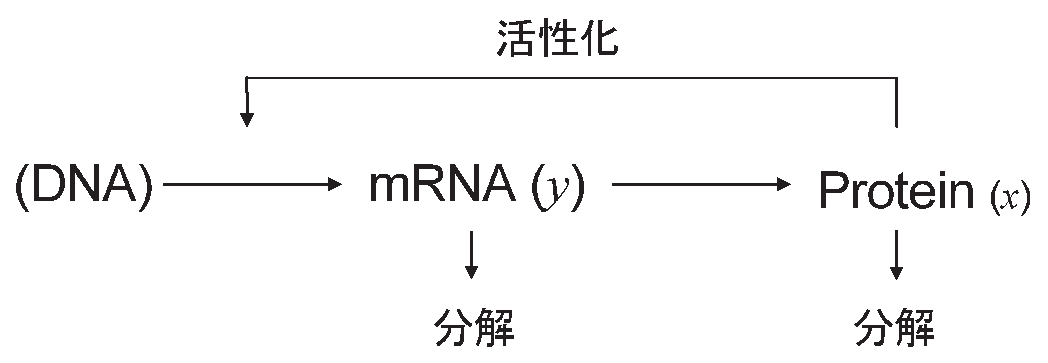
\includegraphics[height=2cm]{../Dynamical/img/griffith_model.eps}
        \caption{Griffithモデル。翻訳されたタンパク質は自身をコードする遺伝子の転写を活性化する。}
        \label{fig:04sysbio} \end{figure}

\[
\left\{
\begin{array}{lclclll}
\dot x & = & -ax + y\\
\dot y & = & \displaystyle\frac{x^2}{1+x^2} - by\\
\end{array}
\right.\]

Griffithモデルはパラメータ\(a\)、\(b\)の値によってSaddleとNodeの個数が変わるSaddle-Node分岐を示します。

\subsection{相平面とヌルクライン}
\paragraph{相平面(phase plane)}
時間とともに変化する変数を縦軸・横軸にそれぞれ取った平面のこと。例えばGriffithモデルの相平面は、mRNA(\(y\))、Protein(\(x\))をそれぞれ縦軸・横軸に取った座標空間です。

\paragraph{ヌルクライン(nullcline)} 一般に、時間変化する量についての微分方程式が0と等しくなるような点の集合をヌルクライン(nullcline)と呼びます。
相平面上に描いたヌルクラインは図\ref{fig:05sysbio}のようになります。2変数系の場合、2つのヌルクラインの交点に
おいては系が定常状態になります。非線形力学系の分野では固定点(fixed point)と呼ばれます。

\paragraph{演習1:  Griffithモデルの相平面とヌルクライン}
Griffith モデルのヌルクラインを相平面上に描きなさい。

\subsection{ベクトル場}
\paragraph{ベクトル場(vector field)}
化学反応系が相平面上の一点で表される状態にあるとき、微小時間後にその点がどの方向に動くかをベクトルで示したもの。
描き方は次の通りです。

\[
\left\{
\begin{array}{lclclll}
\dot x & = & f(x,y)\\
\dot y & = & g(x,y)\\
\end{array}
\right.\]

という2変数の系があるとき、点\((x,y)\)に大きさ\((\dot x , \dot y)\)のベクトルを描きます。
下記のような具体例を考えましょう。

\[
\left\{
\begin{array}{lclclll}
\dot x & = & -x + 2y + x^2y\\
\dot y & = & 8 -2y -x^2y\\
\end{array}
\right.\]

この系において、点\((x,y)=(1,2)\)におけるベクトルを求めてみましょう。\((x,y)=(1,2)\)を
この微分方程式に代入すると、\((\dot x, \dot y)=(5,2)\)となります。これより、\(x\)方向に5、\(y\)方向
に2の大きさを持つベクトルを点(1,2)を原点として描けばよいことになります。\\

\indent ヌルクラインの定義より、\(x\)のヌルクライン上ではベクトルは垂直(\(\dot x = 0\))になります(図\ref{fig:05sysbio})。。

\begin{figure}[ht]
        \centering 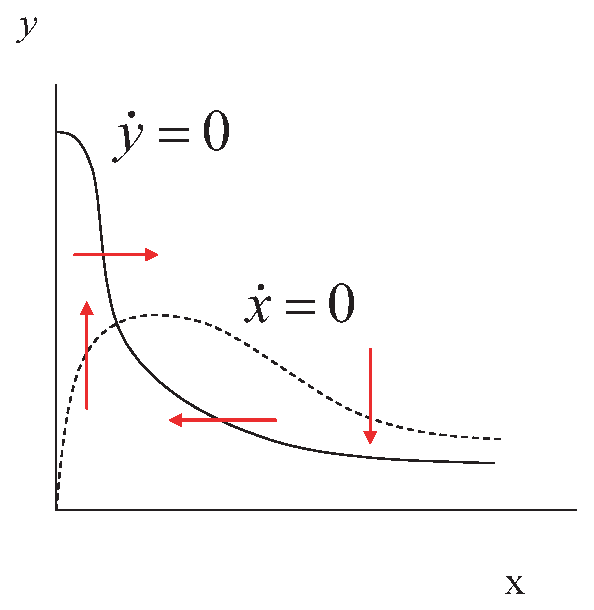
\includegraphics[height=6cm]{../Dynamical/img/vectorfield.eps}
        \caption{相平面上に描いたヌルクラインとベクトル場}
        \label{fig:05sysbio} \end{figure}


\paragraph{演習2:  Griffithモデルのベクトル場}
「演習1」の結果にベクトル場の概略を描き加えなさい。


\subsection{線形化とヤコビ行列}
\paragraph{線形化(linearization)}
非線形の微分方程式を固定点の近傍でテイラー展開し、1次の項のみ残して2次以降の項を消去すること。

\paragraph{ヤコビ行列(Jacobian matrix)}
線形化を行った結果得られた1次項からなる正方行列のこと。線形化の手順は次の通りです。
\[
\left\{
\begin{array}{lclclll}
\displaystyle\frac{d}{dt}x_1 & = & F_1(x_1, \cdots , x_n)\\
                & \vdots & \\
\displaystyle\frac{d}{dt}x_n & = & F_n(x_1, \cdots , x_n)\\
\end{array}
\right.
\]

のような連立常微分方程式を固定点\(x_{k(fp)}\)の近傍でテイラー展開すると、

\[
\begin{array}{ccl}
\displaystyle\frac{d}{dt}
\left(
\begin{array}{c}
x_{1(fp)}+\Delta x_1\\
\vdots \\
x_{n(fp)}+\Delta x_n\\
\end{array}
\right)
& = &
\left(
\begin{array}{c}
F_{1(fp)}(x_1, \cdots , x_n)\\
\vdots \\
F_{n(fp)}(x_1, \cdots , x_n)\\
\end{array}
\right)

+

\left(
\begin{array}{ccc}
\frac{\partial F_1}{\partial x_1} & \cdots & \frac{\partial F_1}{\partial x_n} \\
\vdots                            &        & \vdots\\
\frac{\partial F_n}{\partial x_1} & \cdots & \frac{\partial F_n}{\partial x_n} \\
\end{array}
\right)
\left(
\begin{array}{c}
\Delta x_1\\
\vdots \\
\Delta x_n\\
\end{array}
\right)\\

&
+
&
\displaystyle\frac{1}{2}
\left( \Delta x_1 , \cdots , \Delta x_n \right)
\left(
\begin{array}{ccc}
\frac{\partial^2 F_1}{\partial x_1^2} & \cdots & \frac{\partial^2 F_1}{\partial x_1 \partial x_n} \\
\vdots                            &    \ddots    & \vdots\\
\frac{\partial^2 F_n}{\partial x_n \partial x_1} & \cdots & \frac{\partial^2 F_n}{\partial x_n^2} \\
\end{array}
\right)
\left(
\begin{array}{c}
\Delta x_1\\
\vdots \\
\Delta x_n\\
\end{array}
\right)\\

\end{array}
\]

を得ます(3次項以降省略)。このうち、固定点の定義より\(F_k(x_{1(fp)}, \cdots , x_{n(fp)})=0\)なので0次の項は
無視できます。また、2次の項\((\Delta x_{k(fp)})^2\)は微小量の2乗ですから、固定点近傍においては2次の項を近似的に0とみなして無視することができます。
よって下記のような式が得られます。

\[
\frac{d}{dt}
\left(
\begin{array}{c}
\Delta x_1\\
\vdots \\
\Delta x_n\\
\end{array}
\right)
=
\left(
\begin{array}{ccc}
\frac{\partial F_1}{\partial x_1} & \cdots & \frac{\partial F_1}{\partial x_n} \\
\vdots                            &        & \vdots\\
\frac{\partial F_n}{\partial x_1} & \cdots & \frac{\partial F_n}{\partial x_n} \\
\end{array}
\right)
\left(
\begin{array}{c}
\Delta x_1\\
\vdots \\
\Delta x_n\\
\end{array}
\right)\\
\]

ベクトル表記にすると、

\[ \frac{d}{dt}\Delta {\bf x} = {\bf J}\Delta {\bf x}\]

右辺に残った1階偏微分からなる行列{\bf J}をヤコビ行列と呼びます。


\paragraph{演習3:  Griffithモデルの線形化とヤコビ行列}
Griffith モデルを線形化し、ヤコビ行列を求めなさい。

\subsection{ヤコビ行列の固有値と安定性}
\paragraph{行列指数関数(matrix exponential)}
線形化した連立微分方程式の解となる関数です。上で得た微分方程式

\[ \frac{d}{dt}\Delta {\bf x} = {\bf J}\Delta {\bf x}\]

の解は下記のようになります。

\[\Delta {\bf x}=\exp({\bf J}t)\Delta {\bf x}_0\]

ただし、

\[\exp({\bf J}t) = {\bf I} + \frac{{\bf J}t}{1!} + \frac{{\bf J}^2 t^2}{2!} + \frac{{\bf J}^3 t^3}{3!} + \cdots\]

であり、\(\Delta {\bf x}_0\)は系に与えられた摂動の大きさ(固定点からのずれの初期値)です。

\paragraph{固有値(eigenvalue)}
行列指数関数は後々扱いが面倒なので、ヤコビ行列{\bf J}の固有値\(\lambda\)・固有ベクトル{\bf v}を用いて普通の指数関数に書き直しておきます。

\begin{eqnarray*}
\exp({\bf J}t){\bf v} & = & \left({\bf I} + \frac{{\bf J}t}{1!} + \frac{{\bf J}^2 t^2}{2!} + \frac{{\bf J}^3 t^3}{3!} + \cdots \right){\bf v}\\
                      & = & \left(1 + \frac{\lambda t}{1!} + \frac{\lambda^2 t^2}{2!} + \frac{\lambda^3 t^3}{3!} + \cdots \right){\bf v}\\
                      & = & \exp(\lambda t) {\bf v}\\
\end{eqnarray*}

また、初期摂動\(\Delta {\bf x}_0\)も固有ベクトルの線形結合として下のように表せます。

\[\Delta {\bf x}_0 = c_1 {\bf v}_1 + \cdots c_n {\bf v}_n \]

幾何学的な描像を図\ref{fig:06sysbio}に示しました。

\begin{figure}[ht]
        \centering 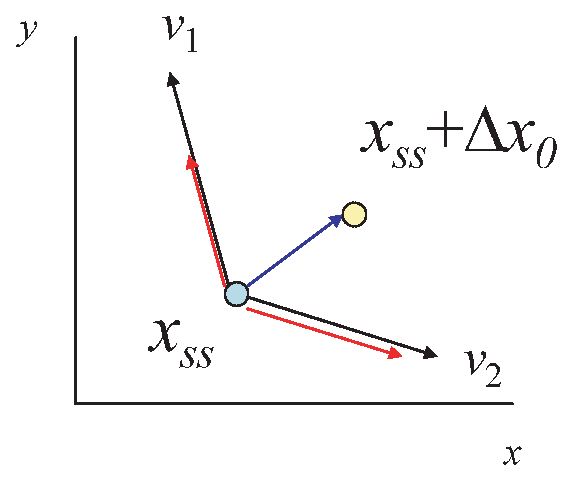
\includegraphics[height=6cm]{../Dynamical/img/decomposition.eps}
        \caption{摂動(定常状態\(x_{ss}\)からのずれ)は固有ベクトルの線形結合として表せる。}
        \label{fig:06sysbio} \end{figure}


よって、固定点からのずれ\(\Delta {\bf x}\)は、

\begin{eqnarray*}
\Delta {\bf x}(t) & = & \exp({\bf J}t)\Delta {\bf x}_0\\
                 & = & \exp({\bf J}t)(c_1 {\bf v}_1 + \cdots c_n {\bf v}_n) \\
                 & = & c_1 \exp(\lambda_1 t){\bf v}_1 + \cdots c_n \exp(\lambda_n t){\bf v}_n \\
\end{eqnarray*}

となり、固有値が正の時には\(\Delta {\bf x}\)が発散し、負の時には収束する(すなわち固定点に戻る)ことがわかります(図\ref{fig:07sysbio})。

\begin{figure}[ht]
        \centering 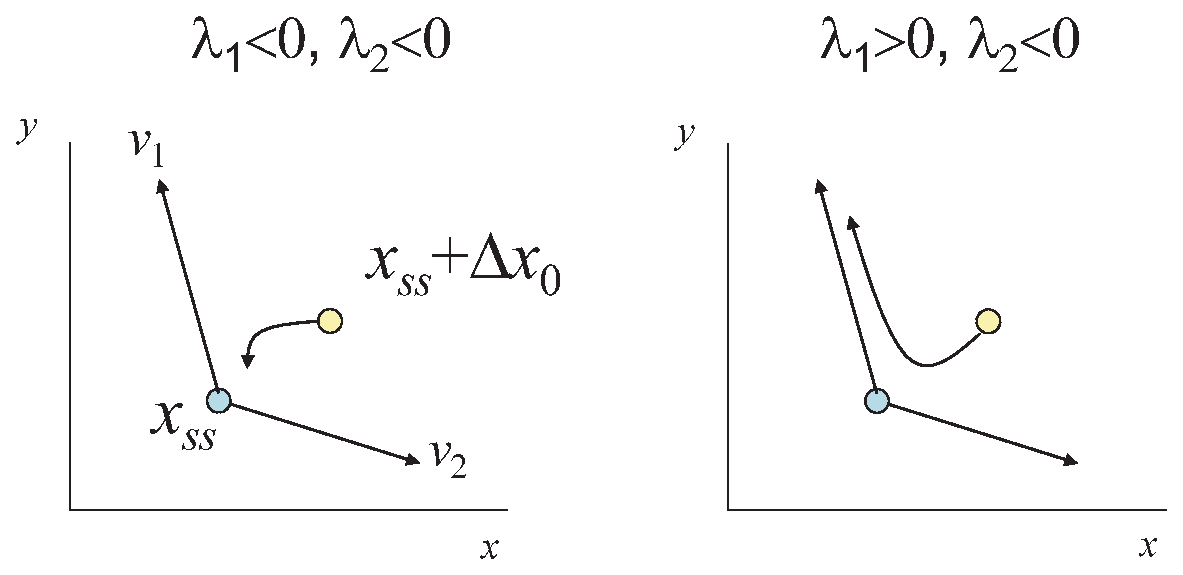
\includegraphics[height=5cm]{../Dynamical/img/eigenvector.eps}
        \caption{(左)固有値がすべて負なら解軌跡は固定点に収束する。(右)正の固有値を含む固定点では解軌跡が発散する。}
        \label{fig:07sysbio} \end{figure}


\paragraph{固定点の分類} ヤコビ行列の固有値の正負・虚実の組み合わせにより、固定点は下表のように分類されます。注目している化学反応系の固定点がどのタイプにあたるのかを調べることで、化学反応系の動態を定性的に把握できます(図\ref{fig:08asysbio}、 \ref{fig:08bsysbio})。\\

\begin{center}
表: 固有値による固定点の分類\\
\begin{tabular}{clll}
\hline
固有値の虚実 & 固有値の符号       & 固定点の名称 & 時系列の特徴 \\
\hline
実数  & すべて正         & Unstable node  & 不安定な定常状態\\
   & すべて負         & Stable node    & 安定した定常状態\\
      & 正負混在         & Saddle         & 不安定な定常状態\\
\hline
複素数 & 実部がすべて負  & Stable spiral  & 減衰振動(安定解)\\
    & 正の実部を持つ  & Unstable spiral & 発散振動(不安定解)\\
       & 純虚数          & Center          & 調和振動\\
\hline
\end{tabular}
\end{center}

\begin{figure}[ht]
        \centering 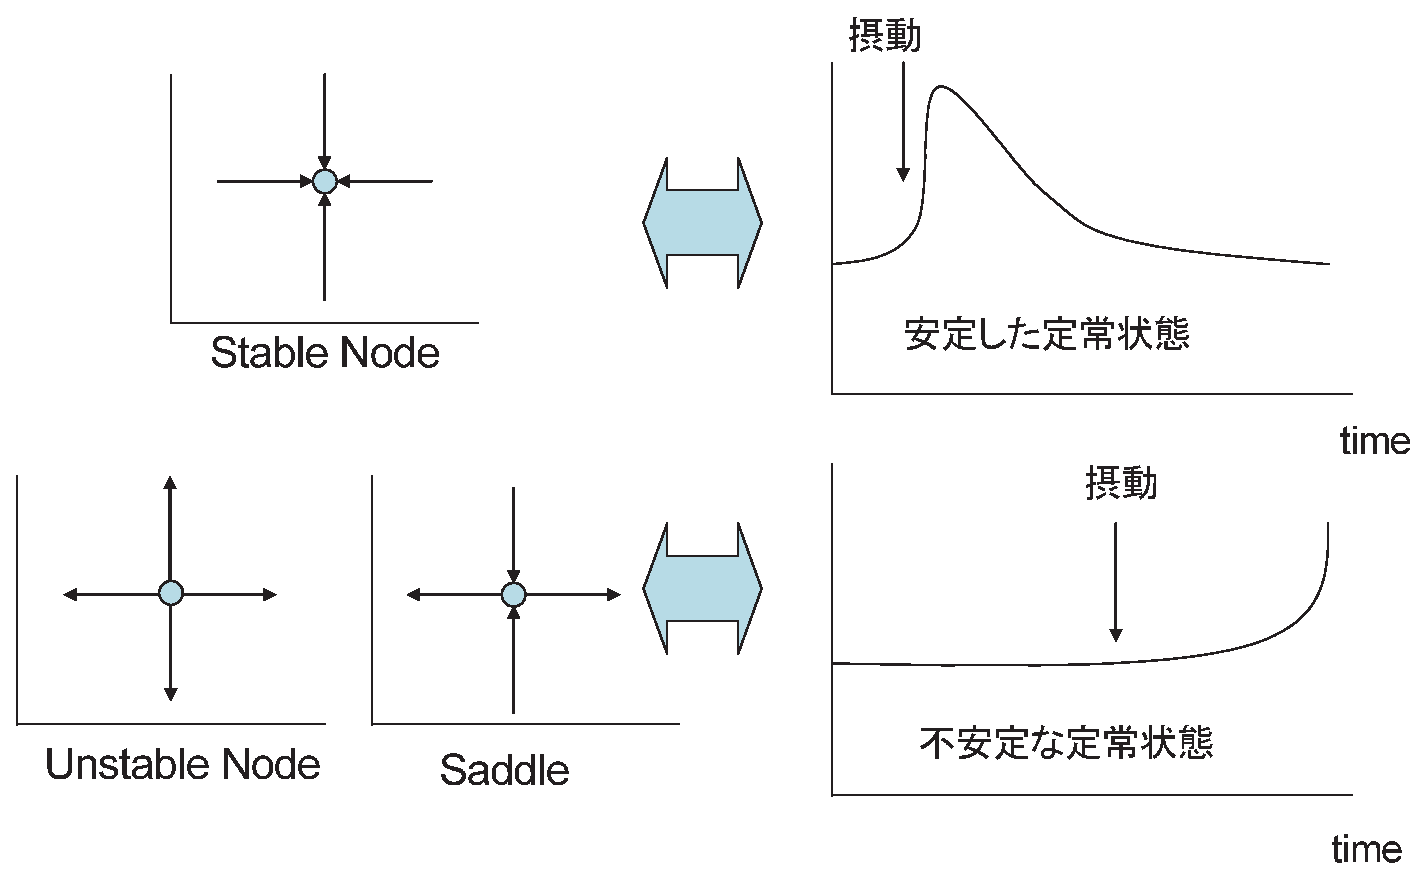
\includegraphics[height=6cm]{../Dynamical/img/node_stability.eps}
                \caption{実数固有値のみの場合の固定点の分類。(左)それぞれの固定点近傍におけるベクトル場の特徴。正の固有値を1つでも含むと不安定な定常状態となる。(右)時系列の特徴。}
        \label{fig:08asysbio} \end{figure}
        
\begin{figure}[ht]
        \centering 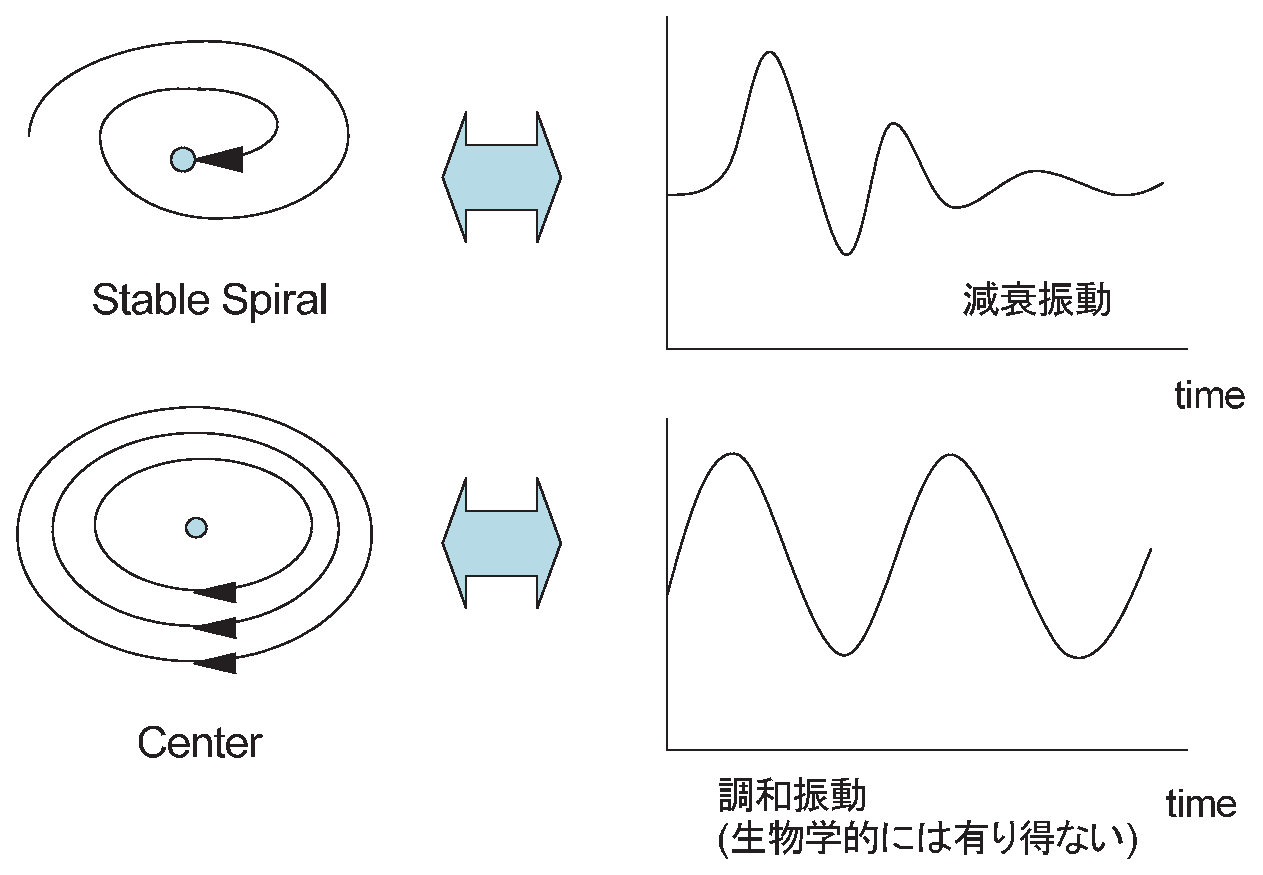
\includegraphics[height=6cm]{../Dynamical/img/spiral_stability.eps}
        \caption{複素固有値を含む場合の固定点の分類。(左)それぞれの固定点近傍におけるベクトル場の特徴。実部の符号によって安定性を判別する。(右)時系列の特徴。}
        \label{fig:08bsysbio} \end{figure}


\paragraph{固有値の正負・虚実の判別法}
ヤコビ行列が2行2列の場合、下記のようにすると固有方程式を解かずに固有値の符号を知ることができます。ヤコビ行列を

\[{\bf J} =
\left(
\begin{array}{rr}
a& b\\
c& d\\
\end{array}
\right)
\]

とおくと、固有方程式は\(\lambda^2-(a+d)\lambda+(ad-bc)=0\)となります。この固有方程式の2つの解を\(\lambda_1\) 、\(\lambda_2\)とすると、2次方程式の解と係数の関係から、

\[
\begin{array}{lclclcl}
\tau & = & \lambda_1 + \lambda_2 & = & a + d & = & {\rm tr}({\bf J})\\
\Delta & = &\lambda_1 \lambda_2 & = & ad - bc & = & \det({\bf J})\\
\end{array}
\]

と書くことができます。\(\Delta\)の正負から、2つ固有値(の実部)が同符号であるか判定でき、その符号が正負どちらなのかは\(\tau\)の正負に対応します。また、\(\tau^2 -4\Delta\)の正負からは固有値が実数・複素数のどちらになるかを判定できます。


\paragraph{演習4:  Griffithモデルにおける固定点の分類}
ヤコビ行列の固有値の符号を調べ、Griffith モデルに現れる固定点を分類しなさい。

\subsection{分岐}
\paragraph{分岐(bifurcation)} パラメータの変化により、固定点の数や種類が変わること。Griffith モデルはパラメータの値によって、固定点の数、安定性が変わるSaddle-Node分岐を示します。

\paragraph{演習5:  Griffithモデルにおける分岐}
\(ab < \displaystyle\frac{1}{2}\)、\(ab=\displaystyle\frac{1}{2}\) 、\(ab > \displaystyle\frac{1}{2}\) の3つの場合についてベクトル場を描きなさい。固定点の個数、性質はどのように3つの場合でどのように異なっているか。


\section{Hopf(ホップ)分岐}
%\documentclass[a4paper,11pt]{jsarticle}
%\usepackage{graphicx}
%\usepackage{ascmac}
%\usepackage{url}

\def\演習問題#1{{\flushleft\underline{\bf 演習問題~#1}}}

%\begin{document}
\subsection{Sel'kov モデル: 振動現象}
\indent 比較的早くから見つかっていた生物リズムとして、出芽酵母解糖系に
おける物質濃度の振動があります。Sel'kovは1968年に図\ref{fig:09sysbio}
に示すモデルを提案し、解糖系の流束に影響力を持つ酵素であ
るphosphofructokinase(PFK)周辺のフィードバック・ループが振動子の核心で
あると主張しました。以降、このSel'kovモデルは生物リズムを説明する最もシ
ンプルな模型として多くの論文や教科書で取り上げられています。ここで
はSel'kovモデルを通じて振動現象を説明する数理を学びます。

\begin{figure}[ht]
        \centering 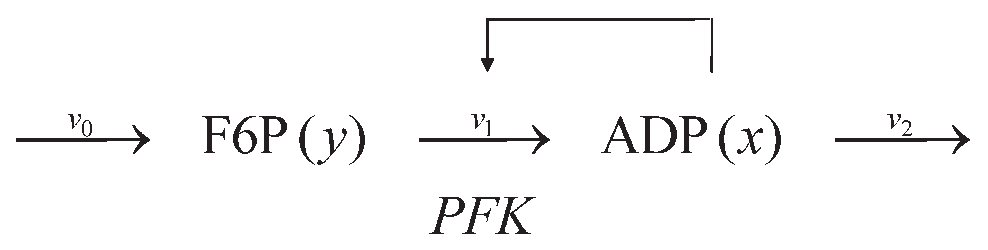
\includegraphics[height=1.5cm]{../Dynamical/img/selkov_model.eps}
        \caption{Sel'kovモデル。ADPがPFKを活性化することによる正のフィードバック・ループを持つ。}
        \label{fig:09sysbio} \end{figure}

連立微分方程式で図\ref{fig:09sysbio} を表現したものを次に示します。

\[
\left\{
\begin{array}{lclclll}
\dot x & = & -x+ay+x^2 y\\
\dot y & = & b-ay-x^2y\\
\end{array}
\right.\]

ただし、\(x\)はADP、\(y\)はF6Pの存在量です。

\paragraph{リミットサイクル(limit cycle)} 相平面中にできる閉曲線。非線形振動の軌跡に相当します。
Center周囲には同心円状に閉軌道が存在する(図\ref{fig:08bsysbio})のに対し、リミットサイクルの周辺には
閉軌道は存在しません(図\ref{fig:09sysbio}右)。固有値を\(\lambda = a+bi\)とおいたとき、振動の周期はおおよそ\(\displaystyle\frac{2\pi}{b}\)となります。実習課題(3)で描いた概日時計モデルの解軌跡もリミットサイクルです。

\paragraph{Hopf 分岐 (Hopf bifurcation)}
振動現象ときわめて密接な関係にある分岐です。共役な複素固有値対が複素平面の虚軸を左から右に横切るとき(すなわち実部が負から正になるとき)、Stable spiralがUnstable spiralに変化することを指します。{\bf Hopf分岐が存在する場合、Unstable node の周囲にはリミットサイクルが存在することが保証されています。}よってHopf分岐により、系が定常状態から振動状態へとその挙動を変えます。
細胞内における分子濃度の振動現象のほとんどは Hopf 分岐で説明できます。

\begin{figure}[ht]
        \centering 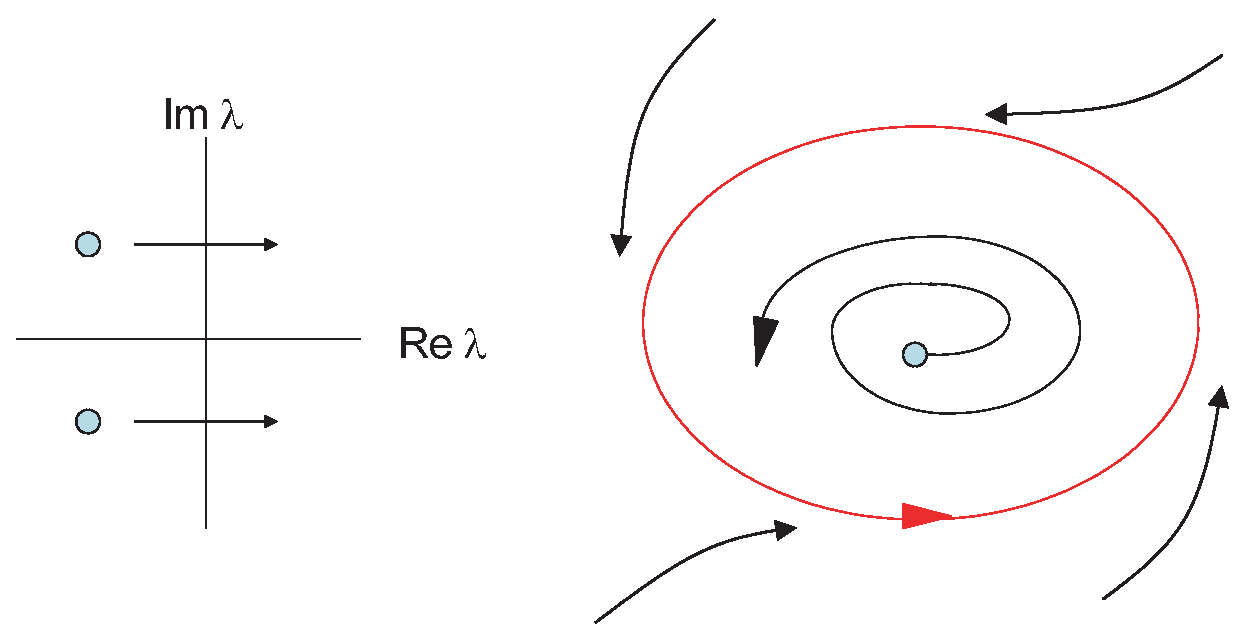
\includegraphics[height=6cm]{../Dynamical/img/hopf_limitcycle.eps}
        \caption{(左)共役な複素固有値対が虚軸を左から右に横切るとき、Stable spiralがUnstable spiralに変化する。(右)これに伴い、Unstable spiral を取り巻くようにリミットサイクル(赤で描いた閉軌道)が生じる。}
        \label{fig:10sysbio} \end{figure}


\subsection{演習: Sel'kov モデルの解析}
\begin{enumerate}
\item Sel'kov モデルのヌルクラインを相平面上に描きなさい。
\item 「1」の結果にベクトル場の概略を描き加え、固定点がSpiralになると予想できることを確かめなさい。
\item Sel'kov モデルを線形化し、ヤコビ行列を求めなさい。
\item 2つの固有値の実部が同符号であることを確認しなさい(ヒント: \(\Delta\)の正負を調べる)。
\item Sel'kov モデルの固定点が Stable Spiral から Unstable Spiral へと変化するときに パラメータ\(a\)、\(b\)の間に成り立つ関係式を求めなさい(ヒント: \(\tau\)=0となる条件を調べる。理由はなぜか?)。
\item 「5」で求めた式に相当する曲線の概形を描きなさい。\(a\)、\(b\)をそれぞれ横軸、縦軸とすること。曲線を境に、どちら側がStableもしくはUnstableなのかも記入しなさい。
\end{enumerate}



\section{Pitchfork(熊手型)分岐}
\subsection{Toggle switch}
ボストン大学Collins lab.のGardnerらは、互いに抑制し合う遺伝子から成る人工遺伝子回路(図\ref{fig:11sysbio})を構築し、大腸菌細胞内で双安定スイッチ(toggle switch)として動作させることに成功しました。同じように双安定性を示す Griffith モデルが Saddle-Node 分岐を内包していたのとは異なり、Toggle switch は1個もしくは3個の固定点を持つ Pitchfork 分岐を起こします。

\begin{figure}[ht]
        \centering \includegraphics[height=3cm]{../Dynamical/img/toggleswitch.epsi}
        \caption{GardnerらのToggle switch型遺伝子回路。2つのリプレッサーが、互いを抑制し合う。}
        \label{fig:11sysbio} \end{figure}

連立微分方程式で図\ref{fig:11sysbio} を表現したものを次に示します。

\[
\left\{
\begin{array}{lcl}
\dot x & = & \displaystyle\frac{a}{1+y^2} - x\\
\dot y & = & \displaystyle\frac{a}{1+x^2} - y\\
\end{array}
\right.
\]

式の形を見ると、\(x\)と\(y\)を置換しても同じ式になることがわかります。Pitchfork分岐はこのように対称性をもつ系に生じる分岐です(図\ref{fig:12sysbio})。

\begin{figure}[ht]
        \centering \includegraphics[height=3cm]{../Dynamical/img/pitchfork.epsi}
        \caption{Pitchfork分岐の際の固定点のy座標の変化。分岐点を境に、固定点が1個から3個に増える。全体の形状が熊手(pitchfork)に似ているのが命名の由来。}
        \label{fig:12sysbio} \end{figure}


\subsection{演習: Toggle switch モデルの解析}
\begin{enumerate}
\item Toggle switch モデルのヌルクラインを相平面上に描きなさい。固定点の数は\(a\)の値によって1個または3個になりますが、どちらの場合でも構いません。
\item 「1」の結果にベクトル場の概略を描き加え、固定点が1個の場合はStable Nodeに、3個の場合はStable Node 2個とUnstable Node 1個になると予想できることを確かめなさい。
\item \(y\)についてのヌルクラインの式を\(x\)についてのヌルクラインの式に代入し、固定点の\(x\)座標が\(x^5-ax^4+2x^3-2ax^2+(1+a^2)x-a=0\)を満たすことを示しなさい。
\item 「3」で示した固定点\(x\)座標に関する条件式\(x^5-ax^4+2x^3-2ax^2+(1+a^2)x-a=0\)が\((x^3+x-a)(x^2-ax+1)=0\)と因数分解できることを確認しなさい。
\item 一般に、\(x^3+ax+b=0\) の形をした3次方程式の解の性質は、判別式\(D=-4a^3-27b^2\)で予測することができる。\(D>0\)ならば3つの実数解、\(D=0\)ならば重解、\(D<0\)ならば1つの実数解と2つの虚数解を持つ。因数分解によって生じた\(x^3+x-a\)について、\(x^3+x-a=0\)について1つの実数解と2つの虚数解があることを確認しなさい。
\item 2次方程式の部分 \(x^2-ax+1\) の解の判別式を求め、\(a=2\)を境に固定点が1個から3個に変化することを確認しなさい。
\item \(a>2\)のとき、2次方程式の部分 \(x^2-ax+1\) から求まる固定点について、ヤコビ行列の2つの固有値がともに負となることを確認しなさい(ヒント: \(\Delta\)の正負を調べる)
\end{enumerate}

\section{Further reading}
\noindent Strogatz, S.H, “Nonlinear dynamics and chaos”, Perseus Books Publishing, 1994. (ISBN 0-7382-0453-6)\\
(バイオロジストにとって最良の非線形力学系教科書。Borisuk and Tyson (1998)の背景知識学習にも最適。)\\

\noindent Fall, C.P., Marland, E.S., Wagner, J.M. and Tyson, J.J. “Computational cell biology”, Springer, 2002. (ISBN 0-387-95369-8)\\
(Bendixsonの基準など、振動を起こす系の必要十分条件に関する記述がわかりやすい。)\\

\noindent Borisuk, M.T. and Tyson, J.J., “Bifurcation analysis of a model of mitotic control in frog eggs”, J. Theor. Biol. 195:69-85, 1998.\\
(アフリカツメガエルの卵における細胞周期調節に関するモデル解析。ありとあらゆる分岐が登場するので、ケーススタディに最適。)\\

\noindent Griffith, J.S. Mathematics of cellular control processes. II. Positive feedback to one gene. J. Theor. Biol. 20, 209-16, 1668.\\
(Griffithモデルの初出論文。)\\

\noindent Sel'kov, E.E., Self-oscillations in glycolysis. 1. A simple kinetic model. Eur J Biochem. 4(1):79-86, 1968.\\
(Sel'kov モデルの初出論文。)\\

\noindent Gardner, T.S., Cantor, C.R. and Collins, J.J., Construction of a genetic toggle switch in Escherichia coli., Nature 403(6767):339-42, 2000.\\
(Toggle switch の初出論文。)\\

%\section{Poincar\'{e}-Bendixsonの定理}
%\section{Bendixsonの基準}

%\end{document}

%\chapter{酵素反応速度論}
\section{目標}
Joshi and Palsson, Huang and Ferrelを読める
\section{Mass action}
\section{Michaelis-Menten式}
\section{King-Altman法}
\section{MWC, KNF}
\section{Hill式}
\section{迅速平衡、Time scale decomposition}
\section{Further reading}
酵素キネティクス
Heinrich and Schuster






%\chapter{反応速度{\it k}の物理学}
\section{目標}
「活性化エネルギー」を読める
1分子同士の衝突頻度=衝突「確率」、といってよいか?

\section{自由エネルギーとは何か}
\section{熱力学関数}
\subsection{示量・示強}
\subsection{記憶図とLegendre変換}
\section{Boltzmann分布}
\section{Maxwell分布}
\section{前頻度因子の導出}
\subsection{古典衝突理論}
\subsubsection{剛体球衝突モデル}
\section{親和力と反応速度}

\begin{eqnarray*}
Z_t & = & \sigma (v_r) v_r dc_A dc_B\\
\end{eqnarray*}

\(v_r\)分子AとBの相対速度、\(\sigma(v_r)\)分子AとBの衝突断面積。分子Aの半径を\(r_A\)、分子Bの半径を\(r_B\)とすると\(\sigma = 4 \pi (r_A + r_B)^2\)。

ここでMaxwell-Boltzmannの速度分布を用いて、

\subsubsection{反応性衝突モデル}
ただぶつかっただけでは反応しない。2分子反応\(A+B \longrightarrow C+D\)の速度\(v\)は\(v=k[A][B]\)と表される。反応速度は単位体積あたりの反応性衝突に等しい。

\begin{eqnarray*}
v & = & k[A][B]\\
  & = & Z_r\\
  & = & \left\{ \sigma_{AB} \left(\frac{8k_B T}{\pi \mu}\right)^{\frac{1}{2}}{\rm exp}\left(-\frac{\varepsilon_t^{0}}{k_B T}\right) \right\} [A][B]\\
\end{eqnarray*}



\subsection{絶対反応論}

\section{演習: 遷移状態理論と速度定数}
分子動力学(MD)シミュレーションにより、ある反応が起こる前と後での内部エネルギー変化は\(\Delta U = 1.23\)J/molであることが示された。系の温度を310K、エンタルピー変化\(\Delta H \simeq \Delta U\)として次の問いに答えなさい。

\begin{enumerate}
\item エントロピー変化\(\Delta S\)はどのくらいか。\({\displaystyle \Delta S = \frac{\Delta U}{T}}\)である。
\item Eylingの遷移状態理論によれば、速度定数\(k\)は以下の式で表される。MDから求まった\(\Delta H\)、\(\Delta S\)が使えるよう、熱力学の第1法則\(\Delta G = \Delta H - T \Delta S\)を用いて書き直しなさい。
\[k = \frac{k_B T}{h}\kappa e^{-\frac{\Delta G^0}{RT}}\]
\item MDから求まった\(\Delta H\)、\(\Delta S\)を代入して、速度定数\(k\)を求めなさい。
\end{enumerate}


\section{Further reading} 
活性化エネルギー
反応の自由エネルギー変化についてはアイゼンバーグ&クロサーズ
熱力学 キャレン(記憶図)、田崎(ルジャンドル変換)、清水、原島と小出(束縛エネルギー)
統計力学 高校数学で分かるボルツマンの原理、名古屋大の上羽先生のPDF

量子化学計算
吉澤先生の論文
平尾 量子化学計算ビギナーズマニュアル

%\chapter{常微分方程式の数値積分法}
%\chapter{常微分方程式の数値積分法 I: 1段階法と多段階法、陽的解法と陰的解法}
本章の目標はMATLABに装備されている数値積分法の仕組みを理解することにある。Runge-Kutta法の次数、Butcher表の見かた、陽的、陰的、埋め込み型、可変ステップ、硬い方程式といった概念を理解し、適切な数値積分アルゴリズムを選択する判断力を身に付けることを目指す。

\section{Taylor 展開の式を使わないのはなぜか?}
数値積分はTaylor展開と比べてどこがいいのか?

\[y(x_0 + h) = y(x_0) + h \cdot y^{\prime}(x_0) + \frac{h^2}{2!} y^{\prime  \prime}(x_0) + \cdots\]

Taylor展開では、高階微分の項が複雑になる。数値積分公式は、微分項の計算なしに積分ができるすぐれものの近似式である。

\section{分類}
\begin{tabular}{l||c|c}
      & 1段階法               & 多段階法 \\
\hline
陽公式 & Euler, Runge-Kutta   & Adams \\
\hline
陰公式 & Implicit Euler, Implicit Runge-Kutta   & Gear \\
\hline
\end{tabular}
\\

陽公式 左辺 \(y_{n+1}\) 、右辺 \(y_{n}\) など (n+1未満) 陰公式 左
辺 \(y_{n+1}\) 右辺も \(y_{n+1}\)。まず陽公式で\(y_{n+1}\)を予測し、そ
れを陰公式に代入して修正する、といった使い方をする。

%1段階法:  y_n+1 = a * y_n 
%多段解法: y_n+1 = a* y_n + b * y_n-1 + ... + p * y_n-m

\section{紙と鉛筆の限界を知る}
線形なら対角化すれば解析的に解ける。

\[
\left\{
\begin{array}{lll}
\frac{d}{dt}[A] & = & - 2k [A] \\
\frac{d}{dt}[B] & = & 2k [A] - k[B]\\
\frac{d}{dt}[C] & = & k [B] \\
\end{array}
\right.
\]



\[
\frac{d}{dt}
\left(
\begin{array}{r}
A\\
B\\
C\\
\end{array}
\right)
=
\left(
\begin{array}{rrr}
-2 & 0 & 0\\
2 & -1 & 0\\
0 & 1 & 0\\
\end{array}
\right)
\left(
\begin{array}{r}
A\\
B\\
C\\
\end{array}
\right)
\begin{array}{r}
\ \\
\ \\
, \\
\end{array}
 \left(
\begin{array}{r}
A_0 \\ 
B_0 \\
C_0 \\
\end{array}
\right)
=
\left(
\begin{array}{r}
1\  {\rm mM} \\
0\  {\rm mM} \\
0\  {\rm mM} \\
\end{array}
\right)
\]


\[\frac{d}{dt}{\mathbf x} = {\mathbf A}{\mathbf x}\]


\begin{eqnarray*}
{\mathbf A}{\mathbf P} & = & {\mathbf P}{\mathbf \Lambda}\\
{\mathbf P}^{-1}{\mathbf A}{\mathbf P} & = & {\mathbf \Lambda}\\
{\mathbf P}^{-1}{\mathbf A} & = & {\mathbf \Lambda}{\mathbf P}^{-1}\\
\end{eqnarray*}

\begin{eqnarray*}
{\mathbf P}^{-1}\frac{d}{dt}{\mathbf x} & = & {\mathbf P}^{-1}{\mathbf A}{\mathbf x} \\
\frac{d}{dt}({\mathbf P}^{-1}{\mathbf x}) & = & {\mathbf \Lambda}({\mathbf P}^{-1}{\mathbf x}) \\
\end{eqnarray*}

\[
\frac{d}{dt}{\mathbf P}^{-1}{\mathbf x} 
= 
\left(
\begin{array}{rrr}
0 & 0 & 0 \\
0 & -1 & 0 \\
0 & 0 & -2 \\
\end{array}
\right)
{\mathbf P}^{-1}{\mathbf x}
\]

\begin{eqnarray*}
{\mathbf P}^{-1}{\mathbf x} 
& = &
\left(
\begin{array}{c}
C_1 \\
C_2 \exp(-t)\\
C_3 \exp(-2t)\\
\end{array}
\right)\\
 & = &
\left(
\begin{array}{rrr}
1 & 1 & 1 \\
2 & 1 & 0 \\
1 & 0 & 0 \\
\end{array}
\right)
\left(
\begin{array}{rrr}
A\\ 
B\\
C\\
\end{array}
\right)
\end{eqnarray*}

よって

\begin{eqnarray*}
A + B + C & = & C_1 \\
2A + B    & = & C_2 \exp(-t) \\
A         & = & C_3 \exp(-2t)\\ 
\end{eqnarray*}

\[
\left(
\begin{array}{r}
A_0 \\ 
B_0 \\
C_0 \\
\end{array}
\right)
=
\left(
\begin{array}{r}
1\  {\rm mM} \\
0\  {\rm mM} \\
0\  {\rm mM} \\
\end{array}
\right)
\]
より \(C_3 = 1\)、\(C_2 = 2\)、\(C_1 = 1\)とわかる。

\begin{eqnarray*}
A + B + C & = & 1 \\
2A + B    & = & 2 \exp(-t) \\
A         & = & \exp(-2t)\\ 
\end{eqnarray*}

この連立方程式を解いて、

\[
\left(
\begin{array}{r}
A \\ 
B \\
C \\
\end{array}
\right)
=
\left(
\begin{array}{c}
\exp(-2t) \\
2\exp(-t) - 2\exp(-2t) \\
1 - 2\exp(-t) + \exp(-2t) \\
\end{array}
\right) {\rm mM}
\]

\section{1段階法}
\subsection{陽的な1段階法: Euler法}
最も単純な数値積分アルゴリズムはEuler法です。定義としては、Taylor展開の式

\[y(x_0 + h) = y(x_0) + h \cdot y^{\prime}(x_0) + \frac{h^2}{2!} y^{\prime  \prime}(x_0) + \cdots\]

から2次以降の項を取り除いた次の式がEuler法です。

\[y(x_0 + h) = y(x_0) + h \cdot y^{\prime}(x_0) \]

Euler法の近似精度は、Taylor展開式の1次までの精度と同等です。

\indent これだと一般的すぎるので、生物の場合にあてはめて考えてみましょ
う。時刻tにおける物質Sの濃度を\(S(t)\)とし、そこから微小時間\(\Delta
t\)だけ進んだ時刻\(t+\Delta t\)における物質Sの濃度を\(S(t+\Delta t)\)で
表します。これを上のEuler法の定義に当てはめると、

\[S(t+\Delta t) = S(t) + \Delta t S^{\prime}(t)\]

となります。 \(S^{\prime}(t)\)というのはSの時間微分\(\displaystyle\frac{dS}{dt}\)のことですので、

\[S(t+\Delta t) = S(t) + \Delta t \frac{dS}{dt}\]

という式が得られます。\(\displaystyle\frac{dS}{dt}\)は反応速度式で表されます。ここではテストケースとして \(\displaystyle\frac{dS}{dt} = -k \cdot S\) としてみましょう。

\[S(t+\Delta t) = S(t) - \Delta t \cdot k \cdot S\]

これを増分の形にすると、

\begin{eqnarray*}
\Delta S(t) & = & S(t+\Delta t) - S(t)\\
            & = & - \Delta t \cdot k \cdot S\\
\end{eqnarray*}

よってEuler法を用いる場合、微小時間\(\Delta t\)の間にSがどの程度増減す
るかは\(- \Delta t \cdot k \cdot S\)で計算できることがわかりました。\\

\subsection{演習}
\begin{enumerate}
\item グルコース濃度の変動に関する常微分方程式\(\frac{d{\rm [Glucose]}}{dt}=-k{\rm [Glucose]}\)をオイラー法で解きなさい。積分ステップ幅\(\Delta t=1.0 {\rm sec}\)とし、\(t=0 \sim 5.0\) secの範囲について解くこと。反応定数\(k=0.2 {\rm sec}^{-1}\)、\(t=0\) sec のとき[Glucose]=1.0mMとする。
\item (1)の常微分方程式の解析解を求め、\(t = 5.0\) sec 時点までの数値解との時系列平均誤差\(\displaystyle\varepsilon=\frac{1}{n}\sum_{i=1}^n\frac{|X^{\rm analytical}_i - X^{\rm numerical}_i|}{ X^{\rm analytical}_i}\)を計算しなさい。
\item 積分ステップ幅\(\Delta t\)を1.0 secより大きくした場合と小さくした場合では、解析解との時系列平均誤差がどのように変化するか仮説を立てなさい。理由も述べること。
\item 仮説を検証しなさい。
\end{enumerate}

\subsection{陰的な1段階法: 陰的Euler法}

\subsection{ステップ刻み幅を決めるには「絶対安定」 の概念が必要}



\section{多段階法}
多段階法とは以下のような一般式で書ける数値積分法のことである。

\[\alpha_{0} y_{n} + \alpha_{1} y_{n-1} + \cdots + \alpha_{k} y_{n-k} = h(\beta_{0}f_{n} + \beta_{1}f_{n-1} + \cdots  + \beta_{m}f_{n-m})\]

\(y_n\)は\(t_n\)時点における\(y\)の値を意味する。また、\(y_{n-k}=y(t_n-kh)\)、\(f=y^{\prime}\)である。

\subsection{利点}
Eulerと比べてどこがいいのか?→高次の項を入れて局所離散誤差を小さくできる。RKと異なり、導関数はステップあたり1回計算すれば済む。


\subsection{陽的な多段階法: Adams-Bashforth法}
陽的な多段階法の代表例である。あまり使ったことはないが、Gear法を理解する目的で足がかりとなるので紹介する。

Adams法は

\[ y_n = \alpha_1 y_{n-1} + h( \beta_1 f_{n-1} + \beta_2 f_{n-2})\]

という形の多段階法である。係数\(\alpha, \beta\)をTaylor展開から定める。
まず上の式を書き換える。

\[ y(t_n) = \alpha_1 y(t_{n-1}) + h( \beta_1 f( t_{n-1} , y(t_{n-1}) ) + \beta_2 f( t_{n-2} , y(t_{n-2}) ))\]

\(t_{n-1} = t - h\)より、Taylor展開する。

\begin{eqnarray*}
y(t_n) & \simeq & \alpha_1 \left\{y(t_{n}) - h \frac{d}{dt} y(t_n) + \frac{h^2}{2} \frac{d^2}{dt^2} y(t_{n}) \right\} \\
 & + & h \beta_1 \left\{ f(t_n) - h \frac{d}{dt} f(t_n) + \frac{h^2}{2} \frac{d^2}{dt^2} f(t_{n}) \right\}\\
 & + & h \beta_2 \left\{ f(t_n) - 2h \frac{d}{dt} f(t_n) + \frac{4h^2}{2} \frac{d^2}{dt^2} f(t_{n}) \right\}\\
\end{eqnarray*}

hの次数が同じ項ごとに整理する。

\[
\begin{array}{lccll}
h^0 & : & y(t_n) & = & \alpha_1 y(t_n)\\
h^1 & : & 0 & = & - \alpha_1 h y^{\prime}(t_n) + h \beta_1 y^{\prime}(t_n) + h \beta_2 y^{\prime}(t_n)\\
h^2 & : & 0 & = & \alpha_1 \frac{h^2}{2} y^{\prime\prime}(t_n) - h^2 \beta_1 y^{\prime\prime}(t_n) -2 h^2 \beta_2 y^{\prime\prime}(t_n)\\
\end{array}
\]

これで、\(\alpha, \beta\)に関する連立方程式を立てることができる。

\[
\left\{
\begin{array}{lcl}
1 & = & \alpha_1 \\
0 & = & - \alpha_1 + \beta_1 + \beta_2 \\
0 & = & \frac{1}{2} \alpha_1 - \beta_1 -2 \beta_2 \\
\end{array}
\right.
\]

これを解くと、2次のAdams-Bashforth法の係数は\(\alpha_1 = 1, \beta_1 = \frac{3}{2}, \beta_2 = \frac{1}{2}\)と求まる。よってAdams-Bashforth法は

\[ y_n = y_{n-1} + h \left( \frac{3}{2} f_{n-1} + \frac{1}{2} f_{n-2}\right)\]

と書ける。
化学反応系 \(\displaystyle\frac{dS}{dt} = -k \cdot S\) にあてはめると、

\[\Delta S = \Delta t \left( - \frac{3}{2} k \cdot S_{t=t-\Delta t} - \frac{1}{2} k \cdot S_{t=t-2\Delta t}\right)\]

となる。


\subsection{陰的な多段階法: Adams-Moulton法}

\subsection{予測子修正子法}
予測子修正子(predictor-corrector)法とは、陽公式と陰公式を組み合わせて両者のいいとこどりを図る方法のことである。Adams-Bashforth法とAdams-Moulton法を組み合わせる例が有名である。MATLABのode113がこれにあたる。

\begin{tabular}{c||l|l}
      & 長所 & 短所 \\
\hline
陽公式 & 過去の値を使って、次のステップの値が出せる & 安定性で陰公式に劣る\\
陰公式 & 安定性が優れている & 現時点の値がないと計算できない \\
\end{tabular}

陽公式で予測値を計算し(予測子)、予測値をもとに現時点の値を陰公式で計算(修正子)

Backward Differential Formula(ode15s)

\section{安定性}
\subsection{絶対安定}
\subsubsection{線形テスト問題}

\subsubsection{多段階法}
安定性多項式の根がすべて1未満。
\paragraph{安定性多項式}
\subsubsection{Runge-Kutta法}


%\chapter{常微分方程式の数値積分法 II: Runge-Kutta法}


\section{Runge-Kutta法}
1段階法に分類される数値積分法の中では、Runge-Kutta法とその亜種がシステム生物学の数理モデルに用いられる。
\subsection{利点}
LMと同じく、高次の項を入れて局所離散誤差を小さくしたかったことが発明の動機。LMは段数分だけ前のステップの値を用意しなければならないが、RKは1ステップ前の値から計算できる。しかし、次数分だけ導関数を計算する必要がある点は劣る。安定領域はAdams系より広い?

\subsection{s段の陽的Runge-Kutta法}
\[
\left\{
\begin{array}{lcl}
k_1 & = & f( x_0 , y_0 )\\
k_2 & = & f( x_0 + c_2 h , y_0 + h a_{21}k_1 )\\
k_3 & = & f( x_0 + c_3 h , y_0 + h ( a_{31}k_1 + a_{32} k_2 ))\\
    & \vdots  & \\
k_s & = & f( x_0 + c_s h , y_0 + h ( a_{s1}k_1 + a_{s,s-1} k_{s-1}))\\
 & & \\
y_1 & = & y_0 + h(b_1 k_1 + \cdots + b_s k_s)\\
\end{array}
\right.
\]

ただし

\begin{eqnarray*}
c_2 & = & a_{21} \\
c_3 & = & a_{31} + a_{32}\\
    & \vdots & \\
c_s & = & a_{s1} + \cdots + a_{s,s-1}\\
\end{eqnarray*}

これをs段の陽的Runge-Kutta法と呼ぶ。

\subsection{Butcher表}
s段の陽的Runge-Kutta法の係数を以下の形式で表記したものをButcher表と呼ぶ。今後、さまざまな数値積分法のアルゴリズムを説明する際に標準的に用いられる形式なので、慣れて欲しい。

\[
\begin{array}{lrr|rrrrr}
k_1 の係数 && 0      &        &       &         &        &\\
k_2 && c_2    & a_{21}  &       &         &        &\\
k_3 && c_3    & a_{31}  & a_{32} &        &         & \\
    &&\vdots & \vdots & \vdots & \ddots &         & \\
k_s && c_s    & a_{s1}  & a_{s2} & \cdots & a_{s,s-1} &  \\  
\cline{3-7}
y_1 &&       & b_1    & b_2    & \cdots & b_{s-1} & b_s \\
\end{array}
\]

\subsection{Runge-Kutta法の係数を決める(RK2)}
2段2次のRunge-Kutta法は以下のようになる。
\[
\left\{
\begin{array}{lcl}
k_1 & = & f( x_0 , y_0 )\\
k_2 & = & f( x_0 + \frac{h}{2} , y_0 + \frac{h}{2} k_1 )\\
 & & \\
y_1 & = & y_0 + h k_2\\
\end{array}
\right.
\]

\subsection{Runge-Kutta法の次数}
一般に、

\[
|| y(x_0+h) - y_1 || \leq Kh^{p+1}
\]

となるRunge-Kutta公式のことを「p次のRunge-Kutta法」と呼ぶ。Taylor級数とは、p次の項まで一致する。

\subsection{Taylor展開との精度比較}
まず、ステップの長さを半分にしたEuler法を書く

\begin{eqnarray*}
y_1 & = & y_0 + hf\left( x_0 + \frac{h}{2} , y_0 + \frac{h}{2}f_0 \right) \\
\end{eqnarray*}

2変数関数のTaylor展開公式を用いてこれを展開する。

\[
\begin{array}{lclcl}
f\left( x_0 + \frac{h}{2} , y_0 + \frac{h}{2}f_0 \right) & = & f( x_0 , y_0 ) & + & \left(\frac{h}{2}\frac{\partial }{\partial x} + \frac{h}{2}f_0 \frac{\partial }{\partial y}\right) f(x_0 , y_0)\\
 & & & + & \frac{1}{2!} \left(\frac{h}{2}\frac{\partial }{\partial x} + \frac{h}{2}f_0 \frac{\partial }{\partial y}\right)^2 f(x_0 , y_0) + \cdots\\
 & = & f(x_0,y_0) & + & \frac{h}{2}\left(f_x + f f_y\right) (x_0 , y_0)\\
 & & & + & \frac{1}{2} \left(\frac{h^2}{4}\frac{\partial^2 }{\partial x^2} + \frac{h^2}{2} f_0 \frac{\partial }{\partial x}\frac{\partial }{\partial y} + \frac{h^2}{4}f_0^2\frac{\partial^2 }{\partial y^2}\right) f(x_0 , y_0) + \cdots\\
 & = & f(x_0 , y_0) & + & \frac{h}{2}\left(f_x + f f_y\right) (x_0 , y_0)\\
 & & & + & \frac{h^2}{8} \left(f_{xx} + 2 f f_{xy} + f^2 f_{yy}\right) (x_0 , y_0) + \cdots\\
\hspace{2em}\therefore \hspace{2em}y_1 & = & y_0 + hf(x_0 , y_0) & + & \frac{h^2}{2}\left(f_x + f_y f\right) (x_0 , y_0)\\
               &  &                     & + & \frac{h^3}{8} \left(f_{xx} + 2 f_{xy} f + f_{yy} f^2\right) (x_0 , y_0) + \cdots\\
\end{array}
\]

これと厳密解の精度を比較するため、厳密解のTaylor展開を行う。

\[
\begin{array}{lclcl}
y(x_0 + h) & = & y_0 & + & hy^{\prime}(x_0 , y_0) + \frac{h^2}{2}y^{\prime \prime}(x_0 , y_0) + \frac{h^3}{6}y^{\prime \prime \prime}(x_0 , y_0) + \cdots\\
    & = & y_0 & + & hf(x_0 , y_0) + \frac{h^2}{2}(f_x + f_yf)(x_0 , y_0) \\
    &   &     & + & \frac{h^3}{6}(f_{xx} + 2f_{xy}f + f_{yy}f^2 + f_{x}f_{y} + f_{y}^2 f)(x_0 , y_0) + \cdots\\
\end{array}
\]

数値解と厳密解の差をとる。1階微分の項までは両者一致するので、2階の項の差がものを言う。

\[
y(x_0+h) - y_1 = \frac{h^3}{24}\{(f_{xx} + 2f_{xy}f + f_{yy}f^2 + 4 ( f_{x}f_{y} + f_{y}^2 f )\}(x_0 , y_0) + \cdots\\
\]

よって、

\[
|| y(x_0+h) - y_1 || \leq Kh^3
\]

となるので、前述の2段のRunge-Kutta法の式は2次の精度である。

\subsection{素材?}
\begin{eqnarray*}
\frac{dy}{dx} & = & f(x,y) \\
df & = & \frac{\partial f}{\partial x} dx + \frac{\partial f}{\partial y} dy\\
\frac{df}{dx} & = & \frac{\partial f}{\partial x} + \frac{\partial f}{\partial y}\frac{dy}{dx}\\
              & = & y^{\prime \prime}\\
y^{\prime \prime} & = & f_x + f_yf\\
\end{eqnarray*}

\begin{eqnarray*}
dy^{\prime \prime} & = & \frac{\partial y^{\prime \prime}}{\partial x} dx + \frac{\partial y^{\prime \prime}}{\partial y}dy\\
\frac{dy^{\prime \prime}}{dx} & = & \frac{\partial y^{\prime \prime}}{\partial x} + \frac{\partial y^{\prime \prime}}{\partial y}\frac{dy}{dx}\\
 & = & \frac{\partial}{\partial x}(f_x + f_yf) + \frac{\partial }{\partial y}(f_x + f_yf)\frac{dy}{dx}\\
 & = & \{f_{xx} + (f_{xy}f + f_{y}f_{x})\} + \{f_{xy} + (f_{yy}f + f_{y}^2)\}f\\
y^{\prime \prime \prime} & = & f_{xx} + 2f_{xy}f + f_{yy}f^2 + f_{x}f_{y} + f_{y}^2 f\\
\end{eqnarray*}

\section{ステップ幅の変更}
\subsection{埋め込み型公式}
「公式名\(p(\hat{p}\))」は次数\(p\)、誤差評価に用いる式の次数\(\hat{p}\)であることを示す(例: Dormand-Prince 5(4), Bogacki-Shampine 3(2)がそれぞれode45, ode23に対応)。
また、「Dormand-Prince法は陽的なRunge-Kutta(5,4)の式である」のようにも書かれる。

埋め込み型=可変ステップ

\subsection{RK3(2)の係数を求める}
\subsubsection{RK3の係数}
まず、3段3次公式の係数を求める。

\[
\left\{
\begin{array}{lclc}
k_1 & = & f(x_n,y_n) & (1)\\
k_2 & = & f(x_n+c_2h,y_n+ha_{21}k_1) & (2)\\
k_3 & = & f(x_n+c_2h,y_n+h(a_{31}k_1+a_{32}k_2)) & (3)\\
y_{n+1} & = & y_n + h(b_1k_1 + b_2k_2 + b_3k_3) & (4)\\
\end{array}
\right.
\]

\(k_2\)をテイラー展開する。今ここで求めたいのは3次公式なので、\(h^3\)が掛かる項までテイラー展開して、厳密解と比較しなければならない。\(k_2\)には上の(4)式で\(h\)が掛かるので、\(h^2\)の項まで展開すれば事足りる。

\[
\begin{array}{lclcl}
k_2 & = & f(x_n,y_n) & + & \frac{h}{1!}\left(c_2\frac{\partial}{\partial x} + a_{21}k_1 \frac{\partial}{\partial y}\right)f \\
   &   &            & + &\frac{h^2}{2!}\left(c_2\frac{\partial}{\partial x}+a_{21}k_1\frac{\partial}{\partial y}\right)^2f+O(h^3)\\
    & = & f(x_n,y_n) & + & h(c_2 f_x + a_{21} f f_y)+\frac{h^2}{2}(c_2^2 f_{xx}\\
    &   &            & + & 2 c_2 a_{21} f f_{xy} + a_{21}^2 f^2 f_{yy})+O(h^3)\\
\end{array}
\]

\(k_3\)も同様にテイラー展開する。

\[
\begin{array}{lclcl}
k_3 & = & f(x_n,y_n) & + & \frac{h}{1!}\left(c_3\frac{\partial}{\partial x} + ( a_{31}k_1 + a_{32}k_2) \frac{\partial}{\partial y}\right)f\\
    &   &            & + & \frac{h^2}{2!}\left(c_3\frac{\partial}{\partial x}+ ( a_{31}k_1 + a_{32}k_2 )\frac{\partial}{\partial y}\right)^2f+O(h^3)\\
    & = & f(x_n,y_n) & + & h (c_3 f_x + a_{31} f f_y + a_{32}k_2 f_y) \\
    &   &            & + & \frac{h^2}{2}\{ c_3^2 f_{xx}+ 2 c_3 ( a_{31}f + a_{32}k_2 )f_{xy} + ( a_{31}f + a_{32}k_2 )^2 f_{yy} + O(h^3)\\
\end{array}
\]

\(k_2\)が掛かっている項を\(f\)で書き直しておきたい。そこで\(a_{32}k_2\)を

\[a_{32}k_2 = a_{32} \left\{ f + h ( c_2 f_x + a_{21} ff_y ) + O(h^2) \right\}\]

あるいは

\[a_{32}k_2 = a_{32} ( f + O(h) )\]

と表す。これらを項ごとの\(h\)の次数に応じて\(k_3\)のテイラー展開式に代入する。

\[
\begin{array}{lclcl}
k_3 & = & f(x_n,y_n) & + & h [ c_3 f_x + a_{31} f f_y + a_{32} \left\{ f + h ( c_2 f_x + a_{21} ff_y ) + O(h^2) \right\} f_y ]\\
    &   &            & + & \frac{h^2}{2} [ c_3^2 f_{xx}+ 2 c_3 \{ a_{31}f + a_{32} ( f + O(h) ) \}f_{xy} + \{ a_{31}f + a_{32} ( f + O(h) ) \}^2 f_{yy}]\\
\end{array}
\]

さてこれでRK公式のテイラー展開が完了した。次にやることは厳密解もテイラー展開し、\(h\)の次数ごとに各項をRK公式と厳密解とで比較することである。厳密解のテイラー展開は、次の通りである。

\[
\begin{array}{rcl}
y(x+h) & = & \displaystyle{ y(x) + h\frac{dy}{dx} + \frac{h^2}{2!}\frac{d^2y}{dx^2} + \frac{h^3}{3!}\frac{d^3y}{dx^3} + O(h^4) }\\
y(x+h) - y(x) & = & \displaystyle{ hf + \frac{h^2}{2}(f_x + f_y f) + \frac{h^3}{6}( f_{xx} + 2f_{xy} f + f_{yy}f^2 + f_yf_x + f_y^2 f ) + O(h^4) }\\
\end{array}
\]

\(\displaystyle{\frac{d^2y}{dx} = f_x + f_y f}\)となるのは、全微分の公式\(\displaystyle{\frac{df}{dx} = \frac{\partial f}{\partial x} + \frac{\partial f}{\partial y}\frac{df}{dx}}\)による。

さて、RK公式と厳密解のテイラー級数を\(h\)の次数ごとに比較しよう。\\

\begin{tabular}{llcl}
     & 厳密解 &    & RK公式 \\
\\
1次 : & \(hf\)  & = & \(h( b_1 + b_2 + b_3 )f\)\\
\\
2次 : & \(\displaystyle{\frac{h^2}{2}}(f_x + f_yf)\)    & = & \(\displaystyle{b_2h^2(c_2 f_x + a_{21} f f_y)}\) \\
      &                                                & + & \(b_3h^2 ( c_3 f_x + a_{31} f f_y + a_{32}ff_y )\)\\
\\
3次 : & \(\displaystyle{\frac{h^3}{6}(f_{xx} + 2f_{xy}f + f_{yy}f^2 + f_yf_x + f_y^2f)}\) & = & \(\displaystyle{\frac{1}{2}b_2h^3(c_2^2f_{xx} + 2c_2a_{21}ff_{xy} + a_{21}^2 f^2 f_{yy})}\)\\
      & & + & \(b_3h^3 a_{32}(c_2f_x + a_{21}ff_y)f_y\)\\
      & & + & \(\displaystyle{\frac{1}{2}b_3h^3\{c_3^2f_{xx}}\)\\ 
      & &   & \(+ 2c_3a_{31}ff_{xy} + 2c_3a_{32}ff_{xy}\)\\
      & &   & \(+(a_{31}+a_{32})^2f^2f_{yy}\}\)\\ 
\end{tabular}

\(h\)が1次の項の比較より、

\[b_1 + b_2 + b_3 = 1\]

次いで、\(h^2\)の項を比較すると、

\begin{tabular}{llcl}
\(f_x\)について : & \(\displaystyle{\frac{h^2}{2}f_x}\) & = & \(\displaystyle{b_2h^2c_2f_x + b_3h^2c_3f_x}\)\\
                 & \(\displaystyle{\frac{1}{2}}\) & = & \(\displaystyle{b_2 c_2 + b_3 c_3}\)\\
\(ff_y\)について : & \(\displaystyle{\frac{h^2}{2}f_yf}\) & = & \(\displaystyle{b_2h^2a_{21}ff_y + b_3h^2(a_{31}+a_{32})ff_y}\) \\
                  & \(\displaystyle{\frac{1}{2}}\) & = & \(\displaystyle{b_2 a_{21} + b_3 ( a_{31} + a_{32})}\) \\
\end{tabular}

最後に\(h^3\)の項を比較する。

\begin{tabular}{llcl}
\(f_{xx}について\) : & \(\displaystyle{\frac{h^3}{6}f_{xx}}\) & = & \(\displaystyle{\frac{1}{2} b_2 h^3 c_2^2 f_{xx} + \frac{1}{2}b_3h^3c_3^2f_{xx}}\)\\
& \(\displaystyle{\frac{1}{6}}\) & = & \(\displaystyle{\frac{1}{2} b_2 c_2^2 + \frac{1}{2} b_3 c_3^2}\)\\
\(ff_{xy}について\) : & \(\displaystyle{\frac{h^3}{6}(2f_{xy}f)}\) & = & \(\displaystyle{\frac{1}{2}b_2h^3(2c_2a_{21}ff_{xy}) + \frac{1}{2}b_3h^3(2c_3a_{31}ff_{xy} + 2c_3a_{32}ff_{xy})}\)\\
& \(\displaystyle{\frac{1}{3}}\) & = & \(b_2 c_2 a_{21} + b_3 c_3 ( a_{31} + a_{32} )\)\\
\(f_{yy}f^2について\) : & \(\displaystyle{\frac{h^3}{6}f_{yy}f^2}\) & = & \(\displaystyle{\frac{1}{2}b_2h^3a_{21}^2f^2f_{yy} + \frac{1}{2}b_{3}h^3(a_{31}+a_{32})^2f^2f_{yy}}\)\\
& \(\displaystyle{\frac{1}{6}}\) & = & \(\displaystyle{\frac{1}{2}b_2a_{21}^2 + \frac{1}{2}b_{3}(a_{31}+a_{32})^2}\)\\
\(f_yf_xについて\) : & \(\displaystyle{\frac{h^3}{6}f_yf_x}\) & = & \(\displaystyle{b_3h^3a_{32}c_2f_xf_y}\)\\
& \(\displaystyle{\frac{1}{6}}\) & = & \(b_3 a_{32} c_2\)\\
\(f_y^2fについて\) : & \(\displaystyle{\frac{h^3}{6}f_y^2f}\) & = & \(b_3h^3a_{32}a_{21}ff_y^2\)\\
& \(\displaystyle{\frac{1}{6}}\) & = & \(b_3 a_{32} a_{21}\)\\
\end{tabular}

これで係数間の条件式が次のように揃った。

\[
\left\{
\begin{array}{l}
c_2 = a_{21}\\
c_3 = a_{31} + a_{32}\\
b_1 + b_2 + b_3 = 1\\
\displaystyle{b_2 c_2 + b_3 c_3 = \frac{1}{2}}\\
\displaystyle{b_2 c_2^2 + b_3 c_3^2 = \frac{1}{3}}\\
\displaystyle{b_3 a_{32} c_2^2  = \frac{1}{6}}\\
\end{array}
\right.
\]

求めたい係数8個(\(a_{21}, a_{31}, a_{32}, b_1, b_2, b_3, c_2, c_3\))に対して条件式6本なので、不定パラメータを\(c_2 = u, c_3 = v\)のようにおく。

\[
\left\{
\begin{array}{lcl}
b_2 u + b_3 v & = & \frac{1}{2}\\ 
b_2 u^2 + b_3 v^2 & = & \frac{1}{3}\\ 
\end{array}
\right.
\]

より

\[
\left\{
\begin{array}{lcl}
b_2 u^2 + b_3 uv & = & \frac{1}{2}u\\ 
b_2 u^2 + b_3 v^2 & = & \frac{1}{3}\\ 
\end{array}
\right.
\]

\begin{eqnarray*}
(uv-v^2) b_3 & = & \frac{1}{2}u -\frac{1}{3}\\
b_3 & = & \frac{\frac{1}{2}u-\frac{1}{3}}{uv-v^2}\\
    & = & \frac{3u-2}{6v(u-v)}\\
\end{eqnarray*}

また同様に

\[
\left\{
\begin{array}{lcl}
b_2 uv + b_3 v^2 & = & \frac{1}{2}v\\ 
b_2 u^2 + b_3 v^2 & = & \frac{1}{3}\\ 
\end{array}
\right.
\]

より

\begin{eqnarray*}
(uv-u^2) b_2 & = & \frac{1}{2}v -\frac{1}{3}\\
b_2 & = & \frac{3v-2}{6u(v-u)}\\
\end{eqnarray*}

また、\(\displaystyle{b_3a_{32}c_2=\frac{1}{6}}\)より、

\begin{eqnarray*}
\frac{3u-2}{6v(u-v)} a_{32}u & = & \frac{1}{6}\\
a_{32} & = & \frac{v(u-v)}{u(3u-2)}\\ 
\end{eqnarray*}

残りの変数は次のように書ける。

\begin{eqnarray*}
b_1 & = & 1 - b_2 - b_3 \\
a_{21} & = & c_2 = u \\
a_{31} & = & c_3 - a_{32} = v - a_{32} \\ 
\end{eqnarray*}

\subsubsection{埋め込み型公式(RK2)の係数決定}
埋め込み型公式とは、Runge-Kutta式の係数\(b_1, b_2 , b_3 , \cdots \)の値だけを変えた式\(\hat{y}_{n+1} = y_n + h (\hat{b}_1 k_1 + \cdots + \hat{b}_s k_s)\)のことである。通常、埋め込み型公式はRunge-Kutta式より1次多いか少ない次数にしておき、両者の差がユーザー定義の誤差限界値\(\varepsilon_{\rm tol}\)を越えないようにステップ幅\(h\)を調節する。これを数式で書くと以下のようになる。

\[|y_{1i} - \hat{y}_{1i}| \leq \varepsilon_{\rm tol}\]

(中略)

RK3(2)公式では \(\hat{b}_3 = 0\)なので、

\[\hat{b}_1 = 1 - \hat{b}_2\]

\(b_2u + b_3v = \frac{1}{2}\)に\(\hat{b}_3 = 0\)を代入して、

\[
\begin{array}{lcl}
\hat{b}_2 u & = & \frac{1}{2}\\
\hat{b}_2   & = & \frac{1}{2u} = \frac{1}{2c_2}\\
\hat{b}_1   & = & 1 - \frac{1}{2c_2}\\
\end{array}
\]

ルンゲの2次公式の係数をこの埋め込み型公式(RK2)にあてはめる。ルンゲの2次公式のブッチャー表は

\[
\begin{array}{c|cc}
0           &             & \\
\frac{1}{2} & \frac{1}{2} & \\
\hline
            & 0           & 1\\
\end{array}
\] 

であるから、\(c_2 = \frac{1}{2}, a_{21}=\frac{1}{2}, \hat{b}_1 = 0, \hat{b}_2 = 1\) が得られ、RK3のブッチャー表は

\[
\begin{array}{c|ccc}
0           &             &        & \\
\frac{1}{2} & \frac{1}{2} &        & \\
c_3         & a_{31}       & a_{32} & \\
\hline
            & b_1         & b_2    & b_3\\
\end{array}
\] 

となる。この形のRK3には、たとえばRalstonの公式がある(REF.FIXME)。

\[
\begin{array}{c|ccc}
0           &             &             & \\
\frac{1}{2} & \frac{1}{2} &             & \\
\frac{3}{4} & 0           & \frac{3}{4} & \\
\hline
            & \frac{2}{9} & \frac{1}{3} & \frac{4}{9}\\
\end{array}
\] 

よって、Ralstonの公式にしたい場合、\(a_{31} = 0, a_{32} = \frac{3}{4}, b_1 = \frac{2}{9}, b_2 = \frac{1}{3}, b_3 = \frac{4}{9}, c_3 = \frac{3}{4}\)とすればよい。Ralstonの式以外にもRK3公式は複数提案されている。これらは誤差係数の議論から導出されているが、本書の目的である「プライマー」としての役割を越えるため取り扱わない。(REF.FIXME)を参照されたい。

\subsection{ステップ幅変更アルゴリズム}

\[|y_{1i} - \hat{y}_{1i}| \leq \varepsilon_{\rm tol}\]

まず、

\[{\rm err} = \sqrt{\frac{1}{n}\sum^n_{i=1}\left(\frac{y_{1i} - \hat{y}_{1i}}{\varepsilon_{\rm tol}}\right)^2}\]

errが1を上回らないようにしたい。

\[
\begin{array}{lcl}
{\rm err} & \simeq & C h^{q+1} \\
1 & \simeq & C h_{\rm opt}^{q+1} \\
\end{array}
\]

より

\[
\begin{array}{rcl}
{\rm err} & \simeq & ( \frac{h}{h_{\rm opt}} )^{q+1} \\
h_{\rm opt} & \simeq & h (\frac{1}{\rm err})^{\frac{1}{q+1}}\\ 
\end{array}
\]

許容誤算限界値を下回るステップ幅\(h_{\rm opt}\)を得る。ステップ幅を変更するアルゴリズムは以下の通りである。

\begin{enumerate}
\item errが1以下であれば、ステップ幅\(h\)は変更せずに用いる。
\item errが1を上回ったら、\(h_{\rm opt}\)を計算し、新しい\(h\)として採用する。
\end{enumerate}

%\chapter{常微分方程式の数値積分法 II: 硬い方程式とGear法}
\section{硬い方程式}
\subsection{Gear法または後退微分法(BDF: Backward Differential Formula)}
陰的な多段階法の代表例であり、後述する「硬い方程式」に強い。

\[\alpha_{0} y_{n} + \alpha_{1} y_{n-1} + \cdots + \alpha_{k} y_{n-k} = h f_{n}\]

という形の多段階法である。陽的Adams法同様、Taylor展開で係数を求める。Gearの"Numerical initial value problems" pp.214 に"stiffly stable method"として登場する。

\begin{eqnarray*}
L.H.S. & \simeq & \alpha_0 y(t_n) \\ 
       & +      & \alpha_1 \left\{y(t_{n}) - h \frac{d}{dt} y(t_n) + \frac{h^2}{2} \frac{d^2}{dt^2} y(t_{n}) \right\} \\
       & +      & \alpha_2 \left\{y(t_{n}) - 2h \frac{d}{dt} y(t_n) + \frac{4h^2}{2} \frac{d^2}{dt^2} y(t_{n}) \right\} \\
R.H.S. & = & h \frac{d}{dt}y(t_{n}) \\
\end{eqnarray*}

hの次数が同じ項ごとに整理する。

\[
\begin{array}{lccll}
h^0 & : & \alpha_0 y(t_n) + \alpha_1 y(t_n) + \alpha_2 y(t_n) & = & 0\\
h^1 & : & - \alpha_1 h y^{\prime}(t_n) - 2h \alpha_2 y^{\prime}(t_n) & = & h y^{\prime}(t_n)\\
h^2 & : & \alpha_1 \frac{h^2}{2} y^{\prime\prime}(t_n) + \alpha_2 2h^2 y^{\prime\prime}(t_n) & = & 0\\
\end{array}
\]

\[
\left\{
\begin{array}{lcl}
\alpha_0 + \alpha_1 + \alpha_2 & = & 0 \\
- \alpha_1 - 2 \alpha_2  & = & 1\\ 
\frac{1}{2} \alpha_1  + 2 \alpha_2  & = & 0\\
\end{array}
\right.
\]

これを解くと、2次のGear法の係数は\(\alpha_0 = \frac{3}{2}, \alpha_1 = -2, \alpha_2 = \frac{1}{2}\)と求まる。

よって2次のGear法は

\[\frac{3}{2} y_{n} - 2 y_{n-1} + \frac{1}{2} y_{n-2} = h f_{n}\]

化学反応系 \(\displaystyle\frac{dS}{dt} = -k \cdot S\) にあてはめると、

\[\frac{3}{2} S_t  - 2 S_{t-\Delta t}  + \frac{1}{2} S_{t-2\Delta t}= - \Delta t \cdot k \cdot S_{t}\]

となる。


\subsection{硬い方程式(stiff equation)の安定性}
\subsubsection{硬度比(stiffness ratio)}
連立常微分方程式のヤコビ行列の固有値から、その系の「硬さ」を推定できる。\\

\[ \mbox{硬度比} = \frac{|\mbox{実部最大の固有値}|}{|\mbox{実部最小の固有値}|} \]

\(\mbox{硬度比} > 10^4\) 程度のとき、その微分方程式のことを「硬い(stiff)」 という。

\subsubsection{A安定}
離散変数法の絶対安定領域が、複素平面の左半面を含むこと。
1段階、2段階のBDFはA安定である。

\subsubsection{硬安定(stiffly stable)}
\begin{itemize}
\item 左半面における原点近傍
\item 左半面を走る虚軸の平行線のうち、その左側全体が絶対安定領域になっっているものが存在する
\end{itemize}

1〜6段階のBDFは硬安定である。

\section{Further reading}
三井斌友「常微分方程式の数値解法」岩波書店
Gear, Springer's yellow book
\verb+http://www.scholarpedia.org/article/Backward_differentiation_formulas+ by Gear
%\chapter{確率論的シミュレーション}
\section{目標}
Chapman-Kolmogorov equation + Markov process = master equation
master equation は Fokker-Planck equation (連続近似)に帰着させて解く。
Langevin equation も Fokker-Planck equation に帰着させて解く。

Gillespieがわかる
Rosenfeldの粒子数推定法がわかる

分子数が少なくなると、常微分方程式で予測した値からの乖離が大きくなる(FIXME なぜ?)。平均的な時間発展とともに、平均からのずれ(ゆらぎ)を予測することが必要になる。これは反応確率の微分方程式で予測できる(FIXME ほんと?)。マスター方程式と呼ばれる。しかしマスター方程式は分子数が多くなると解析的に説くことが困難になる(FIXME ほんと?)。その際には確率論的方法をに基づいてシミュレーションを行う。ここではマスター方程式を手で解くとともに、もっとも有名な確率論的方法である Gillespie 法を追体験することで確率論的シミュレーションの実際を学ぶ。


\section{マスター方程式}
マスター方程式は時間で変化する確率分布についての微分方程式である。たとえば、反応確率は基質分子の個数に依存するので、時間ごとに変化する。システム生物学におけるマスター方程式は、反応確率の時間変化を表す。

\subsection{立式}
\begin{eqnarray*}
P(1, t+\Delta t) & = & P(1,t) + P(2,t)k\Delta t \cdot 2 - P(1,t)k\Delta t \cdot 1\\
P(1, t+\Delta t) - P(1,t) & = & \{ 2k P(2,t) - k P(1,t)\}\Delta t\\
\frac{P(1, t+\Delta t) - P(1,t)}{\Delta t} & = & 2k P(2,t) - k P(1,t)\\
\end{eqnarray*}

\[
\frac{d}{dt}
\left(
\begin{array}{r}
P_2\\
P_1\\
P_0\\
\end{array}
\right)
=
\left(
\begin{array}{rrr}
-2k & 0 & 0\\
2k & -k & 0\\
0 & k & 0\\
\end{array}
\right)
\left(
\begin{array}{r}
P_2\\
P_1\\
P_0\\
\end{array}
\right)
\]

\begin{eqnarray*}
\frac{d}{dt}({\mathbf P}^{-1}{\mathbf x}) & = & k{\mathbf \Lambda}({\mathbf P}^{-1}{\mathbf x})\\
& = & 
k
\left(
\begin{array}{rrr}
0 & 0 & 0 \\
0 & -1 & 0 \\
0 & 0 & -2 \\
\end{array}
\right)
{\mathbf P}^{-1}{\mathbf x}
\end{eqnarray*}

\subsection{解析解}
A --> B 不可逆反応の解析解を求める。

\[A \overset{k}\rightarrow B\]

マスター方程式を書き下ろすと以下のようになる。
\[
\left\{
\begin{array}{lcl}
P(2 ; t+\Delta t) & = & ( 1 - k \Delta t \cdot 2 ) P( 2 ; t )\\ 
P(1 ; t+\Delta t) & = & P( 2 ; t ) k \Delta t \cdot 2 + ( 1 - k \Delta t \cdot 1) P( 1 ; t )\\
P(0 ; t+\Delta t) & = & P( 1 ; t ) k \Delta t \cdot 1 + ( 1 - k \Delta t \cdot 0 ) P( 0 ; t)\\
\end{array}
\right.
\]

\[
\left\{
\begin{array}{lcl}
\frac{d}{dt} P( 2 ; t ) & = & -2k P( 2 ; t )\\ 
\frac{d}{dt} P( 1 ; t ) & = & 2k P( 2 ; t ) - k P( 1 ; t )\\
\frac{d}{dt} P( 0 ; t ) & = & k P( 1 ; t )\\
\end{array}
\right.
\]

以後、\(P(n;t)\)を\(P_n\)と表記する。

\[
\begin{array}{cccc}
\frac{d}{dt}
\left(
\begin{array}{l}
P_2\\
P_1\\
P_0\\
\end{array}
\right)
& = &
k
\left(
\begin{array}{rrr}
-2 & 0 & 0\\
2 & -1 & 0\\
0 & 1 & 0 \\
\end{array}
\right)
&
\left(
\begin{array}{l}
P_2\\
P_1\\
P_0\\
\end{array}
\right)\\
\dot{\bf x} & = & k \ {\bf A} & {\bf x}\\
\end{array}
\]

これを初期条件

\[
\left(
\begin{array}{l}
P(2;t=0)\\
P(1;t=0)\\
P(0;t=0)\\
\end{array}
\right)
=
\left(
\begin{array}{l}
1\\
0\\
0\\
\end{array}
\right)
\]
のもとで解く。\\
\indent \({\bf A}\)の固有値・固有ベクトルを求め、対角化する。

\begin{figure}[ht]
\centering
%\includegraphics[clip, width=5cm,bb=0 0 311 91]{../Stochastic/stochastic.jpg}\\
\includegraphics[scale=0.5]{../Stochastic/master_eqn_error_irreversible.epsi}
\caption{FIXME}
\label{fig:stochastic2}
\end{figure}


\begin{figure}[ht]
\centering
\includegraphics[scale=0.5]{../Stochastic/master_eqn_error_reversible.epsi}
\caption{FIXME}
\label{fig:stochastic3}
\end{figure}


\subsection{演習: 萩谷・山本の教科書の例を自力で解く。}

\[A \overset{k_1}{\underset{k_2}\leftrightarrows} B\]

\section{Gillespie法}
\subsection{アルゴリズム}
\[A \overset{k_1}{\underset{k_2}\leftrightarrows} B\]

Aの分子数を$C_1$、Bの分子数を$C_2$とすると、

\[\left\{
\begin{array}{lcl}
v_1 & = & k_1 C_1 \\ 
v_2 & = & k_2 C_2 \\ 
    & \vdots & \\
v_{\rm total} & = & \sum v_i\\ 
\end{array}
\right.\]

\begin{enumerate}
\item 0〜1の範囲の値をとる2つの乱数、$r_1, r_2$生成する。$r_1$は次の反応が起こるまでの時間を決める。$r_2$はどの反応が起こるのかを決める。
\item 次の反応が起こるまでの時間の長さ$\tau$と、その際に起こる反応番号$i$を下式に従って計算する。
\begin{eqnarray*}
\tau & = & \frac{1}{v_{\rm total}}\ln\frac{1}{r_1}\\
& &\\
i & = & \left\{
\begin{array}{lll}
1 & & \left(r_2 < \frac{v_1}{v_{\rm total}}\right)\\
2 & & \left(r_2 > \frac{v_1}{v_{\rm total}}\right)\\
\end{array}
\right.
\end{eqnarray*}
$\tau$についての式は、「求める分布を一様分布からつくるには、求める分布の逆関数に一様乱数を代入する」という知見を利用している。
\item 時間を$\tau$だけ進める。
\item $i$の値で指定された化学反応を起こす。$i=1$ならば反応1が起きるので、$C_1$を1分子減らし、$C_2$を1分子増やす。
\end{enumerate}

\subsection{Gillespie法の実行例}
生化学反応系を
\[\left\{
\begin{array}{lcl}
v_1 & = & 1 C_1 \\ 
v_2 & = & 2 C_2 \\ 
\end{array}
\right.\]
とし、\(C_!\)、\(C_2\)の平均的な時系列および平均からの標準偏差を求める手順を例解します。
ただし、\(C_!\)、\(C_2\) (分子数)の初期値をそれぞれ2個、0個とします。計算中に現れる対数の近似値として、

\begin{eqnarray*}
\ln 2 & = & 0.7 \\
\ln 3 & = & 1.1 \\
\ln 5 & = & 1.6 \\
\ln 7 & = & 1.9 \\
\end{eqnarray*}

を用います。

\paragraph{1回目}
サイコロで乱数を生成した結果、

\begin{eqnarray*}
r_1 & = & 0.9\\
r_2 & = & 0.3\\
\end{eqnarray*}

を得た。\(r_1\)より\(\tau\)を求めると、

\begin{eqnarray*}
\tau & = & \frac{1}{2 C_1 + 1 C_2} \ln \frac{1}{r_1}\\
     & = & \frac{1}{2 \times 2 + 1 \times 0} \ln \frac{1}{0.9}\\
     & = & \frac{1}{4} \ln \frac{10}{9}\\
     & = & \frac{1}{4} ( \ln 2 + \ln 5 - 2 \ln 3 ) \\
     & = & \frac{1}{4} ( 0.7 + 1.6 - 2 \times 1.1 )\\
     & = & 0.025\\
\end{eqnarray*}

次に、\(r_2\)より\(\tau = 0.025\)秒後に起きる反応を求める。

\begin{eqnarray*}
\frac{v_1}{v_{\rm total}} & = & \frac{2 C_1}{2 C_1 + 1 C_2} \\
                        & = & \frac{2 \times 2}{2 \times 2 + 1 \times 0} \\
                        & = & 1\\
                        & = & 1\\
                        & > & r_2
\end{eqnarray*}

よって、起きるのは\(v_1\)の反応( \(A \longrightarrow B\) )。時系列は次のようになる。\\

\begin{tabular}{r||r|r}
\hline
t & 0 & 0.025\\
\hline
A & 2 & 1 \\
B & 0 & 1 \\
\hline
\end{tabular}


\subsection{演習}
\begin{enumerate}
\item 「例解」に示した反応系に基づいて、時系列をあと2つ求めなさい。\(r_!\)、\(r_2\)はサイコロを振って求めること。
\item 求まった合計3つの時系列を用いて、整数時間における\(C_1\)、\(C_2\)の平均値と標準偏差を求めなさい。データポイント間を線形補間した値とします。
\end{enumerate}


生化学反応系を
\[\left\{
\begin{array}{lcl}
v_1 & = & 1 C_1 \\ 
v_2 & = & 2 C_2 \\ 
\end{array}
\right.\]
とするとき、以下の手順(Gillespie 法)に従って平均的な時系列および平均からの標準偏差を求めなさい。ただし、\(C_!\)、\(C_2\) (分子数)の初期値をそれぞれ2個、0個とします。計算中に現れる対数の値を求める手段(関数電卓等)がないときは、近似値として

\begin{eqnarray*}
\ln 2 & = & 0.7 \\
\ln 3 & = & 1.1 \\
\ln 5 & = & 1.6 \\
\ln 7 & = & 1.9 \\
\end{eqnarray*}

を用いること。

\begin{enumerate}
\item サイコロを振って 0.1 \(\sim\) 1.0 の値をとる 2 つの乱数 \(r_1\)、\(r_2\)を生成しなさい。
\item \(r_1\) の値を用いて、次の反応が起きるまでの時間\(\tau\)を求めなさい。
\item \(r_2\) の値を用いて、\(\tau\)秒後に起きる反応が\(v_1\)、\(v_2\)のどちらか求めなさい。
\item \(\tau\)秒後の\(C_1\)、\(C_2\)の値を更新しなさい。
\item 「1」\(\sim\) 「4」をn回繰り返し、\(C_1\)、\(C_2\)の時系列を求めなさい。

\end{enumerate}


\subsection{導出}
\begin{figure}[ht]
\centering
%\includegraphics[clip, width=5cm,bb=0 0 311 91]{../Stochastic/stochastic.jpg}\\
\includegraphics[scale=0.5]{../Stochastic/stochastic.epsi}
\caption{FIXME}
\label{fig:stochastic1}
\end{figure}

$ \tau = n \varepsilon $ とする。\\

$\mu$ 番目の反応が $ \tau $ 秒後に起きる確率密度を $ P(\tau,\mu) $ とおく。このとき、反応$\mu$が時刻$\tau$から$\tau+d\tau$の間に起こる確率は $ P(\tau,\mu) d\tau $ と書ける。

\begin{eqnarray*}
P(\tau , \mu) & = & P_0 (\tau) v_{\mu} d\tau \\
& = & P_0 (\tau) k_\mu C_1 d\tau \\
\end{eqnarray*}

$P_0 (\tau)$は$\tau$秒間反応が起き{\bf ない}確率、$v_{\mu} d\tau$は微小時間$d\tau$のうちに反応$\mu$が起きる確率。\\

\begin{eqnarray*}
\varepsilon \mbox{秒間、全ての反応が起きない確率} & = & \prod^{M}_{\nu} ( 1 - v_{\nu} \varepsilon )\\
& = & 1 - \sum^{M}_{\nu} v_{\nu} \varepsilon + O(\varepsilon^2)\\
\end{eqnarray*}

2次以上の項を無視すると、

\begin{eqnarray*}
P_0(\tau) & = & \left( 1 - \sum^{M}_{\nu} v_{\nu} \varepsilon \right)^n \\
& = & \left( 1 - \sum^{M}_{\nu} v_{\nu} \frac{\tau}{n} \right)^n \\
\end{eqnarray*}
$n \rightarrow \infty$のとき

\[P_0(\tau) = \exp \left( - \sum^{M}_{\nu} v_{\nu} \tau \right)\]
\[\therefore P(\tau,\mu)d\tau = v_\mu \exp \left( - \sum^{M}_{\nu} v_{\nu} \tau \right)d\tau\]

\begin{eqnarray*}
P(\tau,\mu) & = & v_\mu \exp \left( - \sum^{M}_{\nu} v_{\nu} \tau \right)\\
& = & v_\mu \exp \left( - v_{\rm total} \tau \right)\\
& = & \left\{ v_{\rm total} \exp \left( - v_{\rm total} \tau \right)\right\}\left(\frac{v_\mu}{v_{\rm total}}\right)\\
& = & P(\tau) P(\mu|\tau)\\
\end{eqnarray*}

\subsection{サイコロで乱数をつくる}
1〜10、または0〜9までの数字をサイコロでランダムに生成するには、以下のようにサイコロを2回振ります。\\

\begin{tabular}{lll}
サイコロ1回目 & : & 1〜5が出たら、その値を \(x\) とする。6が出たら振り直し。\\
サイコロ2回目 & : & 奇数が出たら\(x\) を、偶数ならば\(x+5\)を最終出力値にする。\\
\end{tabular}

\subsection{補間}


\subsection{演習: 紙と鉛筆とサイコロでGillespieアルゴリズムを体験}

\section{確率過程}
\subsection{Bernoulli過程}
\subsection{Poisson過程}
\subsection{指数分布}
\subsection{ガンマ分布}

\section{Further reading}
Wilkinson, 松原望
\verb+http://www.cs.princeton.edu/picasso/seminarsS05/Karig_slides.pdf+


%%\input{../Stochastic/noise.tex}
%\input{../Bayes/bayes.tex}
%\input{../PowerLaw/powerlaw.tex}
%\chapter{システム生物学と多変量解析}
本章の目的は、PLS回帰を理解し、Janes らの仕事を追試することである。

\section{概要}
PLS回帰は以下の基礎知識に支えられている。\\

\begin{tabular}{|c|c|}
\hline
\multicolumn{2}{|c|}{ PLS回帰 }\\
\hline
\multicolumn{2}{|c|}{ 主成分回帰(PCR) }\\
\hline 
重回帰(MLR) & 主成分分析(PCA)\\
\hline
\end{tabular}

よって、この概念図の下から順に取り扱う。また、特異値分解(singular
value decomposition)を知っているとこれらの手法を統一的に理解することが
できる。

\section{準備1: 特異値分解}
任意の\(m \times n\)行列{\bf A}は以下のような3つの行列(それぞれ「回転・引き延ばし・回転」に対応)の積の形に書くことができる。


\[
\begin{array}{ccccc}
\underset{m \times n}{\mathbf A} & = & \underset{m \times m}{\mathbf U} & \underset{m \times n}{\mathbf \Sigma} &\underset{n \times n}{\mathbf V^T}
\end{array}
\]

{\bf U}を左特異行列(left singular matrix)、{\bf V}を右特異行列、\({\mathbf \Sigma}\)を特異値行列と呼ぶ。

\[
\underset{m \times m}{\mathbf U} = 
\left(
\begin{array}{cc|c}
 & & \\
\multicolumn{2}{c|}{ \underset{m \times r}{{\mathbf A} \mbox{の列空間の基底}}} & \underset{m \times (m-r)}{{\mathbf A} \mbox{の左零空間}}\\
 & & \\
%\hdotsfor{4}\\
\end{array}
\right)
\]

\[
\underset{m \times n}{\mathbf \Sigma}
=
\left(
\begin{array}{ccc|c}
\sigma_1 & & \lower1.5ex\hbox{\text{\huge{0}}}& \\
 & \ddots & & \lower1.5ex\hbox{\text{\huge{0}}}\\
\text{\huge{0}} & & {\sigma_r} & \\
\hline
 & \lower1.5ex\hbox{\text{\huge{0}}}& & \lower1.5ex\hbox{\text{\huge{0}}}
\end{array}
\right)
\]

ただし\(\sigma_1 > \sigma_2 > \sigma_3 > \cdots > \sigma_r\)である。

\[
\underset{n \times n}{\mathbf V^T} = 
\left(
\begin{array}{ccc}
 & & \\
\multicolumn{3}{c}{ \underset{r \times n}{{\mathbf A} \mbox{の行空間の基底}}}\\
 & & \\
\hline
\multicolumn{3}{c}{ \underset{(n-r)\times n}{{\mathbf A} \mbox{の零空間}}}\\
%\hdotsfor{4}\\
\end{array}
\right)
\]\\

\(\underset{m \times m}{\mathbf U}\)、\(\underset{n \times n}{\mathbf V}\)はともに正規直交行列(\({\mathbf U^T}{\mathbf U}={\mathbf I}\)、\({\mathbf V^T}{\mathbf V}={\mathbf I}\))である。

\paragraph{演習: 紙と鉛筆でできる特異値分解}
\renewcommand{\labelenumi}{(\arabic{enumi})}
以下の手順に従って、行列

\[
{\mathbf A}
=
\left(
\begin{array}{rr}
 1 &  2\\
-1 & -2\\
\end{array}
\right)
\]

を\({\bf A}={\bf U}{\mathbf \Sigma}{\bf V}^T\)の形に特異値分解しなさい。

\begin{enumerate}
\item \(({\mathbf A}^T{\mathbf A}) {\mathbf V} = {\mathbf V} ({\mathbf \Sigma}^T {\mathbf \Sigma})\) を示しなさい。(ヒント: \(({\mathbf A}{\mathbf B})^T = {\mathbf B}^T{\mathbf A}^T\))
\item (1)の結果より、\({\mathbf V}\)は\({\mathbf A}^T{\mathbf A}\)の固有ベクトルから構成されていることがわかる。この性質を利用して、\({\mathbf V}\)のうち「{\bf A}の行空間の基底」に相当する部分を求めなさい。ただし、\({\mathbf V}^T{\mathbf V}={\mathbf I}\)である。
\item \({\mathbf V}\)のうち「{\bf A}の零空間」に相当する部分を求めなさい。\({\mathbf V}^T{\mathbf V}={\mathbf I}\)を満たすように正規化すること。(ヒント: {\bf A}の零空間は\({\mathbf A}{\mathbf K}={\mathbf 0}\)を満たすような行列\({\mathbf K}\)として求めることができる。)
\item (1)の結果より、\({\mathbf \Sigma}\)の特異値成分\(\sigma_1, \dots , \sigma_r\)は\({\mathbf A}^T{\mathbf A}\)の固有値の平方根である。この性質を利用して\({\mathbf \Sigma}\)を求めなさい。
\item (1)と同様にして、\(({\mathbf A}{\mathbf A}^T) {\mathbf U} = {\mathbf U} ({\mathbf \Sigma}{\mathbf \Sigma}^T)\) を示しなさい。
\item (2)(3)を参考にして\({\mathbf U}\)を求めなさい。\({\mathbf U}^T{\mathbf U}={\mathbf I}\)に留意すること。
\item \({\bf A}={\bf U}{\mathbf \Sigma}{\bf V}^T\)が成り立っていることを確認しなさい。
\end{enumerate}

\paragraph{解答}
\begin{enumerate}
\item \begin{eqnarray*}
({\mathbf A}^T{\mathbf A}) {\mathbf V} & = & ({\mathbf V}{\mathbf \Sigma^{T}}{\mathbf U}^T)({\mathbf U}{\mathbf \Sigma}{\mathbf V}^t) {\mathbf V}\\ 
 & = & {\mathbf V}{\mathbf \Sigma^{T}}{\mathbf \Sigma} \hspace{3em} (\therefore {\mathbf U^T}{\mathbf U}={\mathbf I}, {\mathbf V^T}{\mathbf V}={\mathbf I})\\ 
\end{eqnarray*}
\item \({\mathbf A}^T{\mathbf A}
=
\left(
\begin{array}{rr}
 1 &  2\\
-1 & -2\\
\end{array}
\right)^T
\left(
\begin{array}{rr}
 1 &  2\\
-1 & -2\\
\end{array}
\right)\)
の固有値・固有ベクトルを求める。

\begin{eqnarray*}
|{\mathbf A}^T{\mathbf A} - {\mathbf I}\lambda | & = & 0 \\
\left| 
\begin{array}{cc}
 2 - \lambda & 4 \\
4           & 8 - \lambda \\
\end{array}
\right| & = &  0\\
(2-\lambda)(8-\lambda) -16 & = & 0 \\
\lambda (\lambda - 10 ) & = & 0 \\
\therefore \lambda & = & 0, 10
\end{eqnarray*}

\[
\left(
\begin{array}{rr}
 2 &  4\\
 4 &  8\\
\end{array}
\right)
\left(
\begin{array}{c}
x \\
y \\
\end{array}
\right)
=
10
\left(
\begin{array}{c}
x \\
y \\
\end{array}
\right)
\]

この連立方程式を解くと \(y = 2x\) となるので、

\[
\left(
\begin{array}{c}
x \\
y \\
\end{array}
\right)
= k
\left(
\begin{array}{r}
1 \\
2 \\
\end{array}
\right)
\]

さらに正規化して

\[
\left(
\begin{array}{c}
x \\
y \\
\end{array}
\right)
= \frac{1}{\sqrt{5}}
\left(
\begin{array}{r}
1 \\
2 \\
\end{array}
\right)
\]

\item \({\mathbf A}{\mathbf K} = {\mathbf 0}\) となる行列\({\mathbf K}\)を求める。




\end{enumerate}



\section{準備2: 行列・ベクトルの微分}
行列・ベクトルで書かれた関数にも微分公式がある。覚えておくと重宝する。

\begin{eqnarray*}
d ({\bf Ax}) & = & {\mathbf A}d{\mathbf x}\\
d ({\bf Ax + b})^T {\mathbf C} ({\bf Dx + e}) & = & \{({\bf Ax + b})^T {\bf CD} +({\bf Dx + e})^T{\mathbf C}^T{\mathbf A}\}d{\mathbf x}\\
\end{eqnarray*}

\section{共分散最大化と特異値分解}
\({\rm Cov}( {\mathbf X}{\mathbf d},{\mathbf Y}{\mathbf e}) = {\mathbf d}^T{\mathbf X}^T{\mathbf Y}{\mathbf e}\)を最大化するようなベクトル\({\mathbf d}\)、\({\mathbf e}\)はそれぞれ\({\mathbf X}^T{\mathbf Y}\)を特異値分解した際の第1左特異ベクトル、右特異ベクトルに等しい。ただし、\({\mathbf d}^T{\mathbf d}=1\)、\({\mathbf e}^T{\mathbf e}=1\)とする。


\begin{eqnarray*}
{\mathbf X}^T {\mathbf Y} & = & {\mathbf U}{\mathbf \Sigma}{\mathbf V}^T \\
                          & = & {\mathbf u}_1 \sigma_1 {\mathbf v}_1^T + \cdots + {\mathbf u}_r \sigma_r {\mathbf v}_r^T \\
\end{eqnarray*}

\begin{eqnarray*}
{\mathbf d} & = & a_1 {\mathbf u}_1 + \cdots + a_r {\mathbf u}_r \\
{\mathbf e} & = & b_1 {\mathbf v}_1 + \cdots + b_r {\mathbf v}_r \\
\end{eqnarray*}

\begin{eqnarray*}
{\mathbf d}^T{\mathbf X}^T{\mathbf Y}{\mathbf e} & = & {\mathbf d}^T ( {\mathbf u}_1 \sigma_1 {\mathbf v}_1^T + \cdots + {\mathbf u}_r\sigma_r{\mathbf v}_r^T){\mathbf e} \\
 & = & ( a_1 {\mathbf u}_1 + \cdots + a_r {\mathbf u}_r )^T \cdot ( {\mathbf u}_1 \sigma_1 {\mathbf v}_1^T + \cdots + {\mathbf u}_r\sigma_r{\mathbf v}_r^T) \cdot ( b_1 {\mathbf v}_1 + \cdots + b_r {\mathbf v}_r ) \\
 & = & a_1 \sigma_1 b_1 + \cdots + a_r \sigma_r b_r \\
 & = & {\mathbf a}^T{\mathbf \Sigma}{\mathbf b}\\
\end{eqnarray*}

\({\mathbf d}^T{\mathbf d}=1\)、\({\mathbf e}^T{\mathbf e}=1\)より、

\begin{eqnarray*}
{\mathbf d}^T{\mathbf d} & = & ( a_1 {\mathbf u}_1 + \cdots + a_r {\mathbf u}_r )^T ( a_1 {\mathbf u}_1 + \cdots + a_r {\mathbf u}_r ) \\
 & = & a_1^2 + \cdots + a_r^2\\
 & = & {\mathbf a}^T{\mathbf a}
\end{eqnarray*}

\[\therefore {\mathbf d}^T{\mathbf d} = {\mathbf a}^T{\mathbf a} = 1\]

同様にして \({\mathbf e}^T{\mathbf e} = {\mathbf b}^T{\mathbf b}= 1\) と求まる。

よって、\({\mathbf d}^T{\mathbf d} = 1, {\mathbf e}^T{\mathbf e} = 1\)を条件とする \({\rm Cov}({\mathbf Xd},{\mathbf Ye}) = {\mathbf d}^T{\mathbf X}^T{\mathbf Y}{\mathbf e}\) の最大化問題は、\({\mathbf a}^T{\mathbf a} = 1, {\mathbf b}^T{\mathbf b} = 1\)を条件とする \({\rm Cov}({\mathbf Xd},{\mathbf Ye}) = {\mathbf a}^T{\mathbf \Sigma}{\mathbf b}\) の最大化問題に帰着できる。

\[Q = {\mathbf a}^T{\mathbf \Sigma}{\mathbf b}-\lambda_1({\mathbf a}^T{\mathbf a}-1)-\lambda_2({\mathbf b}^T{\mathbf b}-1)\]

ベクトル・行列の微分公式、

\[\frac{ d }{d{\mathbf x}} ( {\mathbf x}^T {\mathbf x} ) = 2{\mathbf x}\]

\[\frac{ d }{d{\mathbf x}} ( {\mathbf a}^T {\mathbf x} ) = {\mathbf a}\]

を用いると、

\[
\left\{
\begin{array}{lclcl}
\frac{\partial Q}{\partial {\mathbf a}} & = & {\mathbf \Sigma}{\mathbf b} - 2\lambda_1 {\mathbf a} & = & 0 \\
\frac{\partial Q}{\partial {\mathbf b}} & = & {\mathbf \Sigma}^T{\mathbf a} - 2\lambda_2 {\mathbf b} & = & 0 \\
\end{array}
\right.
\]

これを整理すると

\[
\left\{
\begin{array}{lcl}
{\mathbf \Sigma}{\mathbf b} & = & 2\lambda_1 {\mathbf a}\\
{\mathbf a}^T{\mathbf \Sigma} & = & 2\lambda_2 {\mathbf b}^T\\
\end{array}
\right.
\]

上の式の両辺に左から\({\mathbf a}^T\)、下の式の両辺に右から\({\mathbf b}\)を掛ける。

\[
\left\{
\begin{array}{lcl}
{\mathbf a}^T{\mathbf \Sigma}{\mathbf b} & = & 2\lambda_1 \\
{\mathbf a}^T{\mathbf \Sigma}{\mathbf b} & = & 2\lambda_2 \\
\end{array}
\right.
\]

よって\(\lambda_! = \lambda_2\) とわかる。

\[\lambda = 2\lambda_! = 2\lambda_2\]

とおいて式を書き換えると\footnote{証明を一度完成させてみると、ここで係数2を掛けておくと以下の話がすっきりすることがわかる。}、

\[
\left\{
\begin{array}{lcl}
{\mathbf \Sigma}{\mathbf b} & = & \lambda {\mathbf a}\\
{\mathbf \Sigma}^T {\mathbf a} & = & \lambda {\mathbf b}\\
\end{array}
\right.
\]

上式を下式に代入して

\begin{eqnarray*}
\frac{1}{\lambda} {\mathbf \Sigma}^T{\mathbf \Sigma}{\mathbf b} & = & \lambda {\mathbf b} \\
\therefore {\mathbf \Sigma}^T{\mathbf \Sigma}{\mathbf b} & = & \lambda^2 {\mathbf b} \\
\end{eqnarray*}

この式が意味することは、ベクトル\({\mathbf b}\)の要素 \(b_1 , \cdots , b_r\) は

\[
\left(
\begin{array}{c}
\sigma_1^2 b_1 \\ 
\vdots \\
\sigma_r^2 b_r \\
\end{array}
\right)
= 
\left(
\begin{array}{c}
\lambda^2 b_1 \\
\vdots \\
\lambda^2 b_r \\
\end{array}
\right)
\]

が常に成立するように定まるということである。この条件を満たす\({\mathbf b}\)は、

\[
\left(
\begin{array}{c}
1 \\
0 \\
0 \\
\vdots \\
0\\
\end{array}
\right)
,
\left(
\begin{array}{c}
0\\
1\\
0 \\
\vdots \\
0\\
\end{array}
\right)
,
\left(
\begin{array}{c}
0\\
0\\
\vdots\\
0\\
1\\
\end{array}
\right)
,
\]

のように、1を1つだけ含み、残りは0というベクトルである。ベクトル\({\mathbf a}\)についても同様である。したがって、

\[
{\mathbf d}^T{\mathbf X}^T{\mathbf Y}{\mathbf e}  = a_1 \sigma_1 b_1 + \cdots + a_r \sigma_r b_r 
\]


より、\({\mathbf d}^T{\mathbf X}^T{\mathbf Y}{\mathbf e}\)が取りうる値は、\(\sigma_1 , \cdots , \sigma_r\) である。このうち最大の値を持つものは、特異値の定義より\(\sigma_1\)であるから、\({\mathbf d}^T{\mathbf X}^T{\mathbf Y}{\mathbf e}\) を最大化する\({\mathbf a}, {\mathbf b}\)は、

\[
{\mathbf a}
=
\left(
\begin{array}{c}
1 \\
0 \\
0 \\
\vdots \\
0\\
\end{array}
\right)
, 
{\mathbf b}
=
\left(
\begin{array}{c}
1 \\
0 \\
0 \\
\vdots \\
0\\
\end{array}
\right)
\]

である。

\begin{eqnarray*}
{\mathbf d} & = & a_1 {\mathbf u}_1 + \cdots + a_r {\mathbf u}_r \\
{\mathbf e} & = & b_1 {\mathbf v}_1 + \cdots + b_r {\mathbf v}_r \\
\end{eqnarray*}

より、共分散を最大化する\({\mathbf d}, {\mathbf e}\)の条件は、

\begin{eqnarray*}
{\mathbf d} & = & {\mathbf u}_1 \\
{\mathbf e} & = & {\mathbf v}_1 \\
\end{eqnarray*}

すなわち、\({\mathbf d}, {\mathbf e}\)がそれぞれ、第1左特異ベクトル、第1右特異ベクトルである場合である。
\indent よって、左右の第1特異ベクトルを用いると、潜在変数ベクトル同士の共分散が最大になる。

\subsection{Moore-Penroseの一般逆行列}
Moore-Penroseの一般逆行列(Moore-Penrose generalized inverse)は重回帰(MLR)と主成分回帰(PCR)を統一的視点から理解する上で欠かせない。

\[\underset{n \times m}{\mathbf A^{\#}} = \underset{n \times n}{\mathbf V}\ \underset{n \times m}{\mathbf \Sigma^{\prime -1}} \underset{m \times m}{\mathbf U^T}\]

ただし、

\[
{\mathbf \Sigma^{\prime -1}} 
= 
\left(
\begin{array}{ccc|c}
\frac{1}{\sigma_1} & & \lower1.5ex\hbox{\text{\huge{0}}}& \\
 & \ddots & & \lower1.5ex\hbox{\text{\huge{0}}}\\
\text{\huge{0}} & & \frac{1}{\sigma_r} & \\
\hline
 & \lower1.5ex\hbox{\text{\huge{0}}}& & \lower1.5ex\hbox{\text{\huge{0}}}
\end{array}
\right)
\]

連立1次方程式\({\mathbf A}{\mathbf x}={\mathbf b}\)において{\bf A}の行
数が列数よりも大きいとき(縦長)、\(\hat{\mathbf x} = {\mathbf
  A}^{\#}{\mathbf b}\) は二乗誤差\(||{\mathbf A}{\mathbf x} - {\mathbf
  b}||^2\)を最小にするような解である。{\bf A}の行数が列数よりも少ないと
き(横長)には、\(\hat{\mathbf x} = {\mathbf A}^{\#}{\mathbf b}\)は解とな
り得る{\bf x}のうち、ノルム\(||{\mathbf x}||\)が最小のものを返す。
\subsection{化学量論行列の特異値分解}

\[{\mathbf N} = {\mathbf U}{\mathbf \Sigma}{\mathbf V^T}\]

{\bf U}は列空間の基底ベクトルと、左零空間の基底ベクトル。\\
{\bf V}は行空間の基底ベクトルと、左零空間の基底ベクトル。\\

\paragraph{列空間の基底}
\[
\frac{d}{dt}
\left(
\begin{array}{c}
x_1\\
x_2\\
\vdots\\
x_m\\
\end{array}
\right)
=
\left(
\begin{array}{c}
c_{11}\\
c_{21}\\
\vdots\\
c_{m1}\\
\end{array}
\right)
v_1
+
\left(
\begin{array}{c}
c_{12}\\
c_{22}\\
\vdots\\
c_{m2}\\
\end{array}
\right)
v_2
+
\cdots
+
\left(
\begin{array}{c}
c_{1n}\\
c_{2n}\\
\vdots\\
c_{mn}\\
\end{array}
\right)
v_n
\]

において、このパスウェイで現れるすべての組み合わせの\((c_{1i} \ c_{2i} \ \cdots \ c_{mi})^T\)を生成する基底のこと。

\paragraph{行空間の基底}
\[
\frac{dx_i}{dt} 
= 
\left(
\begin{array}{cccc}
r_1 & r_2 & \cdots & r_n \\
\end{array}
\right)
\left(
\begin{array}{c}
v_1 \\
v_2 \\
\vdots \\
v_m \\
\end{array}
\right)
\]

において、このパスウェイで現れるすべての組み合わせの\((r_1 \ r_2 \ \cdots \ c_n)\)を生成する基底のこと。

\paragraph{(右)零空間}
化学量論行列{\bf N}について、

\[{\mathbf N}{\mathbf K} = {\mathbf 0}\]

となるような行列{\bf K}のこと。{\bf K}の要素である列ベクトルの線形結合によって、あらゆる流束分布を記述できる。

\paragraph{左零空間}
化学量論行列{\bf N}について、

\[{\mathbf G}{\mathbf N} = {\mathbf 0}\]

を満たす行列{\bf G}のこと。物質の保存関係を表す。

\section{重回帰(MLR)}
\subsection{定義}
被説明変数\(y\)、説明変数\(x_1,\cdots , x_n\)の組について、\(m\)回の測定を行ったとする。
yとxの関係を線形で表すとき、

\[{\mathbf y} = {\mathbf X}{\mathbf a} + {\mathbf \varepsilon}\]

\[
\left(
\begin{array}{c}
y_1\\
y_2\\
\vdots\\
y_m\\
\end{array}
\right)
=
\left(
\begin{array}{cccc}
1      & x_{11} & \cdots & x_{1n}\\ 
1      & x_{21} & \cdots & x_{2n}\\
\vdots & \vdots & \ddots & \vdots\\
1      & x_{m1} & \cdots & x_{mn}\\
\end{array}
\right)
\left(
\begin{array}{c}
a_0\\
a_1\\
\vdots\\
a_n\\
\end{array}
\right)
+
\left(
\begin{array}{c}
\varepsilon_1\\
\varepsilon_2\\
\vdots\\
\varepsilon_m\\
\end{array}
\right)
\]

残差平方和Qを最小にするような係数{\bf a}を求めることが重回帰分析の核心である。

\subsection{残差平方和を最小にする係数の導出}

\begin{eqnarray*}
Q  & = &  \sum^m_{i=1} \varepsilon^2_i \\
   & = & \sum^{m}_{i=1} \{y_i - ( a_0 + a_1 x_{i1} + \cdots + a_n x_{in})\}^2\\
 & = & ({\mathbf y} - {\mathbf X}{\mathbf a})^T({\mathbf y} - {\mathbf X}{\mathbf a})\\
\end{eqnarray*}

Qを最小にする\({\mathbf a}\)を求めればよい。すなわち、\({\displaystyle \frac{dQ}{d{\bf a}} = {\bf 0}}\)を満たす\({\mathbf a}\)を求める\footnote{本当は極値と最小値が一致することを示す必要があるが、省略する。}。ベクトル・行列の微分公式、

\[
d ({\bf Ax + b})^T {\mathbf C} ({\bf Dx + e}) = \{({\bf Ax + b})^T {\bf CD} +({\bf Dx + e})^T{\mathbf C}^T{\mathbf A}\}d{\mathbf x}
\]

より、\({\mathbf C}={\mathbf I}, {\mathbf D}={\mathbf A}, {\mathbf e}={\mathbf b}\)とおくと、以下の公式を得る。

\begin{eqnarray*}
d ({\bf Ax + b})^T ({\bf Ax + b}) & = & \{({\bf Ax + b})^T {\bf A} +({\bf Ax + b})^T{\bf A}\}d{\bf x}\\
& = & 2({\bf Ax + b})^T {\bf A}d{\bf x}\\
\end{eqnarray*}

これを\(Q = ({\mathbf y} - {\mathbf X}{\mathbf a})^T({\mathbf y} - {\mathbf X}{\mathbf a})\)にあてはめて、

\begin{eqnarray*}
dQ & = & d \{ ({\bf y - Xa})^T ({\bf y - Xa}) \}\\
   & = & -2 ( {\bf y - Xa} )^T{\bf X}d{\bf a} \hspace{5em} (\mbox{前記の微分公式を使って導出した})\\
\end{eqnarray*}

\({\displaystyle \frac{dQ}{d{\bf a}} = {\bf 0}}\)より、残差平方和を最小にする{\bf a}は、

\[ -2 ( {\bf y - Xa} )^T{\bf X} = {\bf 0} \]

を満たす。これをさらに変形すると、

\begin{eqnarray*}
-2 ( {\bf y - Xa} )^T{\bf X} & = & 0\\
( {\bf y - Xa} )^T{\bf X} & = & 0 \\
{\bf X}^T ( {\bf y - Xa} ) & = & 0 \hspace{5em}(\because ({\bf AB})^T = {\bf B}^T{\bf A}^T)\\
{\bf X}^T {\bf y} & = & {\bf X}^T{\bf Xa} \\
 & & \\
\therefore {\bf a} & = & ({\bf X}^T{\bf X})^{-1}{\bf X}^T {\bf y}\\
\end{eqnarray*}

\subsection{Moore-Penroseの一般逆行列による表記}

これにて\(y\)を予測する式\( y = a_0 + a_1 x_1 + \cdots + a_n x_n \)を得ることができた。Moore-Penroseの一般逆行列を用いて書くと、

\[\hat{\mathbf a} = {\mathbf X}^{\#}{\mathbf y}\]

となる。\\

\({\mathbf X}^T{\mathbf X}\)に逆行列が存在する場合(={\bf X}の列が互いに線形独立である場合)、

\[ {\mathbf X}^{\#} = ({\bf X}^T{\bf X})^{-1}{\bf X}^T \]

である。

\({\mathbf X}{\mathbf X}^T\)に逆行列が存在する場合(={\bf X}の行が互いに線形独立である場合)、

\[ {\mathbf X}^{\#} = {\bf X}^T ({\bf X}{\bf X}^T)^{-1}\]

である。




\section{主成分分析(PCA)}
\subsection{定義}
相関の強い複数の変数を1変数にまとめる方法である。例えば以下のような身長・体重のデータがあったとする。\\
\begin{minipage}{185pt}

\begin{tabular}{l|rr}
\hline
 & 身長(cm) & 体重(kg) \\
\hline
川島さん & 185 & 80 \\
中澤さん & 187 & 78 \\
本田さん & 183 & 76 \\
\hline
\end{tabular}\\
\end{minipage}
\(\longrightarrow\)
\begin{minipage}{200pt}
%\begin{figure}[h]
\begin{center}
\includegraphics[scale=0.5]{../Multivariate/multivariate1.epsi}
\end{center}
%\end{figure}
\end{minipage}\\

身長と体重をそれぞれ横軸・縦軸に取った散布図上の位置で個々人の体格がわかる。しかし、身長と体重の間には一定の相関が見られるので、これらを体格を表す1つの指標\(t_{PC1}\)にまとめてしまうことを考える。身長、体重をそれぞれ\(x_1, x_2\)で表すと、

\[t_{PC1} = w_1 x_1 + w_2 x_2\]

で表すことを考える。\\

\indent どのような指標にまとめるのが合理的だろうか?主成分分析では、座標変換を行う。この例で言うと、身長と体重の直交座標系を角度\(\theta\)だけ回転する。\(w_1, w_2\)の値は\(t_{PC1}\)の分散を最大化するように定める。\\

\begin{figure}[h]
\begin{center}
\includegraphics[scale=0.5]{../Multivariate/multivariate2.epsi}
\end{center}
\end{figure}

\indent 分散最大化が最小二乗法(回帰分析)と似ていると思った人も多いだろう。実際、データからあらかじめ平均値が差し引かれていれば(中心化)、分散最大化は最小二乗法(回帰分析)と一致する。すなわち、主成分軸と回帰直線が一致する。

(利点)
多次元のデータであっても2次元に縮約し、平面にプロットすることが可能になる。

{\bf X}から各列ごとに列の平均値を差し引いたものを\(\hat{\mathbf X}\)とすると、{\bf X}の共分散行列は\(\hat{\mathbf X}^T\hat{\mathbf X}\)と表せる。\(\hat{\mathbf X}^T\hat{\mathbf X}\)の固有ベクトルを{\bf loading}と呼ぶ。\\

残差を残す

\[x_{ij} = x^*_{ij} - \bar{x}_{j}\]


データ行列
\[
{\mathbf X}
=
\left(
\begin{array}{cccc}
x_{11} & x_{12} & \cdots & x_{1n} \\
x_{21} & x_{22} & \cdots & x_{2n} \\
\vdots & \vdots & \ddots & \vdots \\
x_{m1} & x_{m2} & \cdots & x_{mn} \\
\end{array}
\right)
\]

さきほどの例で言うと、\\
\begin{tabular}{ccc}
\begin{tabular}{l|rr}
\hline
 & 身長(cm) & 体重(kg) \\
\hline
川島さん & 185 & 80 \\
中澤さん & 187 & 78 \\
本田さん & 183 & 76 \\
\hline
\end{tabular}
&
\(\longrightarrow\)
&
\(
{\mathbf X}
=
\left(
\begin{array}{rr}
185 & 80 \\
187 & 78 \\
183 & 76 \\
\end{array}
\right)
\)
\\
\end{tabular}


主成分

\[t_{11} = w_{11} x_{11} + w_{21} x_{12} + \cdots + w_{n1} x_{1n}\]

ただし\({\mathbf w}^T_1{\mathbf w}^{}_1 = 1\)

\[t_{m1} = {\mathbf x}_m{\mathbf w}_1\]

これの分散を最大化する\({\mathbf w}_1\)を求める.

\subsection{結合係数は共分散行列の固有ベクトルであることの証明}
結合係数\({\mathbf w}_1\)は、共分散行列の固有ベクトルとして求められる。以下はその証明である。

\[
{\mathbf x}_m
=
\left(
\begin{array}{cccc}
x_{m1} & x_{m2} & \cdots & x_{mn}
\end{array}
\right),
{\mathbf w}_1
=
\left(
\begin{array}{c}
w_{11} \\
\vdots \\
w_{n1} \\
\end{array}
\right)
\]

\[
{\mathbf t}_1
=
\left(
\begin{array}{c}
t_{11} \\
t_{21} \\
\vdots \\
t_{n1} \\
\end{array}
\right),
{\mathbf t}_1 = {\mathbf X}{\mathbf w}_1
\]

\begin{eqnarray*}
\bar{t_1} & = & \frac{1}{m}\sum^{m}_{i=1}t_{i1}\\
          & = & \frac{1}{m}\sum^{m}_{i=1}{\mathbf x}_i{\mathbf w}_1\\
          & = & \frac{1}{m}\sum^{m}_{i=1}\sum^{n}_{j=1} x_{ij} w_{j1}\\
          & = & \frac{1}{m}\sum^{n}_{j=1} w_{j1} \left( \sum^{m}_{i=1} x_{ij} \right)\\
          & = & \frac{1}{m}\sum^{n}_{j=1} w_{j1} ( 0 )\\
          & = & 0\\
\end{eqnarray*}

\begin{eqnarray*}
\sigma^2_{\bf t_1} & = & \frac{1}{m - 1}{\mathbf t}^T_1{\mathbf t}_1\\
          & = & \frac{1}{m - 1}({\mathbf X}{\mathbf w}_1)^T({\mathbf X}{\mathbf w}_1)\\
          & = & {\mathbf w}_1^T \left(\frac{1}{m - 1}{\mathbf X}^T{\mathbf X}\right){\mathbf w}_1\\
          & = & {\mathbf w}_1^T {\mathbf V} {\mathbf w}_1\\
          & \geq & 0\\ 
\end{eqnarray*}

\paragraph{Lagrangeの未定乗数法}
\({\mathbf w}^T_1{\mathbf w}_1=1\)のもとで\(\sigma^2_{\mathbf t_1}\)の極値を求める。

\begin{eqnarray*}
Q({\mathbf w}_1) & = & \sigma^2_{\mathbf t_1} - \lambda ({\mathbf w}^T_1{\mathbf w}_1 - 1)\\
& = &  {\mathbf w}^T_1{\mathbf V}{\mathbf w}_1 - \lambda ({\mathbf w}^T_1{\mathbf w}_1 - 1)\\
\end{eqnarray*}

微分公式\(d ({\bf Ax + b})^T {\mathbf C} ({\bf Dx + e}) = \{({\bf Ax + b})^T {\bf CD} +({\bf Dx + e})^T{\mathbf C}^T{\mathbf A}\}d{\mathbf x}\)を用いると、

\begin{eqnarray*}
d({\mathbf w}^T_1{\mathbf V}{\mathbf w}_1) & = & 2 {\mathbf w}_1^T {\mathbf V} d{\mathbf w}_1\\
d({\mathbf w}^T_1{\mathbf w}_1) & = & 2 {\mathbf w}_1^T d{\mathbf w}_1\\
\end{eqnarray*}

よって、極値条件は

\begin{eqnarray*}
dQ({\mathbf w}_1) & = & 2 {\mathbf w}_1^T {\mathbf V} d{\mathbf w}_1 - \lambda 2 {\mathbf w}_1^T d{\mathbf w}_1 \\
                  & = & 0 \\
\end{eqnarray*}
より、

\[{\mathbf w}_1^T {\mathbf V} = \lambda {\mathbf w}_1^T \]

両辺を転置すると、

\[ {\mathbf V}{\mathbf w}_1 = \lambda {\mathbf w}_1 \]

となる({\bf V}は対称行列なので\({\mathbf V} = {\mathbf V}^T\))。よって\({\mathbf w}_1\)は 共分散行列\({\mathbf V}\)の固有ベクトルとして求められる。また、

\begin{eqnarray*}
\sigma^2_{\mathbf t_1} & = & {\mathbf w}_1^T {\mathbf V} {\mathbf w}_1\\
 & = & \lambda \\
\end{eqnarray*}

より、第1主成分の分散\(\sigma^2_{\mathbf t_1}\)は共分散行列\({\mathbf V}\)の固有値、ラグランジュ乗数\(\lambda\)に等しい。

\subsection{寄与率}
ある主成分の説明能力を評価する尺度として、「寄与率」がある。第\(i\)主成分の寄与率は、次のように定義される。\\
\begin{eqnarray*}
\mbox{寄与率} & = &  \frac{\sigma^2_{\mathbf t_i}}{\sigma^2_{\mathbf t_1} + \sigma^2_{\mathbf t_2} + \cdots + \sigma^2_{\mathbf t_n}} \\
             & = & \frac{\lambda_i}{\lambda_1 + \lambda_2 + \cdots + \lambda_n} \\
\end{eqnarray*}
\(\sigma^2_{\mathbf t_i}\)は第\(i\)主成分軸上でのデータの分散である。これを分散の総和で割ったものが第\(i\)主成分の寄与率である。別の言い方をすれば、データの全分散のうち、第\(i\)主成分で説明できる割合を表す量が寄与率である。\\
\indent また、先に証明したように、\(\sigma^2_{\mathbf t_i}\)は共分散行列\({\mathbf V}\)の第\(i\)固有値に等しい。これを利用すると、第\(i\)主成分の寄与率は、第\(i\)固有値を全固有値の和で割ったものとして書ける。
\subsection{行列で表記する}
\[{\mathbf t}_i = {\mathbf X}{\mathbf w}_i\]

\[
{\mathbf T} 
= 
\left( 
\begin{array}{cccc}
{\mathbf t}_1 & {\mathbf t}_2 & \cdots & {\mathbf t}_k \\
\end{array}
\right)
\]

\[
{\mathbf P} 
= 
\left( 
\begin{array}{cccc}
{\mathbf p}_1 & {\mathbf p}_2 & \cdots & {\mathbf p}_k \\
\end{array}
\right)
\]

\[ {\mathbf T} = {\mathbf X} {\mathbf P}  \]

\[ {\mathbf X} = {\mathbf T} {\mathbf P}^T  \]

\subsection{特異値分解との関係}

\indent 主成分スコア、loadingともに特異値分解と比較すると、以下のようになる。

\[
\begin{array}{ccccl}
{\mathbf X} & = & {\mathbf U} & {\mathbf \Sigma} & {\mathbf V}^T\\
            & = & \multicolumn{2}{c}{\bf T} &{\mathbf P}^T \hspace{3em}({\mathbf U}{\mathbf \Sigma} = {\mathbf T}, \hspace{1em}{\mathbf V}={\mathbf P})\\
\end{array}
\]

{\bf T}が主成分スコア行列、{\bf P}がloading行列(共分散行列の固有ベクトル)である。

\subsection{演習}
以下に示す3名分の身体測定データから、「身体の大きさ」を表す主成分を求めたい。\\

\begin{tabular}{l|rr}
\hline
 & 身長(cm) & 体重(kg) \\
\hline
川島さん & 185 & 80 \\
中澤さん & 187 & 78 \\
本田さん & 183 & 76 \\
\hline
\end{tabular}\\

次の設問に順に答え、「身体の大きさ」を表す主成分スコアを求めなさい。
\renewcommand{\labelenumi}{(\arabic{enumi})}

\begin{enumerate}
\item 上の身体測定データをデータ行列にまとめなさい。
\item 各人の身長、体重から平均値をそれぞれ差し引きなさい。この行列を\({\mathbf X}\)とする。
\item \({\mathbf X}^T{\mathbf X}\)を計算しなさい。
\item \({\mathbf X}^T{\mathbf X}\)の固有値、固有ベクトルを計算しなさい。
\item 第1主成分について、各人の主成分スコアを求めなさい。
\item 第1主成分の寄与率を求めなさい。
\end{enumerate}

\section{主成分回帰(PCR)}
\subsection{着想}
{\bf X}の行数が列数よりも小さいとき(横長)、\({\mathbf X^\#}\)は解となり得る{\bf a}のうち、ノルム\(||{\mathbf a}||\)が最小のものを返す。これには生物学的意味は無いので、使えない。そこで、{\bf X}の行数が列数よりも小さいとき、主成分分析を用いて変数を減らし、{\bf X}の列数を減らす。

\subsection{Moore-Penroseの一般逆行列で表す}

\[
\begin{array}{ccccl}
{\mathbf Y} & = & \multicolumn{2}{c}{\bf X} &{\mathbf B} \\
            & = & {\mathbf T} & {\mathbf P}^T &{\mathbf B} \hspace{3em}({\mathbf X} = {\mathbf T}{\mathbf P}^T)\\
\end{array}
\]

のとき{\bf B}の

\[\hat{\mathbf B}_{PCR} = {\mathbf P}{\mathbf T}^{\#}{\mathbf Y}\]

\[{\mathbf Y} = {\mathbf X}\hat{\mathbf B}_{PCR}\]

\section{PLS回帰}
\paragraph{基本となるアイディア}
PCRを改良したものがPLSである。PLSの基本アイディアは以下の通り。

\begin{enumerate}
\item 説明変数群に関するデータ行列{\bf X}と被説明変数に関するデータ行列{\bf Y}のそれぞれの主成分スコア(に近いもの){\bf T},{\bf U}を考え、{\bf T}と{\bf U}の間の共分散を最大化する。
\item {\bf X},{\bf Y}それぞれの主成分スコア(に近いもの){\bf T},{\bf U}を導く際、{\bf X}の共分散行列(\({\bf X}^T\)と{\bf X}との積)ではなく、{\bf X}と{\bf Y}の共分散行列(\({\bf X}^T\)と{\bf Y}との積)を使う。これにより、{\bf X}と{\bf Y}の相関を加味した主成分スコア(に近いもの)になる。
\end{enumerate}

\paragraph{PLS回帰係数の導き方}

それではPLS回帰の方法に従って回帰係数を導く手順を見てみよう。ここでの{\bf X}、{\bf Y}は中心化されているものとする(H\"{o}skuldsson 1988)。

\begin{enumerate}
\item  \({\mathbf X}^T{\mathbf Y}\)を特異値分解し、第1左特異ベクトル{\bf w}、第1右特異ベクトル{\bf c}を求める。特異値分解の性質より、{\bf w}と{\bf c}は{\bf Xw}と{\bf Yc}の共分散を最大化する(H\"{o}skuldsson 1988)。

\item \({\mathbf w}^T{\mathbf w}=1\)、\({\mathbf c}^T{\mathbf c}=1\)となるよう{\bf w}、{\bf c}を正規化する。

\item
\(
\left.
\begin{array}{ccc}
{\mathbf t} & = & {\mathbf X}{\mathbf w}\\
{\mathbf u} & = & {\mathbf Y}{\mathbf c}\\
\end{array}
\right\}\mbox{より、スコア{\bf t}、{\bf u}を求める。}
\)\\

\item \({\mathbf t}^T{\mathbf t}=1\)、\({\mathbf u}^T{\mathbf u}=1\)となるよう{\bf t}、{\bf u}を正規化する。

\item \({\bf u} = b {\bf t}\)の線形関係を仮定して、回帰係数\(b\)を式\(b={\mathbf u}^T{\mathbf t}\)より推定する。\\
\begin{eqnarray*}
{\mathbf u}^T & = & b{\mathbf t}^T\\  
{\mathbf u}^T{\mathbf t} & = & b{\mathbf t}^T{\mathbf t}\\
\therefore {\mathbf u}^T{\mathbf t} & = & b\\
\end{eqnarray*}
\item  
\(
\left.
\begin{array}{ccc}
{\mathbf p} & = & {\mathbf X}^T{\mathbf t}\\
{\mathbf q} & = & {\mathbf Y}^T{\mathbf u}\\
\end{array}
\right\}\mbox{より、{\bf p},{\bf q}を求める。}
\)
{\bf p},{\bf q}はPCAのloadingに相当するが、PCAのloadingとは異なり、直交行列ではない。

%\item \({\mathbf p}^T{\mathbf p}=1\)、\({\mathbf q}^T{\mathbf q}=1\)となるよう{\bf p}、{\bf q}を正規化する。

\item {\bf X}から\({\mathbf t}{\mathbf p}^T\)を、{\bf Y}から\({\mathbf u}{\mathbf q}^T\)を、それぞれ差し引き、(1)に戻る。PLS成分の数だけこれを繰り返す。

\item 最終的に、{\bf X}と{\bf Y}のPLS回帰係数行列は、{\bf X}、{\bf Y}それぞれのloadingsに相当する{\bf P}、{\bf Q}およびその間をつなぐ回帰係数{\bf B}によって決まる。{\bf P}、{\bf Q}はベクトル{\bf p}、{\bf q}をそれぞれ並べて作った行列である。また、{\bf B}は、\(b\)を対角要素に並べた行列である。
\begin{eqnarray*}
{\mathbf Y} & = & {\mathbf U}{\mathbf Q}^T\\
            & = & {\mathbf T}{\mathbf B}{\mathbf Q}^T\\
            & = & {\mathbf X}({\mathbf P}^T)^{\#}{\mathbf B}{\mathbf Q}^T \ \ \ (\because \hat{\mathbf T} = {\mathbf X}({\mathbf P}^T)^{\#})\\
            & = & {\mathbf X}{\mathbf B}_{\rm PLS} \ \ \ (\mbox{ただし} {\mathbf B}_{\rm PLS} = ({\mathbf P}^T)^{\#}{\mathbf B}{\mathbf Q}^T)\\
\end{eqnarray*}

\(\hat{\mathbf T} = {\mathbf X}({\mathbf P}^T)^{\#}\)は以下のように示すことができる。

\begin{eqnarray*}
{\mathbf P} & = & {\mathbf X}^T{\mathbf T} \\
{\mathbf P}^T  & = & {\mathbf T}^T{\mathbf X} \\
{\mathbf T}{\mathbf P}^T  & = & {\mathbf T}{\mathbf T}^T{\mathbf X} \\
\hat{\mathbf T}  & = & {\mathbf X}({\mathbf P}^T)^\# \\
\end{eqnarray*}

\end{enumerate}

\subsection{演習}
EGF、NGFでそれぞれ細胞を刺激した際の ERK の時系列および30分経過時点におけるc-Fos、c-Jun の発現量を測定し、以下のような結果を得た。\\

\begin{center}
\begin{minipage}{200pt}
\begin{tabular}{l|rrr}
\hline
    & \({\rm ERK}_{t1}\) & \({\rm ERK}_{t2}\) & \({\rm ERK}_{t3}\)\\
\hline
EGF &      0 &      4 &     2\\
NGF &      2 &      4 &     4\\
\hline
\end{tabular}
\end{minipage}
\begin{minipage}{180pt}
\begin{tabular}{l|rr}
\hline
      & {\rm c}-\({\rm Fos}_{\rm 30min}\) & {\rm c}-\({\rm Jun}_{\rm 30min}\)\\
\hline
EGF & 0 & 1 \\
NGF & 1 & 2 \\
\hline
\end{tabular}
\end{minipage}
\end{center}

\indent 以下の問いに答えて、ERK の時系列から c-Fos、c-Jun の発現量を予測するPLS回帰式を求めなさい。PLS成分についての計算は、第1成分まででよい。

\renewcommand{\labelenumi}{(\arabic{enumi})}
\begin{enumerate}
\item 上のMAPK、IEGの測定結果をそれぞれデータ行列にまとめなさい。これらの行列をそれぞれ \({\mathbf X}_0\)、\({\mathbf Y}_0\)とする。
\item \({\mathbf X}_0\)、\({\mathbf Y}_0\)の各列の平均値を列方向に並べた行列をそれぞれ\(\bar{\mathbf X}\)、\(\bar{\mathbf Y}\)とする。\({\mathbf X}_0\)、\({\mathbf Y}_0\)から\(\bar{\mathbf X}\)、\(\bar{\mathbf Y}\)を差し引きなさい。得られた行列を\({\mathbf X}\)、\({\mathbf Y}\)とする。
\item \({\mathbf X}^T{\mathbf Y}\)を計算しなさい。
\item \({\mathbf X}^T{\mathbf Y}\)を特異値分解し、第1左特異ベクトル{\bf w}、第1右特異ベクトル{\bf c}をそれぞれ求めなさい。ただし、\({\mathbf w}^T{\mathbf w}=1\)、\({\mathbf c}^T{\mathbf c}=1\)となるよう{\bf w}、{\bf c}を正規化すること。
\item \({\mathbf t}={\mathbf X}{\mathbf w}\)、 \({\mathbf u}={\mathbf Y}{\mathbf c}\)より、PLSスコアを表すベクトル{\bf t}、{\bf u}をそれぞれ求めなさい。\({\mathbf t}^T{\mathbf t}=1\)、\({\mathbf u}^T{\mathbf u}=1\)となるよう{\bf t}、{\bf u}を正規化すること。
\item PLSスコア同士の線形関係\({\mathbf u} = b{\mathbf t}\)の係数\(b\)を求めなさい。\(b={\mathbf u}^T{\mathbf t}\)より求める。
\item \({\mathbf p}={\mathbf X}^T{\mathbf t}\)、 \({\mathbf q}={\mathbf Y}^T{\mathbf u}\)より、PLS loadings を表すベクトル{\bf p}、{\bf q}をそれぞれ求めなさい。
\item PLS成分を第\(n\)成分まで計算する場合は、\({\mathbf X} - {\mathbf t}{\mathbf p}^T\)を{\bf X}に、\({\mathbf Y}- {\mathbf u}{\mathbf q}^T\) を{\bf Y}にそれぞれ代入して(3)に戻る。\({\mathbf X} - {\mathbf t}{\mathbf p}^T\)および\({\mathbf Y}- {\mathbf u}{\mathbf q}^T\)を計算しなさい。
\item 以下の誘導に従って、PLS回帰式 \({\mathbf Y} = {\mathbf X}{\mathbf B}_{\rm PLS}\) の回帰係数行列 \({\mathbf B}_{\rm PLS}\)を求めなさい。
\begin{enumerate}
\item \({\mathbf P}^T\)を\({\mathbf P}^T={\mathbf U}{\mathbf \Sigma}{\mathbf V}^T\) の形に特異値分解しなさい。
\item \(({\mathbf P}^T)^\#={\mathbf V}{\mathbf \Sigma^{\prime -1}}{\mathbf U}^T\) より、\(({\mathbf P}^T)^\#\)を求めなさい。
\item \({\mathbf B}_{\rm PLS} = ({\mathbf P}^T)^{\#}{\mathbf B}{\mathbf Q}^T\) より、回帰係数行列\({\mathbf B}_{\rm PLS}\)を求めなさい。
\end{enumerate}
\item \({\mathbf Y}_0 - \bar{\mathbf Y} = ( {\mathbf X}_0 - \bar{\mathbf X} ){\mathbf B}_{\rm PLS}\)より、もともとの変数であるc-JunやERKを用いた回帰式を書き出しなさい。
\item ERKの時系列データのうち、c-Fos、c-Junの発現量に強く寄与する時点はどこか。PLS loadings を表すベクトル{\bf p}、{\bf q}の値を吟味して答えなさい。
\end{enumerate}

\subsection{解答}
\renewcommand{\labelenumi}{(\arabic{enumi})}
\begin{enumerate}
\item 
\[
{\mathbf X}_0 = \left( 
\begin{array}{rrr}
0 & 4 & 2 \\
2 & 4 & 4 \\
\end{array}
\right)\ , \hspace{3em}
{\mathbf Y}_0 = \left( 
\begin{array}{rrr}
0 & 1\\
1 & 2\\
\end{array}
\right)
\]
\item 
\[
{\mathbf X} = \left( 
\begin{array}{rrr}
-1 & 0 & -1 \\
 1 & 0 &  1\\
\end{array}
\right)\ , \hspace{3em}
{\mathbf Y} = \left( 
\begin{array}{rrr}
-\frac{1}{2} & -\frac{1}{2}\\
\frac{1}{2} & \frac{1}{2}\\
\end{array}
\right)
\]
\item
\begin{eqnarray*}
{\mathbf X}^T{\mathbf Y} 
& = & 
\left(
\begin{array}{rr}
-1 & 1\\
 0 & 0\\
-1 & 1\\
\end{array}
\right)
\left( 
\begin{array}{rrr}
-\frac{1}{2} & -\frac{1}{2}\\
\frac{1}{2} & \frac{1}{2}\\
\end{array}
\right) \\
& = & 
\left(
\begin{array}{rr}
1 & 1\\
0 & 0\\
1 & 1\\
\end{array}
\right)
\end{eqnarray*}
\item \({\mathbf X}^T{\mathbf Y} = {\mathbf U}{\mathbf \Sigma}{\mathbf V}^T\) と特異値分解し、\({\mathbf U} = ( {\mathbf w}_1 {\mathbf w}_2 ...), {\mathbf V} = ( {\mathbf c}_1 {\mathbf c}_2 ...)\) とおくと、\({\mathbf V}\)について\(\{({\mathbf X}^T{\mathbf Y})^T{\mathbf X}^T{\mathbf Y}\}{\mathbf V} = {\mathbf V}({\mathbf \Sigma}^T{\mathbf \Sigma})\)となることから、
\[
\left(
\begin{array}{rrr}
1 & 0 & 1\\
1 & 0 & 1\\
\end{array}
\right)
\left(
\begin{array}{rr}
1 & 1\\
0 & 0\\
1 & 1\\
\end{array}
\right)
= 
\left(
\begin{array}{rr}
2 & 2\\
2 & 2\\
\end{array}
\right)
\]
\[
\left|
\begin{array}{cc}
2 - \lambda & 2 \\
2           & 2 - \lambda \\
\end{array}
\right|
= 0
\]
より、
\begin{eqnarray*}
(2-\lambda)^2 - 4 & = & 0 \\
\lambda^2 - 4 \lambda & = & 0 \\
\lambda & = & 4, 0 \\
\end{eqnarray*}
\[
\left(
\begin{array}{cc}
2 & 2 \\
2 & 2 \\
\end{array}
\right)
\left(
\begin{array}{c}
x\\
y\\
\end{array}
\right)
= 4
\left(
\begin{array}{c}
x\\
y\\
\end{array}
\right)
\]
\[x = y\]
\[\therefore \left(
\begin{array}{c}
x\\
y\\
\end{array}
\right)
= k
\left(
\begin{array}{c}
1\\
1\\
\end{array}
\right)
\]
これを正規化する。
\begin{eqnarray*}
\sqrt{2k^2} & = & 1 \\
k & = & \frac{1}{\sqrt{2}}\\
\therefore {\mathbf c}_1 & = & \frac{1}{\sqrt{2}}\left(
\begin{array}{c}
1\\
1\\
\end{array}
\right)\\ 
\end{eqnarray*}

同様にして、\({\mathbf U}\)について\(\{{\mathbf X}^T{\mathbf Y}({\mathbf X}^T{\mathbf Y})^T\}{\mathbf U} = {\mathbf U}({\mathbf \Sigma}{\mathbf \Sigma}^T)\)となることから、

\[
\left(
\begin{array}{rr}
1 & 1\\
0 & 0\\
1 & 1\\
\end{array}
\right)
\left(
\begin{array}{rrr}
1 & 0 & 1\\
1 & 0 & 1\\
\end{array}
\right)
= 
\left(
\begin{array}{rrr}
2 & 0 & 2\\
0 & 0 & 0\\
2 & 0 & 2\\
\end{array}
\right)
\]
\[
\left|
\begin{array}{ccc}
2 - \lambda &         0 & 2 \\
0           & - \lambda & 0 \\
2           &         0 & 2 - \lambda \\
\end{array}
\right|
= 0
\]
より、
\begin{eqnarray*}
- \lambda (2-\lambda)^2 + 4 \lambda & = & 0 \\
- \lambda (\lambda^2 -4 \lambda + 4) + 4 \lambda & = & 0 \\
- \lambda (\lambda^2 -4 \lambda ) & = & 0 \\
\lambda & = & 4, 0, 0 \\
\end{eqnarray*}
\[
\left(
\begin{array}{ccc}
2 & 0 & 2 \\
0 & 0 & 0 \\
2 & 0 & 2 \\
\end{array}
\right)
\left(
\begin{array}{c}
x\\
y\\
z\\
\end{array}
\right)
= 4
\left(
\begin{array}{c}
x\\
y\\
z\\
\end{array}
\right)
\]
\[x = z , y = 0\]

\[\therefore \left(
\begin{array}{c}
x\\
y\\
z\\
\end{array}
\right)
= k
\left(
\begin{array}{c}
1\\
0\\
1\\
\end{array}
\right)
\]
これを正規化する。
\begin{eqnarray*}
\sqrt{2k^2} & = & 1 \\
k & = & \frac{1}{\sqrt{2}}\\
\therefore {\mathbf w}_1 & = & \frac{1}{\sqrt{2}}\left(
\begin{array}{c}
1\\
0\\
1\\
\end{array}
\right)\\ 
\end{eqnarray*}

\item \({\mathbf t} = {\mathbf X}{\mathbf w}\)より、
\begin{eqnarray*}
{\mathbf t} 
& = &  
\left(
\begin{array}{rrr}
-1 & 0 & -1 \\
 1 & 0 &  1 \\
\end{array}
\right)
\frac{1}{\sqrt{2}}
\left(
\begin{array}{r}
1 \\
0 \\
1 \\
\end{array}
\right)\\
& = &
\frac{1}{\sqrt{2}}
\left(
\begin{array}{r}
-2 \\
 2 \\
\end{array}
\right)
\end{eqnarray*}
これを正規化して
\[
{\mathbf t} =  
\frac{1}{\sqrt{2}}
\left(
\begin{array}{r}
-1 \\
 1 \\
\end{array}
\right)
\]
同様にして\({\mathbf u} = {\mathbf Y}{\mathbf c}\)より、
\begin{eqnarray*}
{\mathbf u} 
& = &  
\left(
\begin{array}{rr}
-\frac{1}{2} & -\frac{1}{2} \\
\frac{1}{2} & \frac{1}{2} \\
\end{array}
\right)
\frac{1}{\sqrt{2}}
\left(
\begin{array}{r}
1 \\
1 \\
\end{array}
\right)\\
& = &
\frac{1}{\sqrt{2}}
\left(
\begin{array}{rrr}
-1 \\
 1 \\
\end{array}
\right)
\end{eqnarray*}

\item \({\mathbf b} = {\mathbf u}^T{\mathbf t}\)より、
\begin{eqnarray*}
{\mathbf b} & = & 
\frac{1}{\sqrt{2}}
\left(
\begin{array}{rr}
-1 & 1 \\
\end{array}
\right)
\frac{1}{\sqrt{2}}
\left(
\begin{array}{r}
-1 \\
 1 \\
\end{array}
\right) \\
& = & 1\\
\end{eqnarray*}
(このような計算をしなくても気付くが、念のため計算した。)

\item \({\mathbf p}= {\mathbf X}^T{\mathbf t}\)より、
\begin{eqnarray*}
{\mathbf p} & = & 
\left(
\begin{array}{rr}
-1 & 1\\
 0 & 0\\
-1 & 1\\
\end{array}
\right)
\frac{1}{\sqrt{2}}
\left(
\begin{array}{r}
-1 \\
 1 \\
\end{array}
\right)\\
& = & 
\left(
\begin{array}{rr}
\sqrt{2} \\
 0 \\
\sqrt{2} \\
\end{array}
\right)\\
\end{eqnarray*}

同様にして \({\mathbf q}= {\mathbf Y}^T{\mathbf u}\) より、

\begin{eqnarray*}
{\mathbf q} & = & 
\left(
\begin{array}{rr}
-\frac{1}{2} & \frac{1}{2}\\
-\frac{1}{2} & \frac{1}{2}\\
\end{array}
\right)
\frac{1}{\sqrt{2}}
\left(
\begin{array}{r}
-1 \\
 1 \\
\end{array}
\right)\\
& = & 
\frac{1}{\sqrt{2}}
\left(
\begin{array}{rr}
1 \\
1 \\
\end{array}
\right)\\
\end{eqnarray*}

\item \({\mathbf X} - {\mathbf t}{\mathbf p}^T = 0\)

\item 回帰係数行列\({\mathbf B}_{\rm PLS}\)を求める。
\begin{enumerate}
\item \({\mathbf p}^T\)を特異値分解する。
\({\mathbf p}^T = \left(\begin{array}{rrr} \sqrt{2} & 0 & \sqrt{2}\end{array}\right)\)より、

\begin{eqnarray*}
({\mathbf p}^T {\mathbf p}) {\mathbf U}& = & {\mathbf U}( {\mathbf \Sigma}{\mathbf \Sigma}^T) \\
4{\mathbf U}& = & {\mathbf U}( {\mathbf \Sigma}{\mathbf \Sigma}^T) \\          
\end{eqnarray*}

\begin{eqnarray*}
| 4 - \lambda | & = & 0 \\
\therefore \lambda & = & 4, \hspace{2em}{\mathbf u}_1 = 1 \\
\end{eqnarray*}

また、

\[
{\mathbf p}{\mathbf p}^T =  
\left(
\begin{array}{rrr}
2 & 0 & 2 \\
0 & 0 & 0 \\
2 & 0 & 2 \\
\end{array}
\right) \\
\]

\[
\left|
\begin{array}{ccc}
2-\lambda & 0        & 2 \\
0         & -\lambda & 0 \\
2         & 0        & 2-\lambda \\
\end{array}
\right|
= 0
\]

\begin{eqnarray*}
- \lambda ( 2 - \lambda )^2 + 4 \lambda & = & 0 \\
- \lambda ( \lambda^2 - 4 \lambda + 4 ) + 4 \lambda & = & 0 \\ 
- \lambda ( \lambda^2 - 4 \lambda ) & = & 0 \\ 
\therefore \lambda & = & 4, 0, 0 \\
\end{eqnarray*}

\[
\left(
\begin{array}{ccc}
2 & 0 & 2 \\
0 & 0 & 0 \\
2 & 0 & 2 \\
\end{array}
\right)
\left(
\begin{array}{c}
x \\
y \\
z \\
\end{array}
\right)
= 
4
\left(
\begin{array}{c}
x \\
y \\
z \\
\end{array}
\right)
\]
より、\(x=z, y=0\)であるから、

\[
\mathbf{v_1}
=
k
\left(
\begin{array}{c}
1 \\
0 \\
1 \\
\end{array}
\right)
\]

正規化して、

\[
\mathbf{v_1}
=
\frac{1}{\sqrt{2}}
\left(
\begin{array}{c}
1 \\
0 \\
1 \\
\end{array}
\right)
\]

よって、\({\mathbf p}^T\)の特異値分解は次のようになる。

\[\therefore {\mathbf p}^T = 1 \cdot
\left(
\begin{array}{ccc}
2 & 0 & 0 \\
\end{array}
\right)
\left(
\begin{array}{ccc}
\frac{1}{\sqrt{2}} & 0 & \frac{1}{\sqrt{2}} \\
0 & 0 & 0 \\
0 & 0 & 0 \\
\end{array}
\right)
\]

\item \({\mathbf p}^T\) の一般逆行列 \(({\mathbf p}^T)^\#\)を求める。\({\mathbf A}^\# = {\mathbf V}{\mathbf \Sigma}^{\prime -1}{\mathbf U}^T\)より、

\begin{eqnarray*}
({\mathbf p}^T)^\# & = & 
\left(
\begin{array}{ccc}
\frac{1}{\sqrt{2}} & 0 & 0 \\
0 & 0 & 0 \\
\frac{1}{\sqrt{2}} & 0 & 0 \\
\end{array}
\right)
\left(
\begin{array}{c}
\frac{1}{2} \\
0 \\ 
0 \\
\end{array}
\right) \cdot 1\\
 & = & 
\frac{1}{2\sqrt{2}} 
\left(
\begin{array}{c}
1 \\
0 \\
1 \\
\end{array}
\right) \\
\end{eqnarray*}

\item 回帰係数行列\({\mathbf B}_{\rm PLS}\)を求める。\({\mathbf B}_{\rm PLS} = ({\mathbf P}^T)^\# {\mathbf B}{\mathbf Q}^T\) より

\begin{eqnarray*}
{\mathbf B}_{\rm PLS} & = & \frac{1}{2\sqrt{2}}
\left(
\begin{array}{c}
1 \\
0 \\
1 \\
\end{array}
\right) 
\cdot 1 \cdot 
\frac{1}{\sqrt{2}}
\left(
\begin{array}{cc}
1 & 1\\
\end{array}
\right) \\
& = & \frac{1}{4}
\left(
\begin{array}{cc}
1 & 1\\
0 & 0\\
1 & 1\\
\end{array}
\right) 
\end{eqnarray*}
\end{enumerate}

\item \begin{eqnarray*}
{\mathbf Y}_0 - \bar{\mathbf Y} & = & ( {\mathbf X}_0 - \bar{\mathbf X} ) {\mathbf B}_{\rm PLS} \\
{\mathbf Y}_0 & = & {\mathbf X}_0 {\mathbf B}_{\rm PLS} - \bar{\mathbf X}{\mathbf B}_{\rm PLS} + \bar{\mathbf Y}\\
\left(
\begin{array}{cc}
{\rm Fos}_{\rm EGF} & {\rm Jun}_{\rm EGF} \\
{\rm Fos}_{\rm NGF} & {\rm Jun}_{\rm NGF} \\
\end{array}
\right)
& = & 
\left(
\begin{array}{ccc}
{\rm ERK}^{t1}_{\rm EGF} & {\rm ERK}^{t2}_{\rm EGF} & {\rm ERK}^{t3}_{\rm EGF} \\
{\rm ERK}^{t1}_{\rm NGF} & {\rm ERK}^{t2}_{\rm NGF} & {\rm ERK}^{t3}_{\rm NGF} \\
\end{array}
\right)
\frac{1}{4}
\left(
\begin{array}{rr}
1 & 1 \\
0 & 0 \\
1 & 1 \\
\end{array}
\right)
\\
 & & 
- \left(
\begin{array}{ccc}
1 & 4 & 3 \\
1 & 4 & 3 \\
\end{array}
\right)
\frac{1}{4}
\left(
\begin{array}{rr}
1 & 1 \\
0 & 0 \\
1 & 1 \\
\end{array}
\right) 
+
\left(
\begin{array}{rr}
\frac{1}{2} & \frac{3}{2} \\
\frac{1}{2} & \frac{3}{2} \\
\end{array}
\right) 
\\
\end{eqnarray*}

\[ \therefore
\left\{
\begin{array}{lll}
{\rm Fos}_{\rm EGF} & = & \frac{1}{4}( {\rm ERK}^{t1}_{\rm EGF} + {\rm ERK}^{t3}_{\rm EGF} ) - \frac{1}{2} \\
{\rm Jun}_{\rm EGF} & = & \frac{1}{4}( {\rm ERK}^{t1}_{\rm EGF} + {\rm ERK}^{t3}_{\rm EGF} ) + \frac{1}{2} \\
{\rm Fos}_{\rm NGF} & = & \frac{1}{4}( {\rm ERK}^{t1}_{\rm NGF} + {\rm ERK}^{t3}_{\rm NGF} ) - \frac{1}{2} \\
{\rm Jun}_{\rm NGF} & = & \frac{1}{4}( {\rm ERK}^{t1}_{\rm NGF} + {\rm ERK}^{t3}_{\rm NGF} ) + \frac{1}{2} \\
\end{array}
\right.
\]
\item \(
{\mathbf p} =  
\left(
\begin{array}{r}
\sqrt{2} \\
 0 \\
\sqrt{2} \\
\end{array}
\right) 
\) より、\({\mathbf X}\) の第1列、第3列の値が\({\mathbf t}\), \({\mathbf u}\)に寄与する。\\

\(
{\mathbf q} = 
\frac{1}{\sqrt{2}}
\left(
\begin{array}{r}
1 \\
1 \\
\end{array}
\right)
\) より、\({\mathbf Y}\)の第1列、第2列に対して\({\mathbf u}\)は均等に寄与する。\\
よって、ERK時系列データ(\({\mathbf X}\))のうち、c-Fos、c-Jun の発現量 (\({\mathbf Y}\)) に最も寄与している時点はt1とt3(第1列と第3列)である。
\end{enumerate}

\subsection{まとめ}
\begin{figure}[h]
\begin{center}
\includegraphics[scale=0.5]{../Multivariate/multivariate5.epsi}
\end{center}
\end{figure}


\section{シグナル伝達系の多変量解析}
\subsection{Janes and Yaffeのデータ}
\paragraph{Metrics}
\paragraph{ダウンロード}
stimuliはCell、responsesはScience。

\subsection{Rを使う}
Mevik and Wehrens "The pls Package: Principal Component and Parital Least Squares Regression in R", J. Stat. Soft. 18(2): , 2007.

\subsection{Janes and YaffeのデータにPLS回帰を適用}
\section{Further reading}
Abdi, H. (2007) Partial least square regression (PLS regression). In N.J. Salkind (ed.): Encyclopedia of Measurement and Statistics. Thousand Oaks, CA, pp. 740-744.
(本書におけるPLS回帰の解説はこの論文に基づいている。当該論文PDFファイルは著者であるAbdi教授のホームページから入手できる http://utdallas.edu/~herve/)

Jane and Yaffe
%http://www.ee.ic.ac.uk/hp/staff/dmb/matrix/calculus.html
京都大学大学院工学研究科化学工学専攻プロセスシステム工学研究室・加納学氏のテキスト

%\input{../Minerva/minerva.tex}
% 謝辞
%\addcontentsline{toc}{chapter}{謝辞}
%\input{thanks}
% 参考文献
%\addcontentsline{toc}{chapter}{\bibname}
%\input{biblio}

% 付録
%\appendix{A}{微分積分}
%\input{../Supplementary/suppl1}
%\appendix{B}{線形代数}
%\input{../Supplementary/suppl2}
%\appendix{C}{物理学}
%\chapter{反応速度{\it k}の物理学}
\section{目標}
「活性化エネルギー」を読める
1分子同士の衝突頻度=衝突「確率」、といってよいか?

\section{自由エネルギーとは何か}
\section{熱力学関数}
\subsection{示量・示強}
\subsection{記憶図とLegendre変換}
\section{Boltzmann分布}
\section{Maxwell分布}
\section{前頻度因子の導出}
\subsection{古典衝突理論}
\subsubsection{剛体球衝突モデル}
\section{親和力と反応速度}

\begin{eqnarray*}
Z_t & = & \sigma (v_r) v_r dc_A dc_B\\
\end{eqnarray*}

\(v_r\)分子AとBの相対速度、\(\sigma(v_r)\)分子AとBの衝突断面積。分子Aの半径を\(r_A\)、分子Bの半径を\(r_B\)とすると\(\sigma = 4 \pi (r_A + r_B)^2\)。

ここでMaxwell-Boltzmannの速度分布を用いて、

\subsubsection{反応性衝突モデル}
ただぶつかっただけでは反応しない。2分子反応\(A+B \longrightarrow C+D\)の速度\(v\)は\(v=k[A][B]\)と表される。反応速度は単位体積あたりの反応性衝突に等しい。

\begin{eqnarray*}
v & = & k[A][B]\\
  & = & Z_r\\
  & = & \left\{ \sigma_{AB} \left(\frac{8k_B T}{\pi \mu}\right)^{\frac{1}{2}}{\rm exp}\left(-\frac{\varepsilon_t^{0}}{k_B T}\right) \right\} [A][B]\\
\end{eqnarray*}



\subsection{絶対反応論}

\section{演習: 遷移状態理論と速度定数}
分子動力学(MD)シミュレーションにより、ある反応が起こる前と後での内部エネルギー変化は\(\Delta U = 1.23\)J/molであることが示された。系の温度を310K、エンタルピー変化\(\Delta H \simeq \Delta U\)として次の問いに答えなさい。

\begin{enumerate}
\item エントロピー変化\(\Delta S\)はどのくらいか。\({\displaystyle \Delta S = \frac{\Delta U}{T}}\)である。
\item Eylingの遷移状態理論によれば、速度定数\(k\)は以下の式で表される。MDから求まった\(\Delta H\)、\(\Delta S\)が使えるよう、熱力学の第1法則\(\Delta G = \Delta H - T \Delta S\)を用いて書き直しなさい。
\[k = \frac{k_B T}{h}\kappa e^{-\frac{\Delta G^0}{RT}}\]
\item MDから求まった\(\Delta H\)、\(\Delta S\)を代入して、速度定数\(k\)を求めなさい。
\end{enumerate}


\section{Further reading} 
活性化エネルギー
反応の自由エネルギー変化についてはアイゼンバーグ&クロサーズ
熱力学 キャレン(記憶図)、田崎(ルジャンドル変換)、清水、原島と小出(束縛エネルギー)
統計力学 高校数学で分かるボルツマンの原理、名古屋大の上羽先生のPDF

量子化学計算
吉澤先生の論文
平尾 量子化学計算ビギナーズマニュアル


\end{document}
